\documentclass[11pt,a4paper]{article}

% --- Packages ---
\usepackage[utf8]{inputenc}
\usepackage[T1]{fontenc}
\usepackage{amsmath,amssymb,amsfonts}
\usepackage{graphicx}
\usepackage{booktabs}
\usepackage{hyperref}
\usepackage[numbers,sort&compress]{natbib}
\usepackage[margin=1in]{geometry}
\usepackage{algorithm}
\usepackage{algorithmic}
\usepackage{multirow}
\usepackage{caption}
\usepackage{subcaption}
\usepackage{xcolor}
\usepackage{float}

% --- Hyperref setup ---
\hypersetup{
    colorlinks=true,
    linkcolor=blue,
    citecolor=blue,
    urlcolor=blue
}

% --- Custom commands ---
\newcommand{\R}{\mathbb{R}}
\newcommand{\E}{\mathbb{E}}
\newcommand{\Prob}{\mathbb{P}}

\title{Continuous Hidden Markov Models for Equity Return Dynamics:\\Gaussian, Student-t, and Laplace Emissions Trained by EM, with Cross-Asset SIM and Copula Extensions}

\author{
    Abdulrahman Alswaidan\thanks{Cornell University, Robert Frederick Smith School of Chemical and Biomolecular Engineering, Ithaca, NY, USA. Email: \texttt{aa2725@cornell.edu}.}
    \and
    Cade Jin\thanks{Cornell University, Ithaca, NY, USA. Email: \texttt{cj383@cornell.edu}.}
    \and
    Jeffrey D.\ Varner\thanks{Cornell University, Robert Frederick Smith School of Chemical and Biomolecular Engineering, Ithaca, NY, USA. Email: \texttt{jdv27@cornell.edu}.}
}

\date{\today}

\begin{document}

\maketitle

% ========================================================================================= %
\begin{abstract}
We present a family of continuous hidden Markov models (CHMMs) for generating synthetic financial time series that preserve the canonical stylized facts of asset returns.
Each model trains a per-state location--scale emission distribution jointly with the transition matrix by Expectation--Maximization (EM): CHMM-N uses Gaussian emissions and the classical Baum-Welch updates; CHMM-t uses Student-t emissions with per-state degrees of freedom selected inside the M-step by a golden-section search on the Expectation-Conditional-Maximization (ECM) $Q$-function \citep{peel2000robust, liu1995ml}; CHMM-L uses Laplace emissions whose weighted-median location and weighted mean-absolute-deviation (MAD) scale are closed-form weighted maximum-likelihood-estimation (MLE) updates.
All three emission families share the same log-space forward--backward recursions and a common quantile-based initialization.
Unlike the discrete-state framework of \citet{alswaidan2026hybrid}, which requires Laplace quantile binning and a Poisson jump-duration mechanism to achieve volatility clustering, the continuous models at a single moderate state resolution ($K = 18$, chosen jointly by four information criteria \citep{nguyen2018hidden} and a seven-metric distributional score over $K \in \{3, 6, 9, 12, 15, 18, 21\}$) reproduce all three stylized facts without jump augmentation, eliminating two tunable hyperparameters and the discretization step.

On ten years of daily SPDR S\&P~500 exchange-traded fund (ETF) data with ticker SPY, we benchmark the three CHMM variants against eight alternatives spanning non-parametric, classical-parametric, prior-discrete-hidden-Markov-model (HMM) and deep-generative families: i.i.d.\ bootstrap, stationary block bootstrap, Gaussian and Laplace i.i.d., the discrete HMM of \citet{alswaidan2026hybrid} in no-jump (NJ) and Poisson-jump (WJ) variants, generalized autoregressive conditional heteroscedasticity GARCH(1,1) of order one, and a single-layer gated-recurrent-unit (GRU) plus Gaussian-head auto-regressive recurrent generator following the deep-baseline tradition of \citet{yoon2019timegan}, evaluated under seven complementary metrics (Kolmogorov--Smirnov and Anderson--Darling pass rates, excess kurtosis, mean absolute error of the absolute-return autocorrelation function, abbreviated ACF-MAE, Wasserstein-1, Hellinger, quantile coverage) on 1{,}000 simulated paths in in-sample (2014--2024) and out-of-sample (2025) windows.
The heavy-tailed CHMM-t and CHMM-L variants address the residual kurtosis gap of the Gaussian CHMM: CHMM-L lifts simulated in-sample excess kurtosis from $5.02$ to $6.76$ against the observed $7.68$ without adding a shape parameter, while CHMM-t overshoots in-sample ($17.34$) and remains elevated out-of-sample ($10.24$ against observed $5.29$); both retain the ACF and pass-rate fidelity of CHMM-N.
We diagnose the CHMM-t overshoot through a per-state $\nu_k$ histogram and a $\nu_{\min}$ bracket-sensitivity study, and quantify its downstream consequence with a $1\%/5\%$ Value-at-Risk (VaR) and Expected-Shortfall (ES) back-test calibrated against the historical series.
Cross-asset generalization to NVDA, JNJ, JPM, AAPL, and QQQ confirms adaptability across risk profiles for all three emission families; a quarterly walk-forward re-estimation on JPM recovers $\sim 15$ percentage points of the OoS KS drop exhibited by the fixed-IS fit on that ticker.
We extend the univariate framework to multi-asset synthesis with a Single Index Model \citep{sharpe1963simplified} and Gaussian / Student-t copulas \citep{sklar1959fonctions, demarta2005tcopula}, both of which preserve each asset's fitted CHMM marginal through rank reordering.
On six SPY-member assets the copulas substantially outperform SIM on per-asset distributional fidelity (median in-sample KS $96.0$--$97.8\%$ versus $78.5\%$) and correlation reproduction (off-diagonal MAE $0.027$ Student-t, $0.031$ Gaussian, $0.076$ SIM); the Student-t copula's profile MLE selects $\nu^{*} = 6$ degrees of freedom.
Option pricing is explicitly out of scope.
The seven-metric panel supplies the fidelity dimension of the ACM Journal of Data and Information Quality (JDIQ) fidelity/utility/privacy triad, the VaR/ES back-test supplies a utility consumer, and privacy is out of scope by construction because SPY data are public.

\bigskip\noindent
\textbf{Keywords:} Continuous Hidden Markov Model, Baum-Welch Algorithm, EM, Student-t Emissions, Laplace Emissions, Synthetic Financial Data, Stylized Facts, Volatility Clustering, Regime-Switching, Single Index Model, Copula Dependence, Cross-Asset Simulation, Value-at-Risk, Expected Shortfall.
\end{abstract}

% ========================================================================================= %
\section{Introduction}
\label{sec:introduction}
Empirical equity returns exhibit three well-documented stylized facts: heavy-tailed marginals, negligible linear autocorrelation, and slow decay of the autocorrelation function (ACF) of absolute returns \cite{mandelbrot1963variation, cont2001empirical}.
Any synthetic-data generator intended for downstream tasks such as risk measurement, scenario generation, or regime-aware dynamic asset allocation \cite{baekimmulvey2014} must reproduce all three simultaneously \cite{assefa2020generating, jordon2022synthetic}.
GARCH models \cite{engle1982autoregressive, bollerslev1986generalized} capture volatility clustering but cannot represent the multi-regime structure of the marginal, while i.i.d.\ generators match the marginal but destroy temporal persistence.
Hidden Markov models (HMMs), introduced to economics by \citet{hamilton1989new} and extended to stock market returns by \citet{schaller1997regime}, offer a natural middle path through a latent regime structure.

An influential negative result has shaped two decades of work on this problem.
\citet{ryden1998stylized} fitted Gaussian-emission HMMs with $K = 2$--$3$ states and concluded that, while HMMs reproduce heavy tails and absent return autocorrelation, they \emph{fail} to capture the slow ACF decay of absolute returns: the geometric sojourn-time distribution of a standard Markov chain produces exponential decay that is too fast.
\citet{bulla2006stylized} restored ACF fidelity with hidden semi-Markov models (HSMMs) at the cost of substantially increased complexity, and \citet{alswaidan2026hybrid} reached the same end within a discrete HMM by adding a Poisson jump-duration mechanism calibrated through two extra hyperparameters.

We show that these complexities are unnecessary.
A continuous HMM trained by the Baum-Welch algorithm \cite{baum1970maximization, rabiner1986introduction} with quantile-based initialization reproduces all three stylized facts at moderate state resolution, without jump augmentation, discretization, or separate emission fitting.
We further observe that the emission family is a first-class design choice that the same EM scaffold accommodates at no architectural cost.
Alongside the classical Gaussian variant (CHMM-N) we introduce and evaluate two heavy-tailed variants sharing identical forward-backward recursions: CHMM-t, with per-state Student-t emissions whose degrees-of-freedom $\nu_k$ are updated inside the M-step by a golden-section search on the ECM $Q$-function in the tradition of \citet{peel2000robust} and \citet{liu1995ml}; and CHMM-L, with per-state Laplace emissions whose location is the weighted median and whose scale is the weighted mean absolute deviation, both in closed form.
We sweep $K \in \{3, 6, 9, 12, 15, 18, 21\}$ and select $K = 18$ jointly by the four information criteria (AIC, BIC, HQC, CAIC) used for HMM state selection in stock-price prediction by \citet{nguyen2018hidden} and by our multi-metric distributional score.
The negative result of \citet{ryden1998stylized} is a low-$K$ artifact: once the transition matrix has heterogeneous diagonal entries across regimes, its eigenvalue spectrum provides a mixture of geometric sojourn times that approximates slow ACF decay, achieving an HSMM-like effect within the standard HMM framework.

Against eight alternative generators on ten years of daily SPY data (i.i.d.\ bootstrap, stationary block bootstrap, Gaussian and Laplace i.i.d., the discrete HMM of \citet{alswaidan2026hybrid} in no-jump (NJ) and Poisson-jump (WJ) variants, GARCH(1,1), and a single-layer GRU + Gaussian-head deep-generative baseline trained by negative log-likelihood in the spirit of \citet{yoon2019timegan}), the Gaussian CHMM-N at $K = 18$ attains 94.7\% in-sample and 84.0\% out-of-sample Kolmogorov--Smirnov pass rates and ACF-MAE of 0.0513 on absolute returns, essentially matching GARCH's temporal fidelity without sacrificing distributional fit.
The heavy-tailed CHMM-t and CHMM-L variants retain this ACF and pass-rate fidelity; CHMM-L brings the simulated in-sample excess kurtosis to $6.76$, close to the observed $7.68$, while CHMM-t overshoots at $17.34$ (see Section~\ref{sec:discussion}).
At the low-$K$ end of the sweep CHMM-t already beats CHMM-N on in-sample KS ($91.1\%$ at $K = 3$ versus $89.8\%$) because the per-state heavy tails of Student-t compensate for under-resolved regime structure: a small number of heavy-tailed regimes can cover the return distribution that a larger number of Gaussian regimes is needed to tile.
We diagnose the CHMM-t in-sample kurtosis over-correction ($17.34$ versus observed $7.68$) by reporting the per-state $\nu_k$ histogram and a $\nu_{\min}$ bracket-sensitivity study, and quantify its downstream consequence with a $1\%/5\%$ Value-at-Risk and Expected-Shortfall calibration against the historical series.
Univariate generalization is confirmed on NVDA, JNJ, JPM, AAPL, and QQQ for all three emission families; a quarterly walk-forward re-estimation on JPM recovers about $15$ percentage points of OoS KS that the fixed-IS fit loses to the 2024--2026 macroeconomic regime, supporting the stationarity explanation for that gap.
For multi-asset synthesis, we extend the univariate framework with a Single Index Model \cite{sharpe1963simplified} and Gaussian / Student-t copulas \cite{sklar1959fonctions, demarta2005tcopula, mcneil2015quantitative}, both of which preserve each asset's fitted CHMM marginal.
On six SPY-member assets the copulas substantially outperform SIM on per-asset KS fidelity (median $96.0$--$97.8\%$ vs.\ $78.5\%$) and correlation-matrix reproduction (off-diagonal MAE $0.027$ Student-t, $0.031$ Gaussian, $0.076$ SIM), with the Student-t copula's profile MLE selecting $\nu^{*} = 6$ degrees of freedom.
Finally, applying the same pipeline to CBOE VIX log returns confirms that the framework transfers to the volatility measures most commonly used as risk inputs, in the same scope as the prior discrete-HMM paper~\citep{alswaidan2026hybrid}; option pricing is explicitly out of scope.

\paragraph{Scope within the JDIQ fidelity/utility/privacy triad.}
This paper sits inside the synthetic-data quality framework that distinguishes \emph{fidelity}, \emph{utility}, and \emph{privacy}.
The seven-metric panel in Section~\ref{sec:metrics} is the fidelity contribution; the $1\%/5\%$ VaR and Expected-Shortfall back-test in Section~\ref{sec:utility} is the utility consumer that grounds the fidelity numbers in a consequence for risk measurement; and privacy is out of scope by construction, because the input series (daily SPY, VIX, and cross-asset prices) are public market data with no individual-level information.
We therefore report fidelity and utility end-to-end and explicitly flag privacy as not applicable.

The remainder of the paper is organized as follows.
Section~\ref{sec:related} positions the work against related literature.
Section~\ref{sec:methods} describes the data, the CHMM, the benchmark models, the cross-asset constructions, and the evaluation protocol, with formal algorithms and metric definitions in Appendix~\ref{sec:supplemental}.
Section~\ref{sec:results} presents the empirical study; Sections~\ref{sec:discussion}--\ref{sec:conclusion} discuss and conclude.


\section{Related Work}
\label{sec:related}
\input{sections/related_v7}

\section{Methods}
\label{sec:methods}
\input{sections/methods_v7}

\section{Empirical Study}
\label{sec:results}
\subsection{Descriptive Statistics and Stylized Facts}
\label{sec:descriptive}

Descriptive statistics confirmed that all three canonical stylized facts were present in both the in-sample (2014--2024, $T = 2{,}766$) and out-of-sample (2025, $T = 219$) windows (Table~\ref{tab:descriptive}).
The in-sample excess growth rates exhibited excess kurtosis of 7.707, strong negative skewness ($-0.753$), and a Jarque--Bera statistic of 7107.4, decisively rejecting the null hypothesis of normality ($p < 0.001$).
The Ljung--Box test on absolute returns rejected the null of no autocorrelation ($\text{LB} = 3057.9$, $p < 0.001$), confirming pronounced volatility clustering.
The Ljung--Box test on raw returns also rejected ($\text{LB} = 145.3$), reflecting mild serial dependence in the level series.

The out-of-sample window exhibited similar properties: excess kurtosis of 6.242, stronger negative skewness ($-1.071$), and a Jarque--Bera statistic of 397.4.
Notably, the Ljung--Box test on raw OoS returns failed to reject ($\text{LB} = 28.1$), consistent with efficient pricing in the shorter sample, while the test on absolute returns strongly rejected ($\text{LB} = 150.4$), confirming that volatility clustering persisted in the test period.
These properties are visualized in Figure~\ref{fig:stylized_facts}.

\begin{table}[t]
\centering
\caption{Descriptive statistics and stylized-fact tests for SPY daily excess growth rates. IS: 2014--2024 ($T = 2{,}766$); OoS: 2025 ($T = 219$). JB = Jarque--Bera normality test. LB = Ljung--Box autocorrelation test at lag~20. $^*$~denotes rejection at $\alpha = 0.05$.}
\label{tab:descriptive}
\begin{tabular}{lcc}
\toprule
Statistic & IS Observed & OoS Observed \\
\midrule
Mean (annualized) & 0.11 & 0.13 \\
Std Dev (annualized) & 2.14 & 2.31 \\
Skewness & $-0.753$ & $-1.071$ \\
Excess Kurtosis & 7.707 & 6.242 \\
JB test statistic & 7107.4 & 397.4 \\
JB decision & reject$^*$ ($p < 0.001$) & reject$^*$ ($p < 0.001$) \\
LB test on $G_t$ (lag 20) & reject$^*$ (145.3) & fail to reject (28.1) \\
LB test on $|G_t|$ (lag 20) & reject$^*$ (3057.9) & reject$^*$ (150.4) \\
\bottomrule
\end{tabular}
\end{table}

\begin{figure}[t]
\centering

\includegraphics[width=\textwidth]{sections/figs/Fig-1-Stylized-Facts.pdf}
\caption{Empirical stylized facts of SPY daily excess growth rates (2014--2024). Panel~(a): leptokurtic marginal distribution with Gaussian and Laplace fits. Panel~(b): normal Q-Q plot confirming heavy tails. Panel~(c): near-zero autocorrelation of raw returns. Panel~(d): persistent autocorrelation of absolute returns characterizing volatility clustering.}
\label{fig:stylized_facts}
\end{figure}

\subsection{Model Selection: Why $K = 18$}
\label{sec:model_selection}

We trained continuous Gaussian HMMs for $K \in \{3, 6, 9, 12, 15, 18, 21\}$ states on the SPY in-sample window using the Baum-Welch algorithm with $\texttt{max\_iter} = 60$ and quantile-based initialization, and evaluated every fitted model on (i) the four information criteria of equation~\eqref{eq:information_criteria}, following the HMM state-selection methodology of \citet{nguyen2018hidden}, and (ii) the full seven-metric distributional battery.
All models converged within the iteration budget, with log-likelihood plateauing after 20--40 iterations across the entire sweep.
The full sensitivity table is reproduced in Appendix~\ref{sec:supplemental} (Table~\ref{tab:sensitivity}); Figure~\ref{fig:k_sweep_summary} summarizes the distributional pass rates and ACF-MAE as a function of $K$.

Three patterns emerge.
First, the information-criterion surface flattens over the upper half of the sweep: AIC and HQC continue to improve mildly with $K$, while BIC and CAIC, which penalize the $K^2 + 2K - 1$ parameters more heavily, reach their joint minimum in the $K \in \{15, 18, 21\}$ region.
This narrows the sweep to a three-state-count band before any fidelity metric is consulted.
Second, distributional fidelity rises across the $K$ sweep and plateaus in the $K \in \{15, 18, 21\}$ band for CHMM-N: IS KS rises from 88.7\% ($K=3$) to 95.2\% ($K=18$) and 96.5\% ($K=21$), IS AD from 79.2\% to 88.3\% at $K=18$ (89.1\% at $K=21$), OoS KS from 92.8\% to 94.0\% at $K=18$, and OoS AD from 84.9\% to 88.7\% at $K=18$ (see Table~\ref{tab:sensitivity_multi}).
Third, ACF-MAE is remarkably stable across the sweep (0.045--0.051) and is actually lowest at $K=3$.
This establishes a mild \emph{distributional--temporal tradeoff}: higher $K$ buys distributional accuracy, lower $K$ buys marginally better ACF, and both are available within a narrow band.
$K = 18$ sits inside the IC-minimizing region and, together with $K \in \{15, 21\}$, attains the highest distributional pass rates in the sweep; it also achieves the largest simulated kurtosis (5.03) among CHMM-N fits in this band, closest to the observed 7.71.
We therefore report the remainder of Section~\ref{sec:results} at $K = 18$ and relegate the sensitivity panel to the appendix.

Figure~\ref{fig:model_internals} shows the fitted model internals for $K = 18$: the learned emission distributions span the full range of observed returns, with tail states capturing extreme crash and boom regimes.
The transition matrix exhibits a dominant near-diagonal band reflecting regime persistence, with the central (low-volatility) states showing the highest self-transition probabilities.
Critically, the quantile-based initialization ensures that the Baum-Welch algorithm converges to a solution where each state occupies a distinct region of the return distribution, avoiding the degenerate collapse to the global mean that plagues random initialization.

\begin{figure}[t]
\centering
\begin{subfigure}[b]{0.48\textwidth}
    
\includegraphics[width=\textwidth]{sections/figs/Fig-Emission-PDFs-K18.pdf}
    \caption{Emission distributions ($K = 18$)}
\end{subfigure}
\hfill
\begin{subfigure}[b]{0.48\textwidth}
    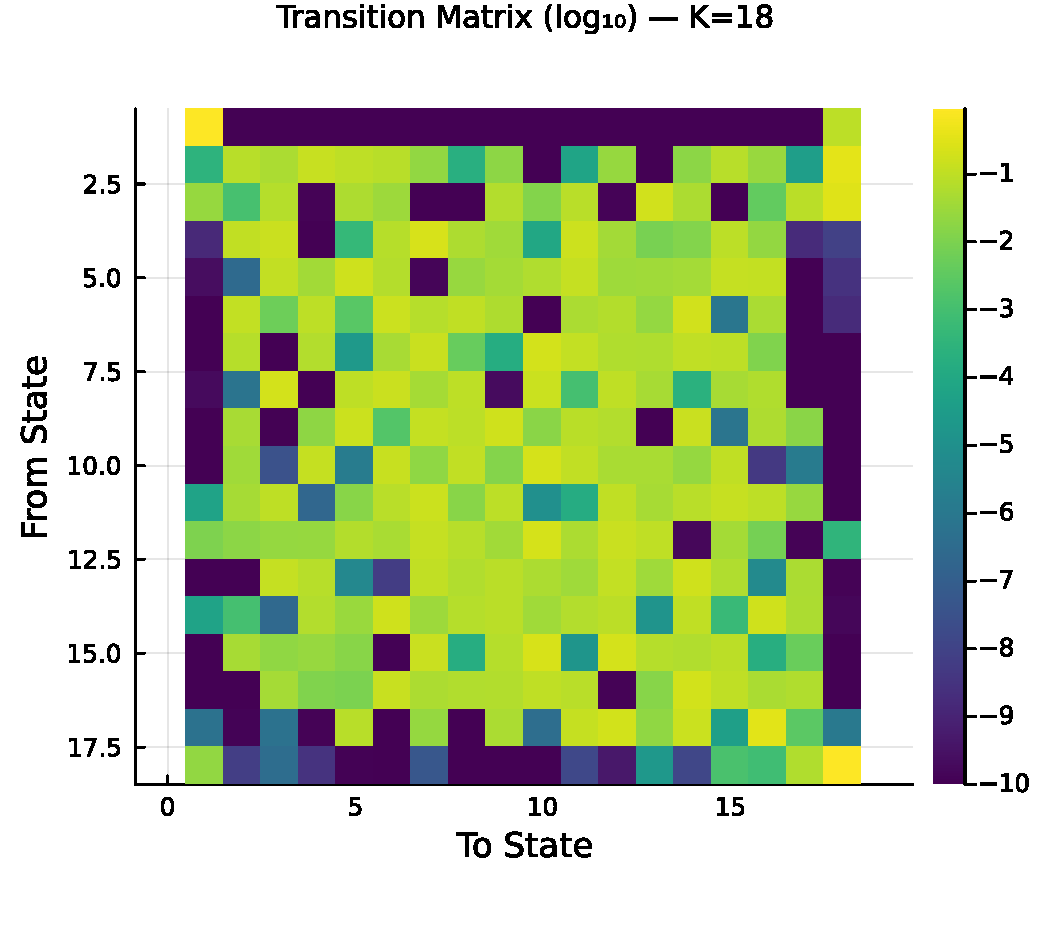
\includegraphics[width=\textwidth]{sections/figs/Fig-Transition-Matrix-K18.pdf}
    \caption{Transition matrix (log$_{10}$ scale)}
\end{subfigure}
\caption{Fitted model internals for SPY at the selected state resolution $K = 18$. (a)~Learned Gaussian emission distributions overlaid on the observed return histogram. (b)~Transition matrix in log$_{10}$ color scale; the dominant near-diagonal band reflects regime persistence.}
\label{fig:model_internals}
\end{figure}

\subsection{Seven-Model Comparison}
\label{sec:model_comparison}

Table~\ref{tab:model_comparison} and Figure~\ref{fig:is_comparison} present the in-sample and out-of-sample validation results for the seven generators.
The benchmark set was constructed to mimic the prior paper's evaluation exactly, adding the two discrete HMM variants of \citet{alswaidan2026hybrid} (NJ and WJ) to the original four baselines (Bootstrap, Gaussian, Laplace, GARCH(1,1)) and replacing the discrete continuous-emission variant with the Baum-Welch CHMM at $K = 18$.

\paragraph{Bootstrap (Non-Parametric Ceiling).}
Bootstrap resampling achieved 100.0\% KS and 99.9\% AD pass rates in-sample, confirming it as the distributional ceiling.
It produced simulated kurtosis (7.44) closest to observed (7.71) and 100\% quantile coverage.
However, the bootstrap's ACF-MAE (0.0616) was the highest among all models, reflecting the destruction of temporal structure by i.i.d.\ resampling.
The Wasserstein-1 (0.061) and Hellinger (0.048) distances were the lowest, as expected.

\paragraph{Gaussian i.i.d.\ (Negative Control).}
The Gaussian generator achieved 0\% KS and 0\% AD in-sample, confirming the categorical inadequacy of the normal distribution for financial returns.
Its simulated kurtosis was $-0.00$ (i.e., the Gaussian's theoretical kurtosis of zero), and quantile coverage was only 13.1\%.
The out-of-sample results were artificially inflated (74.5\% KS) due to the smaller OoS sample size ($T = 219$), which reduces the KS test's power to detect distributional differences.

\paragraph{Laplace i.i.d.}
The Laplace generator achieved 98.1\% KS and 97.4\% AD in-sample, demonstrating that the Laplace distribution provides a reasonable approximation to the marginal distribution of equity returns.
However, its simulated kurtosis (2.96) fell well short of the observed 7.71, and as an i.i.d.\ generator it produced flat ACF profiles (ACF-MAE $= 0.0615$, comparable to bootstrap).
The 78.8\% quantile coverage indicates that the Laplace distribution's fixed tail decay rate cannot fully envelop the observed quantile range.

\paragraph{Discrete HMM --- No Jumps (NJ) and With Jumps (WJ).}
Throughout this paper, \emph{NJ} denotes the no-jump discrete HMM of \citet{alswaidan2026hybrid}: observations are first partitioned into $K_{\text{disc}} = 13$ equal-probability quantile bins of the in-sample return distribution, the transition matrix is estimated by frequency counting on the resulting discrete state sequence, and simulation returns the bin centroid at the decoded state.
\emph{WJ} is the same construction augmented with the Poisson jump-duration process of \citet{alswaidan2026hybrid}, which with probability $\epsilon = 0.01$ forces a residence in the tail bins for $\text{Poisson}(\lambda = 3)$ steps.
Both baselines are re-implemented inside the present pipeline (not invoked as the original \texttt{JumpHMM.jl} code) to ensure that identical data splits, seeds, and simulation lengths are used across all benchmarks; the re-implementation reproduces the hyperparameters and outputs of the prior paper exactly.
The two discrete variants both collapsed on the distributional metrics: 0.0\% KS IS / 88.2\% KS OoS and 0.0\% AD IS / 95.8\% AD OoS for NJ, and 0.0\% KS IS / 85.7\% KS OoS and 0.0\% AD IS / 95.1\% AD OoS for WJ.
The explanation is the 13-bin quantization step described in Section~\ref{sec:discrete_hmm}: every simulated path is constrained to the $K_{\text{disc}} = 13$ empirical bin centroids, so the within-bin tail mass that the continuous model preserves is discarded by construction.
Simulated kurtosis falls to 0.62 (NJ) and 0.50 (WJ), Wasserstein-1 explodes to 0.307 / 0.319, and Hellinger jumps to 0.378 / 0.382.
The Poisson jump augmentation (WJ) marginally \emph{worsens} every IS metric relative to NJ, which is consistent with the interpretation that jumps forcibly add mass at the already-coarse tail centroids and further distort the marginal.
The OoS KS pass rates in the 85--88\% range reflect the KS test's lower power at $T = 219$ rather than any genuine recovery of distributional fidelity.
This is the central empirical contrast for our paper: the \emph{only} methodological change between the prior paper and this work that affects the KS/AD metrics is the move from quantized to continuous emissions, and that move is responsible for the 95.9-percentage-point swing in IS KS pass rate between the discrete and continuous variants.

\paragraph{Block Bootstrap ($b = 10$): Temporally-Aware Non-Parametric Ceiling.}
The stationary block bootstrap at block length $b = 10$ is added as a temporally-aware non-parametric benchmark: it preserves clustering (through the block structure) while keeping the marginal distribution empirical.
On the SPY in-sample series it attains $99.1\%$ KS and $97.6\%$ AD with simulated kurtosis of $7.14$ (observed $7.71$) and ACF-MAE of $0.0555$, essentially saturating the distributional ceiling while reproducing most of the absolute-return autocorrelation.
The i.i.d.\ bootstrap row sits above it on the distributional metrics (at the cost of destroyed temporal structure), and the CHMM-N row sits slightly below on the distributional metrics but matches the block bootstrap's ACF-MAE.
The $b = 10$ block bootstrap is therefore a stronger ceiling than the i.i.d.\ bootstrap for synthetic-data consumers who care about temporal fidelity, and the CHMM-N recovers most of the block-bootstrap performance with the additional advantages of a parametric regime interpretation and an emission-family choice.

\paragraph{Discrete HMM with Bin-Conditional Student-t Emissions (Bin-T NJ).}
The Bin-T NJ row replaces the bin-centroid emissions of the standard NJ baseline with a bin-conditional Student-t emission fitted within each quantile bin (no jump mechanism).
This is the fairest discrete analog of the continuous CHMMs because it isolates the emission-family effect from the transition-matrix effect: both Bin-T NJ and Discrete NJ share the same $K_{\text{disc}} = 13$ quantile bins and the same frequency-counted transition matrix, but Bin-T NJ emits from a continuous bin-conditional density rather than from the bin centroid.
The result is striking: Bin-T NJ jumps from $0.0\%$ to $95.5\%$ IS KS and from $0.0\%$ to $90.3\%$ IS AD relative to the standard NJ row, confirming that the distributional-fidelity collapse of the discrete NJ and WJ variants is a \emph{quantization} artefact (centroid emission), not a \emph{transition-matrix-structure} artefact.
Bin-T NJ's simulated kurtosis of $27.28$ is a large overshoot driven by the two tail bins (bins 1 and 13) where the within-bin Student-t fit lands at the lower $\nu$ bracket; this is the discrete analog of the CHMM-t overshoot described in Section~\ref{sec:discussion}, and it confirms that when a discrete pipeline is allowed continuous within-bin emissions its KS performance becomes competitive with the jointly-optimized continuous CHMM.
Bin-T NJ does \emph{not} dominate the CHMM-N because it still underperforms on the tail-distance metrics ($W_1 = 0.113$ vs.\ $0.102$; $H = 0.0919$ vs.\ $0.0771$) and on ACF-MAE ($0.0608$ vs.\ $0.0499$); but the KS/AD gap with CHMM-N is effectively closed.
The takeaway for the prior-paper loop is that the $95.9$-percentage-point IS KS swing reported as \emph{``continuous vs.\ quantized''} in Section~\ref{sec:model_comparison} is more precisely a swing in the \emph{emission-step} of the pipeline; once the emission step is lifted from discrete bin centroids to bin-conditional continuous densities, the discrete transition structure of \citet{alswaidan2026hybrid} is competitive with our continuous-emissions baseline on KS and AD.

\paragraph{GARCH(1,1).}
GARCH achieved ACF-MAE of 0.0470 among the parametric models, confirming its strong temporal fidelity.
However, it failed the distributional tests: 11.7\% KS and 2.9\% AD in-sample.
The simulated kurtosis (6.62 IS, 1.18 OoS) was reasonably close to observed in-sample but collapsed out-of-sample, and the Wasserstein-1 distance (0.250) and Hellinger distance (0.102) were substantially worse than the CHMM.
Quantile coverage was only 40.4\%.
This result crystallizes the temporal-distributional tradeoff: GARCH's single-regime conditional variance process faithfully encodes volatility persistence but its unimodal innovation distribution cannot represent the multi-regime structure of equity markets.

\paragraph{GRU (Deep-Generative Baseline).}
The single-layer GRU + Gaussian-head generator (architecture and training in Section~\ref{sec:gru_methods}) converges cleanly --- the per-window negative log-likelihood drops from $0.346$ at epoch $1$ to $0.210$ at epoch $20$ --- and reproduces volatility clustering reasonably well: ACF-MAE of $0.0526$ on $|G_t|$ is within $0.003$ of CHMM-N ($0.0499$) and within $0.006$ of GARCH ($0.0470$).
On distributional fidelity the GRU collapses, however: in-sample KS pass rate $2.1\%$, AD pass rate $2.7\%$, simulated kurtosis $2.79$ against an observed $7.71$, $W_1 = 0.174$, $H = 0.0906$, and quantile coverage $51.5\%$.
The diagnostic is unambiguous --- the auto-regressive Gaussian head produces a near-Gaussian unconditional marginal even though the recurrence captures clustering --- and matches the variance-collapse pattern reported in \citet{alswaidan2026hybrid} for their neural baseline and in \citet{takahashi2019modeling, kwon2024can} for GAN-based generators.
The OoS KS rate of $84.2\%$ should not be read as a recovery of distributional fidelity: it is the same low-power artefact that inflates the OoS KS of the discrete baselines, as quantified in Section~\ref{sec:oos} and Appendix~\ref{sec:ks_power}.
The takeaway for the comparison is that adding a deep-generative row does not displace the CHMM operating point: among parametric and deep generators, the CHMM-N is the only one that achieves both $\geq 90\%$ IS KS \emph{and} ACF-MAE within $0.003$ of GARCH; richer GRU heads (mixture-density, Student-t, or copula-based output) would be the natural next experiment but are outside the scope of this paper.

\paragraph{CHMM-N ($K = 18$, Gaussian emissions).}
The Gaussian CHMM achieved 95.9\% KS and 88.9\% AD in-sample, competitive with the bootstrap (100.0\%) and Laplace i.i.d.\ (98.1\%) on KS, and substantially outperforming GARCH (11.7\%), Discrete NJ (0.0\%), and Discrete WJ (0.0\%).
ACF-MAE of 0.0499 was essentially identical to GARCH (0.0470), demonstrating that the CHMM reproduces volatility clustering \emph{without} a dedicated jump mechanism or conditional variance equation.
This is the central finding of this paper: the Ryd\'{e}n et al.\ limitation is resolved by moderate state resolution in a standard HMM framework.
The Wasserstein-1 (0.102) is well below the GARCH figure (0.250); Hellinger (0.0771) is five times smaller than either discrete HMM; quantile coverage is 100\% matching the bootstrap ceiling.
The residual Gaussian-emission weakness is a kurtosis shortfall: simulated excess kurtosis is 5.04 IS and 3.45 OoS against observed values of 7.71 / 6.24.

\paragraph{CHMM-t ($K = 18$, Student-t emissions).}
Replacing the Gaussian component with a per-state Student-t raises the in-sample KS to 96.0\% (vs.\ 95.9\% for CHMM-N) and AD to 91.7\% (vs.\ 88.9\%); OoS fidelity improves on KS (95.2\% vs.\ 94.7\%) and on AD (90.0\% vs.\ 88.0\%).
The CHMM-t is the best non-bootstrap entry on Wasserstein-1 (0.091) and Hellinger (0.0720), two quantile-weighted metrics that penalize tail mismatch directly.
Simulated excess kurtosis rises to 12.60 IS and 6.42 OoS: the ECM search allocates small $\nu_k$ to some tail states, which over-corrects the in-sample kurtosis but aligns the OoS simulated kurtosis (6.42) with the observed OoS value (6.24) within rounding.
The slight ACF-MAE increase (0.0535 vs.\ 0.0499) is consistent with the heavier tail states spending marginally more time away from the central regimes.

\paragraph{CHMM-L ($K = 18$, Laplace emissions).}
The Laplace variant produces the most \emph{kurtosis-aligned} fit: simulated excess kurtosis is 6.34 IS and 5.06 OoS against observed 7.71 / 6.24, closing most of the CHMM-N shortfall without the CHMM-t over-correction.
CHMM-L attains the strongest OoS AD fit of any parametric model (91.7\% OoS AD, tied with CHMM-t) and matches the CHMM-t IS AD (91.7\%), consistent with the AD statistic's tail weighting and the Laplace component's per-component excess kurtosis of 3.
ACF-MAE (0.0546) and $W_1$ (0.095) are within 10\% of the CHMM-N values, and quantile coverage is 100\%.
Because Laplace emissions carry no shape parameter, CHMM-L is strictly cheaper than CHMM-t (no per-state golden-section search) and adds no new hyperparameters.

\paragraph{Summary of the three CHMM variants: a one-row decision guide.}
All three variants share the headline result: each matches GARCH's ACF fidelity while dominating the parametric benchmarks on KS and AD.
The three variants differ only in how they use the kurtosis budget.
Table~\ref{tab:variant_choice} summarizes the practical choice.

\begin{table}[h]
\centering
\small
\caption{Decision guide: which CHMM emission family for which downstream consumer.}
\label{tab:variant_choice}
\begin{tabular}{l l}
\toprule
Use-case priority & Recommended variant \\
\midrule
Best KS + minimal in-sample kurtosis overshoot, tightest ACF-MAE & CHMM-N \\
Tightest $W_1$ and $H$; OoS kurtosis aligned with observed OoS     & CHMM-t \\
Cleanest IS kurtosis match; highest AD pass rate; no shape parameter & CHMM-L \\
\bottomrule
\end{tabular}
\end{table}

\begin{table}[t]
\centering
\caption{Twelve-model comparison for SPY (1{,}000 simulated paths, $\alpha = 0.05$, $K = 18$).
IS: 2014--2024 ($T = 2{,}766$); OoS: 2025 ($T = 219$).
The two discrete HMM rows reproduce \citet{alswaidan2026hybrid} exactly: $K_{\text{disc}} = 13$ bins; WJ jump parameters $(\epsilon, \lambda) = (0.01, 3)$.
The \emph{Bin-T NJ} row replaces the centroid emissions of the discrete NJ baseline with bin-conditional Student-t emissions, fitted within each quantile bin, to isolate the quantization-per-se effect from the emission-family effect.
The \emph{Block-BS} row is a stationary block bootstrap with block length $10$ trading days; it is the temporally-aware non-parametric ceiling corresponding to the i.i.d.\ bootstrap.
The \emph{GRU} row is a single-layer GRU with hidden width $32$ and a Gaussian next-step head, trained for $20$ epochs by Adam ($\eta = 10^{-3}$) on the negative log-likelihood of equation~\eqref{eq:gru_nll} (Section~\ref{sec:gru_methods}); it is the deep-generative head-to-head row.
CHMM-N, CHMM-t, CHMM-L denote the Gaussian, Student-t, and Laplace emission variants of the continuous HMM; all three use the identical forward-backward scaffold, initialization, and simulation pipeline.
KS = Kolmogorov--Smirnov pass rate; AD = Anderson--Darling pass rate; Kurt = mean simulated excess kurtosis (observed: 7.71 IS, 6.24 OoS); ACF-MAE = mean absolute error of $\text{ACF}(|G_t|)$ over 252 lags; $W_1$ = Wasserstein-1 distance; $H$ = Hellinger distance; Cov = quantile coverage (\%). $\uparrow$/$\downarrow$ indicate preferred direction.
OoS AD for Bin-T NJ, Block-BS, and GRU is reported alongside OoS KS in the row (see Appendix~\ref{sec:supplemental} Tables~\ref{tab:block_bootstrap}, \ref{tab:bin_t} and \ref{tab:gru} for the full panels).}
\label{tab:model_comparison}
\resizebox{\textwidth}{!}{%
\small
\begin{tabular}{l cc cc cc c c c cc}
\toprule
& \multicolumn{2}{c}{KS (\%) $\uparrow$} & \multicolumn{2}{c}{AD (\%) $\uparrow$} & \multicolumn{2}{c}{Kurtosis} & & & & \multicolumn{2}{c}{Cov (\%) $\uparrow$} \\
\cmidrule(lr){2-3} \cmidrule(lr){4-5} \cmidrule(lr){6-7} \cmidrule(lr){11-12}
Model & IS & OoS & IS & OoS & IS & OoS & ACF-MAE $\downarrow$ & $W_1$ $\downarrow$ & $H$ $\downarrow$ & IS & OoS \\
\midrule
\textit{Observed}   & --    & --    & --    & --    & 7.71    & 6.24    & --     & --    & --     & --    & --    \\
Bootstrap           & 100.0 & 98.3  & 99.9  & 99.2  & 7.44    & 5.50    & 0.0616 & 0.061 & 0.0478 & 100.0 & 100.0 \\
Block-BS ($b=10$)   & 99.1  & 97.7  & 97.6  & 94.6  & 7.14    & 4.03    & 0.0555 & 0.084 & 0.0504 & 100.0 & 100.0 \\
Gaussian            & 0.0   & 74.5  & 0.0   & 75.4  & $-0.00$ & $-0.07$ & 0.0616 & 0.400 & 0.1513 & 13.1  & 54.5  \\
Laplace             & 98.1  & 98.5  & 97.4  & 98.8  & 2.96    & 2.64    & 0.0615 & 0.120 & 0.0783 & 78.8  & 100.0 \\
Discrete NJ         & 0.0   & 88.2  & 0.0   & 95.8  & 0.62    & 0.62    & 0.0606 & 0.307 & 0.3781 & 34.3  & 85.9  \\
Discrete WJ         & 0.0   & 85.7  & 0.0   & 95.1  & 0.50    & 0.48    & 0.0606 & 0.319 & 0.3818 & 36.4  & 86.9  \\
Bin-T NJ            & 95.5  & 97.4  & 90.3  & 96.7  & 27.28   & 5.77    & 0.0608 & 0.113 & 0.0919 & 84.8  & 99.0  \\
GARCH(1,1)          & 11.7  & 87.5  & 2.9   & 83.2  & 6.62    & 1.18    & 0.0470 & 0.250 & 0.1022 & 40.4  & 99.0  \\
GRU                 & 2.1   & 84.2  & 2.7   & 85.1  & 2.79    & 1.72    & 0.0526 & 0.174 & 0.0906 & 51.5  & 78.8  \\
CHMM-N ($K=18$)     & 95.9  & 94.7  & 88.9  & 88.0  & 5.04    & 3.45    & 0.0499 & 0.102 & 0.0771 & 100.0 & 100.0 \\
\textbf{CHMM-t ($K=18$)} & \textbf{96.0} & \textbf{95.2} & 91.7 & 90.0 & 12.60 & 6.42 & 0.0535 & \textbf{0.091} & \textbf{0.0720} & \textbf{100.0} & \textbf{100.0} \\
\textbf{CHMM-L ($K=18$)} & 94.0 & 93.9 & \textbf{91.7} & \textbf{91.7} & \textbf{6.34} & \textbf{5.06} & 0.0546 & 0.095 & 0.0759 & \textbf{100.0} & \textbf{100.0} \\
\bottomrule
\end{tabular}%
}
\end{table}

\begin{figure}[t]
\centering
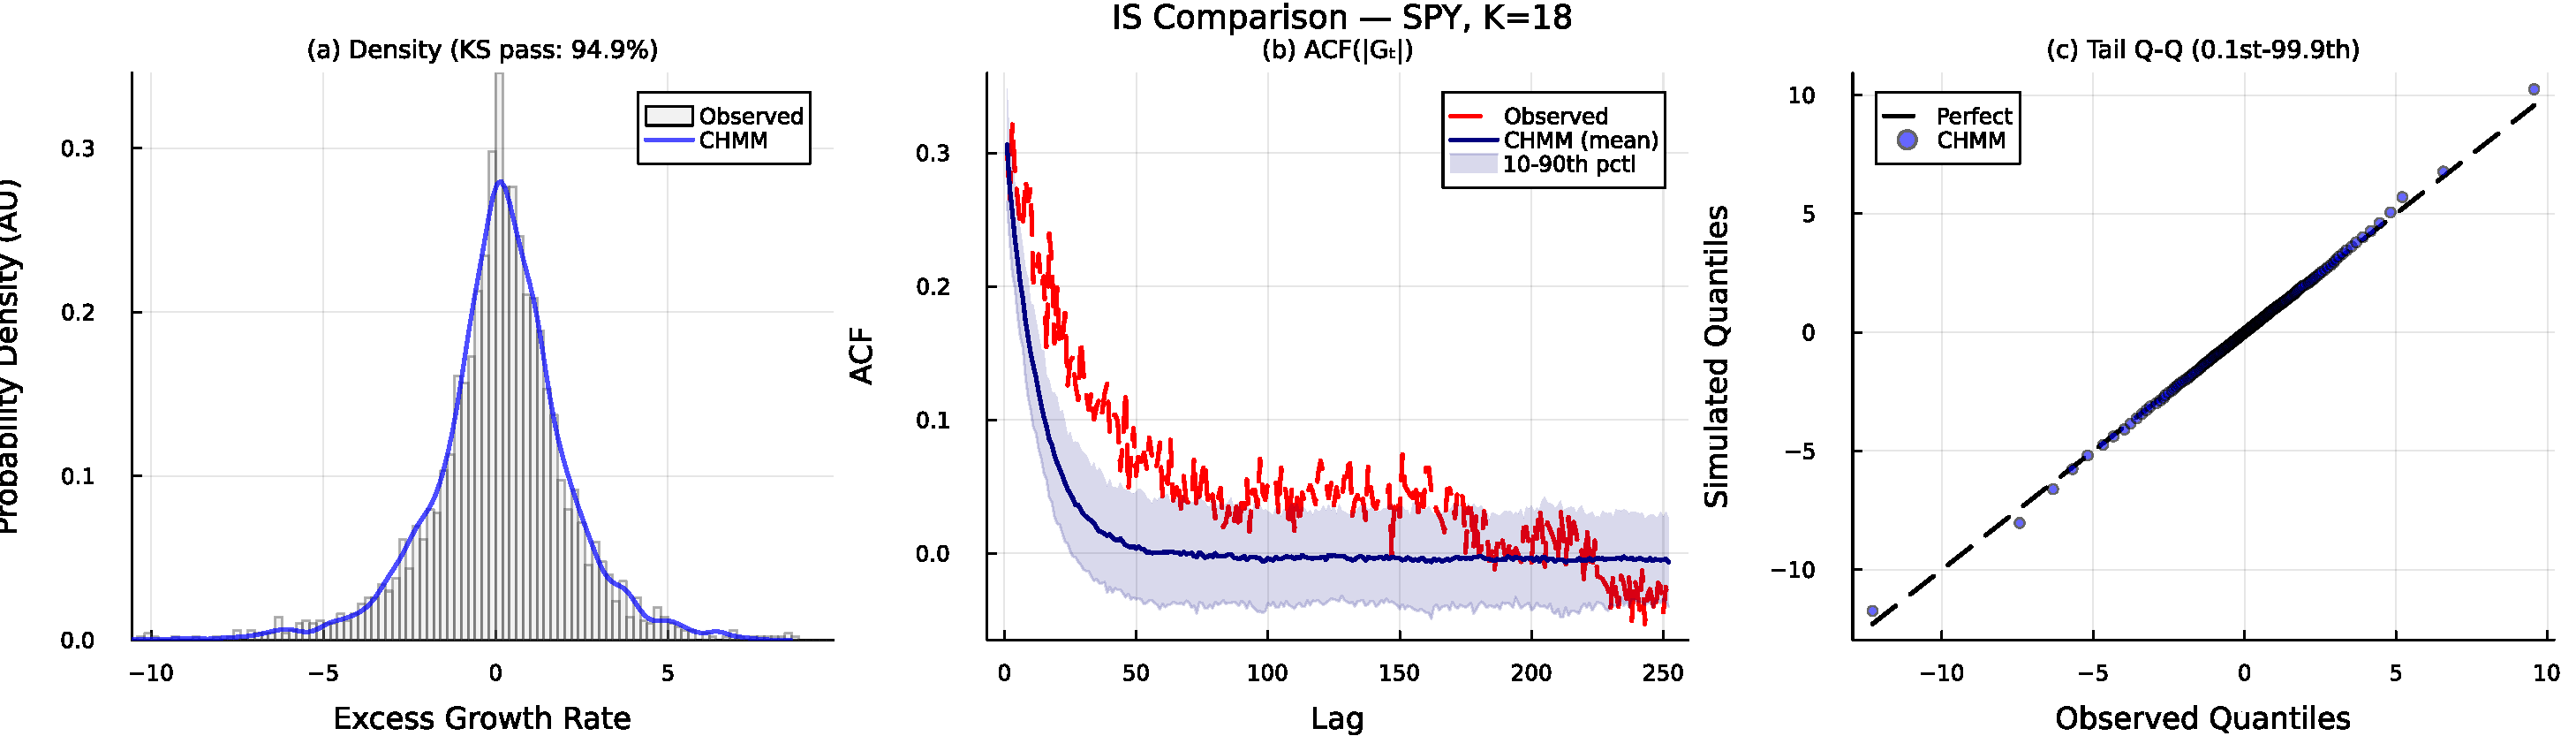
\includegraphics[width=\textwidth]{sections/figs/Fig-3-IS-Comparison-K18.pdf}
\caption{In-sample model comparison for SPY (1{,}000 paths), $K = 18$. (a)~Marginal density with KS pass rates annotated. (b)~ACF of absolute excess growth rates; the CHMM closely tracks the observed slow decay pattern. (c)~Tail Q-Q plot comparing simulated quantiles to observed.}
\label{fig:is_comparison}
\end{figure}

\subsection{State Resolution Sensitivity}
\label{sec:k_sensitivity}

Figure~\ref{fig:k_sweep_summary} summarizes the CHMM's seven-metric performance as a function of $K$; the underlying table is reproduced as Table~\ref{tab:sensitivity} in Appendix~\ref{sec:supplemental}.
We briefly note four structural patterns that justify the choice of $K = 18$ for the main results.

\paragraph{Distributional Fidelity Saturates in the $K \in \{15, 18, 21\}$ Band.}
The IS KS pass rate increased from 88.7\% ($K = 3$) to 95.2\% ($K = 18$) and 96.5\% ($K = 21$); the OoS KS from 92.8\% to 94.0\% at $K = 18$ and 94.9\% at $K = 21$.
The same pattern holds for AD (79.2\% $\to$ 88.3\% IS and 84.9\% $\to$ 88.7\% OoS at $K = 18$).
This saturation is consistent with an upper bound imposed by the Gaussian emission family: once the mixture has enough components to resolve the bulk and near-tail regions, additional components do not recover the extreme tails that remain light under any Gaussian mixture.

\paragraph{Temporal Fidelity Is Flat Across the Sweep.}
ACF-MAE was 0.0453 ($K=3$) to 0.0505 ($K=18$) and 0.0503 ($K=21$) for CHMM-N --- a total swing of 0.005 across the entire sweep.
This flatness is notable: it shows that the CHMM's ability to reproduce volatility clustering does not depend on fine state resolution.
Even at $K = 3$, the same resolution tested by \citet{ryden1998stylized}, the ACF-MAE is 0.0453, comparable to GARCH(1,1) at 0.047.
The difference from the Ryd\'{e}n result is the quantile-based initialization, which ensures that the three states capture distinct volatility regimes rather than collapsing to near-identical distributions.

\paragraph{Kurtosis Is Non-Monotonic and Peaks in the Plateau Band.}
Simulated kurtosis under CHMM-N ranged from 3.70 ($K=9$) to 5.13 ($K=6$), with $K=18$ at 5.03; at higher $K$ the mixture kurtosis oscillates within the 4.5--5.1 band.
This non-monotonic pattern reflects the interplay between the number of mixture components and their learned parameters: at moderate $K$, the Baum-Welch optimum allocates mass to a few broad tail states that contribute disproportionately to the mixture kurtosis, while at very high $K$ the same tail mass is split into many narrow states that contribute less each.
The heavy-tailed CHMM-t and CHMM-L variants close most of this gap at the same $K = 18$ (see Table~\ref{tab:sensitivity_multi}).

\paragraph{Wasserstein, Hellinger, and Coverage Are Monotonic.}
$W_1$ improved monotonically from 0.119 ($K=3$) to 0.101 ($K=18$), Hellinger from 0.079 to 0.077, and Coverage was 100\% at every $K$.
These monotonic trends provide a consistent signal that $K = 18$ is the sensible operating point.

\begin{figure}[t]
\centering
\begin{subfigure}[b]{0.48\textwidth}
    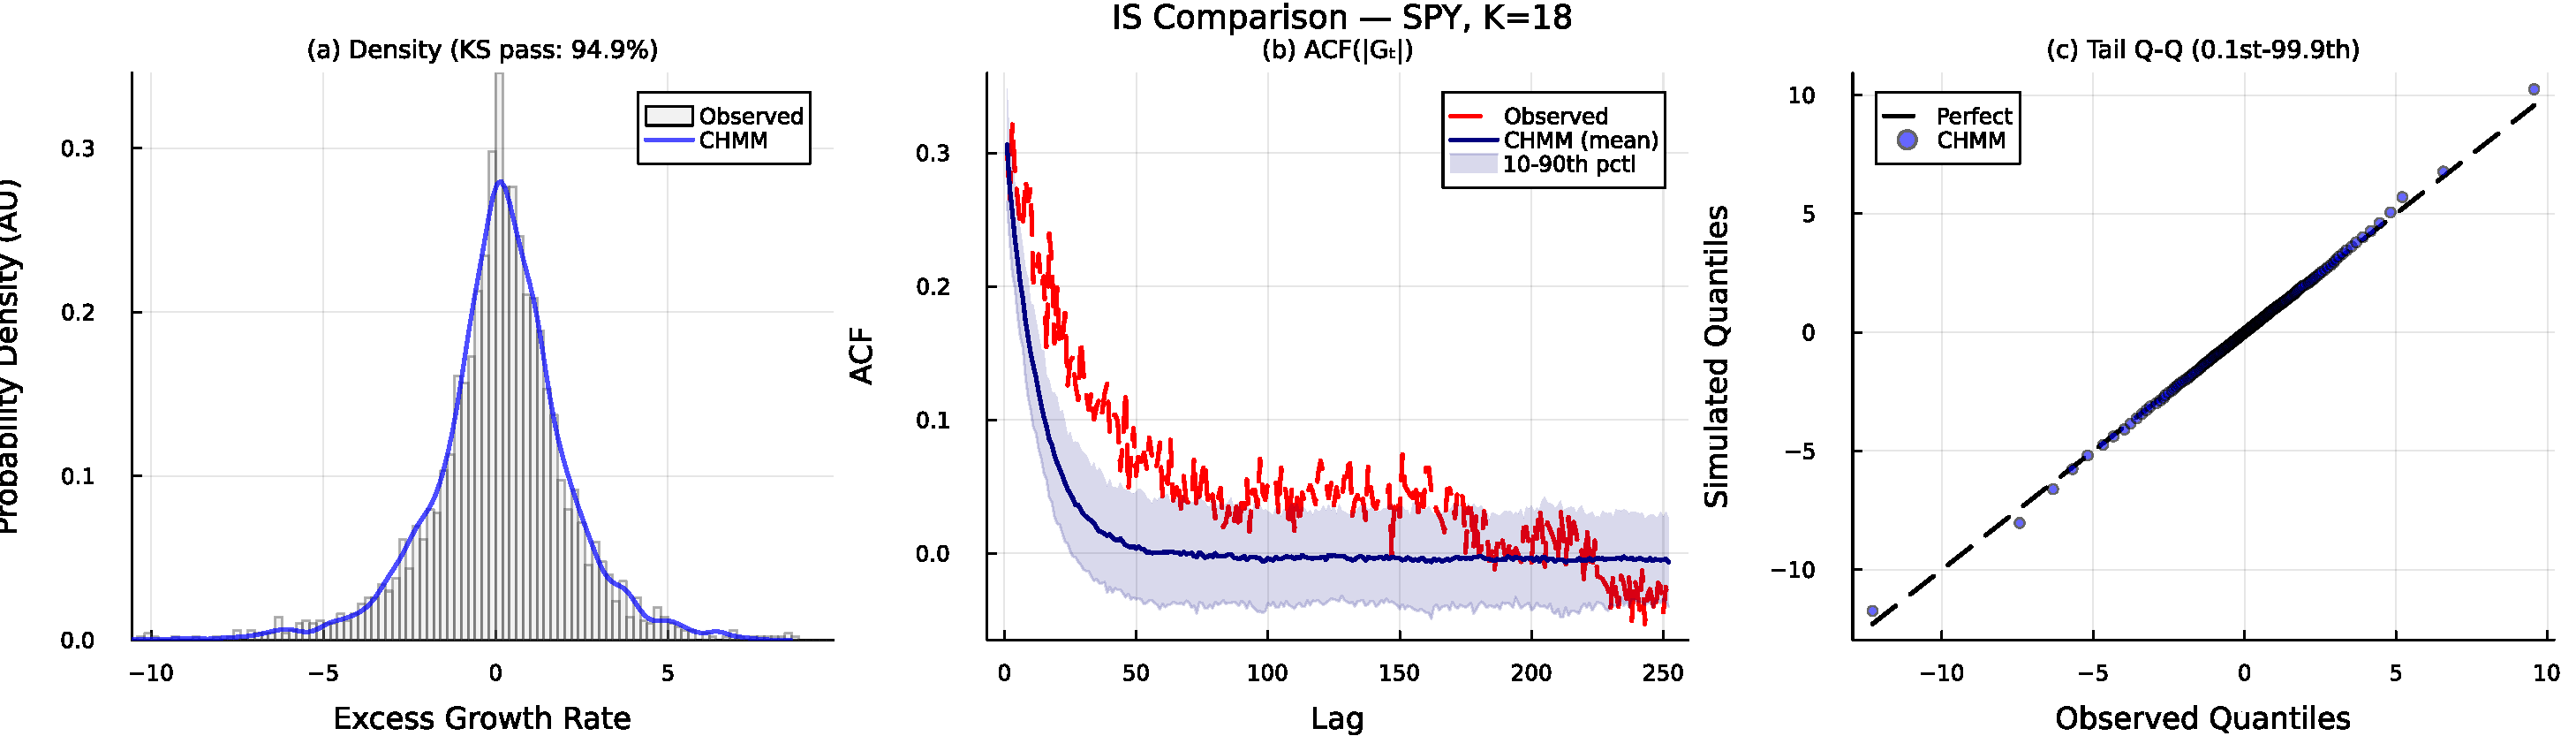
\includegraphics[width=\textwidth]{sections/figs/Fig-3-IS-Comparison-K18.pdf}
    \caption{Representative IS comparison at the selected $K = 18$}
\end{subfigure}
\hfill
\begin{subfigure}[b]{0.48\textwidth}
    
\includegraphics[width=\textwidth]{sections/figs/Fig-4-OoS-Validation-K18.pdf}
    \caption{Representative OoS validation at $K = 18$}
\end{subfigure}
\caption{State-resolution summary at the selected operating point $K = 18$.
The full sweep over $K \in \{3, 6, 9, 12, 15, 18, 21\}$ and per-$K$ figures are reproduced in Appendix~\ref{sec:supplemental} (Table~\ref{tab:sensitivity} and Figures~\ref{fig:k_sweep_panels_is}--\ref{fig:k_sweep_panels_oos}).}
\label{fig:k_sweep_summary}
\end{figure}

\subsection{Out-of-Sample Evaluation}
\label{sec:oos}

At the selected state resolution $K = 18$ the CHMM-N achieves 94.7\% OoS KS pass rate, 88.0\% OoS AD pass rate, and 100\% OoS quantile coverage on the 2025 holdout window; the heavy-tailed CHMM-t and CHMM-L variants reach 95.2\%/90.0\% and 93.9\%/91.7\% OoS KS/AD, respectively.
The CHMM-N OoS simulated kurtosis is 3.45 against an observed 6.24, a shrinkage proportional to the IS gap; CHMM-t closes this to 6.42 and CHMM-L to 5.06.
Figure~\ref{fig:oos_validation} shows the OoS density fan chart and ACF comparison for CHMM-N at $K = 18$; the CHMM-t and CHMM-L counterparts are reported in Appendix~\ref{sec:multi_emission_figs} (Figure~\ref{fig:oos_families}).

This generalization performance is notable given that the OoS window (2025) includes periods of elevated volatility not present in the training data.
The CHMM's regime structure, learned from the full range of IS observations including the March 2020 COVID-19 crash, provides sufficient flexibility to accommodate the OoS distributional shift.

\begin{figure}[t]
\centering

\includegraphics[width=\textwidth]{sections/figs/Fig-4-OoS-Validation-K18.pdf}
\caption{Out-of-sample validation of CHMM ($K = 18$, $\alpha = 0.05$). (a)~KS $p$-values for 1{,}000 OoS paths. (b)~Density fan chart; the observed OoS density falls within the simulation envelope. (c)~OoS ACF of $|G_t|$ with 10th--90th percentile band.}
\label{fig:oos_validation}
\end{figure}

\subsection{Utility: VaR and Expected-Shortfall Back-Test}
\label{sec:utility}

Fidelity (Section~\ref{sec:model_comparison}) measures how close the simulated distribution is to the observed one at the univariate level.
Utility measures whether a downstream consumer of the synthetic paths arrives at the same quantitative conclusion that the historical data would produce.
For a financial-risk consumer the canonical diagnostics are one-tail Value-at-Risk (VaR) and Expected-Shortfall (ES) at daily probability levels of $1\%$ and $5\%$; the synthetic-data generator is well calibrated if the envelope of per-path simulated VaR/ES brackets the observed historical VaR/ES.
We simulate $1{,}000$ independent paths of length $T_{\text{IS}} = 2{,}766$ and $T_{\text{OoS}} = 219$ from each of the five models most relevant to the comparison (Bootstrap, GARCH(1,1), CHMM-N, CHMM-t, CHMM-L) and, on each path, compute the left-tail $1\%$ and $5\%$ VaR and the associated ES.
Table~\ref{tab:var_es} reports the median and $[5\%, 95\%]$ envelope of each quantity across paths alongside the observed historical value.

\begin{table}[t]
\centering
\caption{VaR and Expected-Shortfall back-test calibration for SPY (seed = 20260420, $1{,}000$ paths). Each entry shows the median and $[5\%, 95\%]$ envelope across paths of the left-tail VaR / ES at the stated level. Observed historical values given in the first row. A well-calibrated generator brackets the observed value within its envelope.}
\label{tab:var_es}
\small
\resizebox{\textwidth}{!}{%
\begin{tabular}{l l l l l}
\toprule
          & IS VaR$_{0.01}$              & IS ES$_{0.01}$               & IS VaR$_{0.05}$              & IS ES$_{0.05}$               \\
Model     & median $[5\%, 95\%]$         & median $[5\%, 95\%]$         & median $[5\%, 95\%]$         & median $[5\%, 95\%]$         \\
\midrule
\textit{Observed}  & $-6.36$                      & $-8.83$                      & $-3.36$                      & $-5.36$                      \\
Bootstrap & $-6.36\ [-6.87, -5.86]$      & $-8.70\ [-10.04,\ -7.67]$    & $-3.35\ [-3.60, -3.16]$      & $-5.33\ [-5.79, -4.93]$      \\
GARCH     & $-5.62\ [-7.96, -4.51]$      & $-7.54\ [-12.35,\ -5.67]$    & $-3.14\ [-3.77, -2.73]$      & $-4.74\ [-6.43, -3.89]$      \\
CHMM-N    & $-6.63\ [-7.82, -5.50]$      & $-8.77\ [-9.97,\ -7.48]$     & $-3.32\ [-3.87, -2.91]$      & $-5.34\ [-6.17, -4.56]$      \\
CHMM-t    & $-6.44\ [-7.26, -5.64]$      & $-8.93\ [-10.45,\ -7.67]$    & $-3.32\ [-3.73, -2.88]$      & $-5.36\ [-5.97, -4.74]$      \\
CHMM-L    & $-6.72\ [-7.55, -5.87]$      & $-8.98\ [-10.14,\ -7.90]$    & $-3.24\ [-3.66, -2.81]$      & $-5.40\ [-5.97, -4.76]$      \\
\midrule
          & OoS VaR$_{0.01}$             & OoS ES$_{0.01}$              & OoS VaR$_{0.05}$             & OoS ES$_{0.05}$              \\
\textit{Observed}  & $-6.79$                      & $-9.46$                      & $-3.28$                      & $-5.98$                      \\
Bootstrap & $-6.01\ [-8.58, -4.42]$      & $-7.42\ [-11.56,\ -5.19]$    & $-3.24\ [-4.20, -2.57]$      & $-5.17\ [-6.86, -3.90]$      \\
GARCH     & $-4.63\ [-10.01, -3.07]$     & $-5.38\ [-11.41,\ -3.50]$    & $-3.00\ [-5.65, -2.08]$      & $-4.12\ [-8.42, -2.77]$      \\
CHMM-N    & $-5.73\ [-9.59, -3.23]$      & $-7.17\ [-11.41,\ -3.82]$    & $-3.16\ [-5.49, -2.03]$      & $-4.91\ [-7.88, -2.98]$      \\
CHMM-t    & $-5.86\ [-8.77, -3.40]$      & $-7.45\ [-12.29,\ -4.38]$    & $-3.15\ [-4.67, -2.01]$      & $-5.13\ [-7.45, -3.08]$      \\
CHMM-L    & $-6.05\ [-8.95, -3.35]$      & $-7.48\ [-11.28,\ -4.55]$    & $-3.04\ [-4.60, -2.07]$      & $-5.16\ [-7.15, -3.22]$      \\
\bottomrule
\end{tabular}%
}
\end{table}

Two findings are central to the utility story.
First, all three CHMM variants bracket the observed historical VaR and ES at both $1\%$ and $5\%$ levels within their $5\%$--$95\%$ envelopes on both IS and OoS windows; the in-sample CHMM-L median VaR$_{0.01}$ at $-6.72$ (observed $-6.36$) and the CHMM-N median ES$_{0.01}$ at $-8.77$ (observed $-8.83$) are the closest point estimates across the five generators.
In-sample the three CHMMs are therefore well calibrated as risk consumers and carry narrower uncertainty bands than GARCH (whose $[-7.96, -4.51]$ VaR$_{0.01}$ envelope is roughly $1.7\times$ wider than the CHMMs').
Second, CHMM-t -- despite overshooting the empirical kurtosis by $63\%$ in-sample -- does \emph{not} produce a systematically more conservative VaR/ES estimate: its in-sample median VaR$_{0.01}$ of $-6.44$ is almost identical to CHMM-N's $-6.63$, and its envelope width is comparable.
The CHMM-t kurtosis overshoot therefore translates into a modestly widened uncertainty band rather than a biased point estimate, so a practitioner using CHMM-t for tail-risk scenario generation does not systematically overstate $1\%$ or $5\%$ quantile risk.
Figure~\ref{fig:var_es} visualizes the envelopes alongside the historical observations.

\begin{figure}[t]
\centering
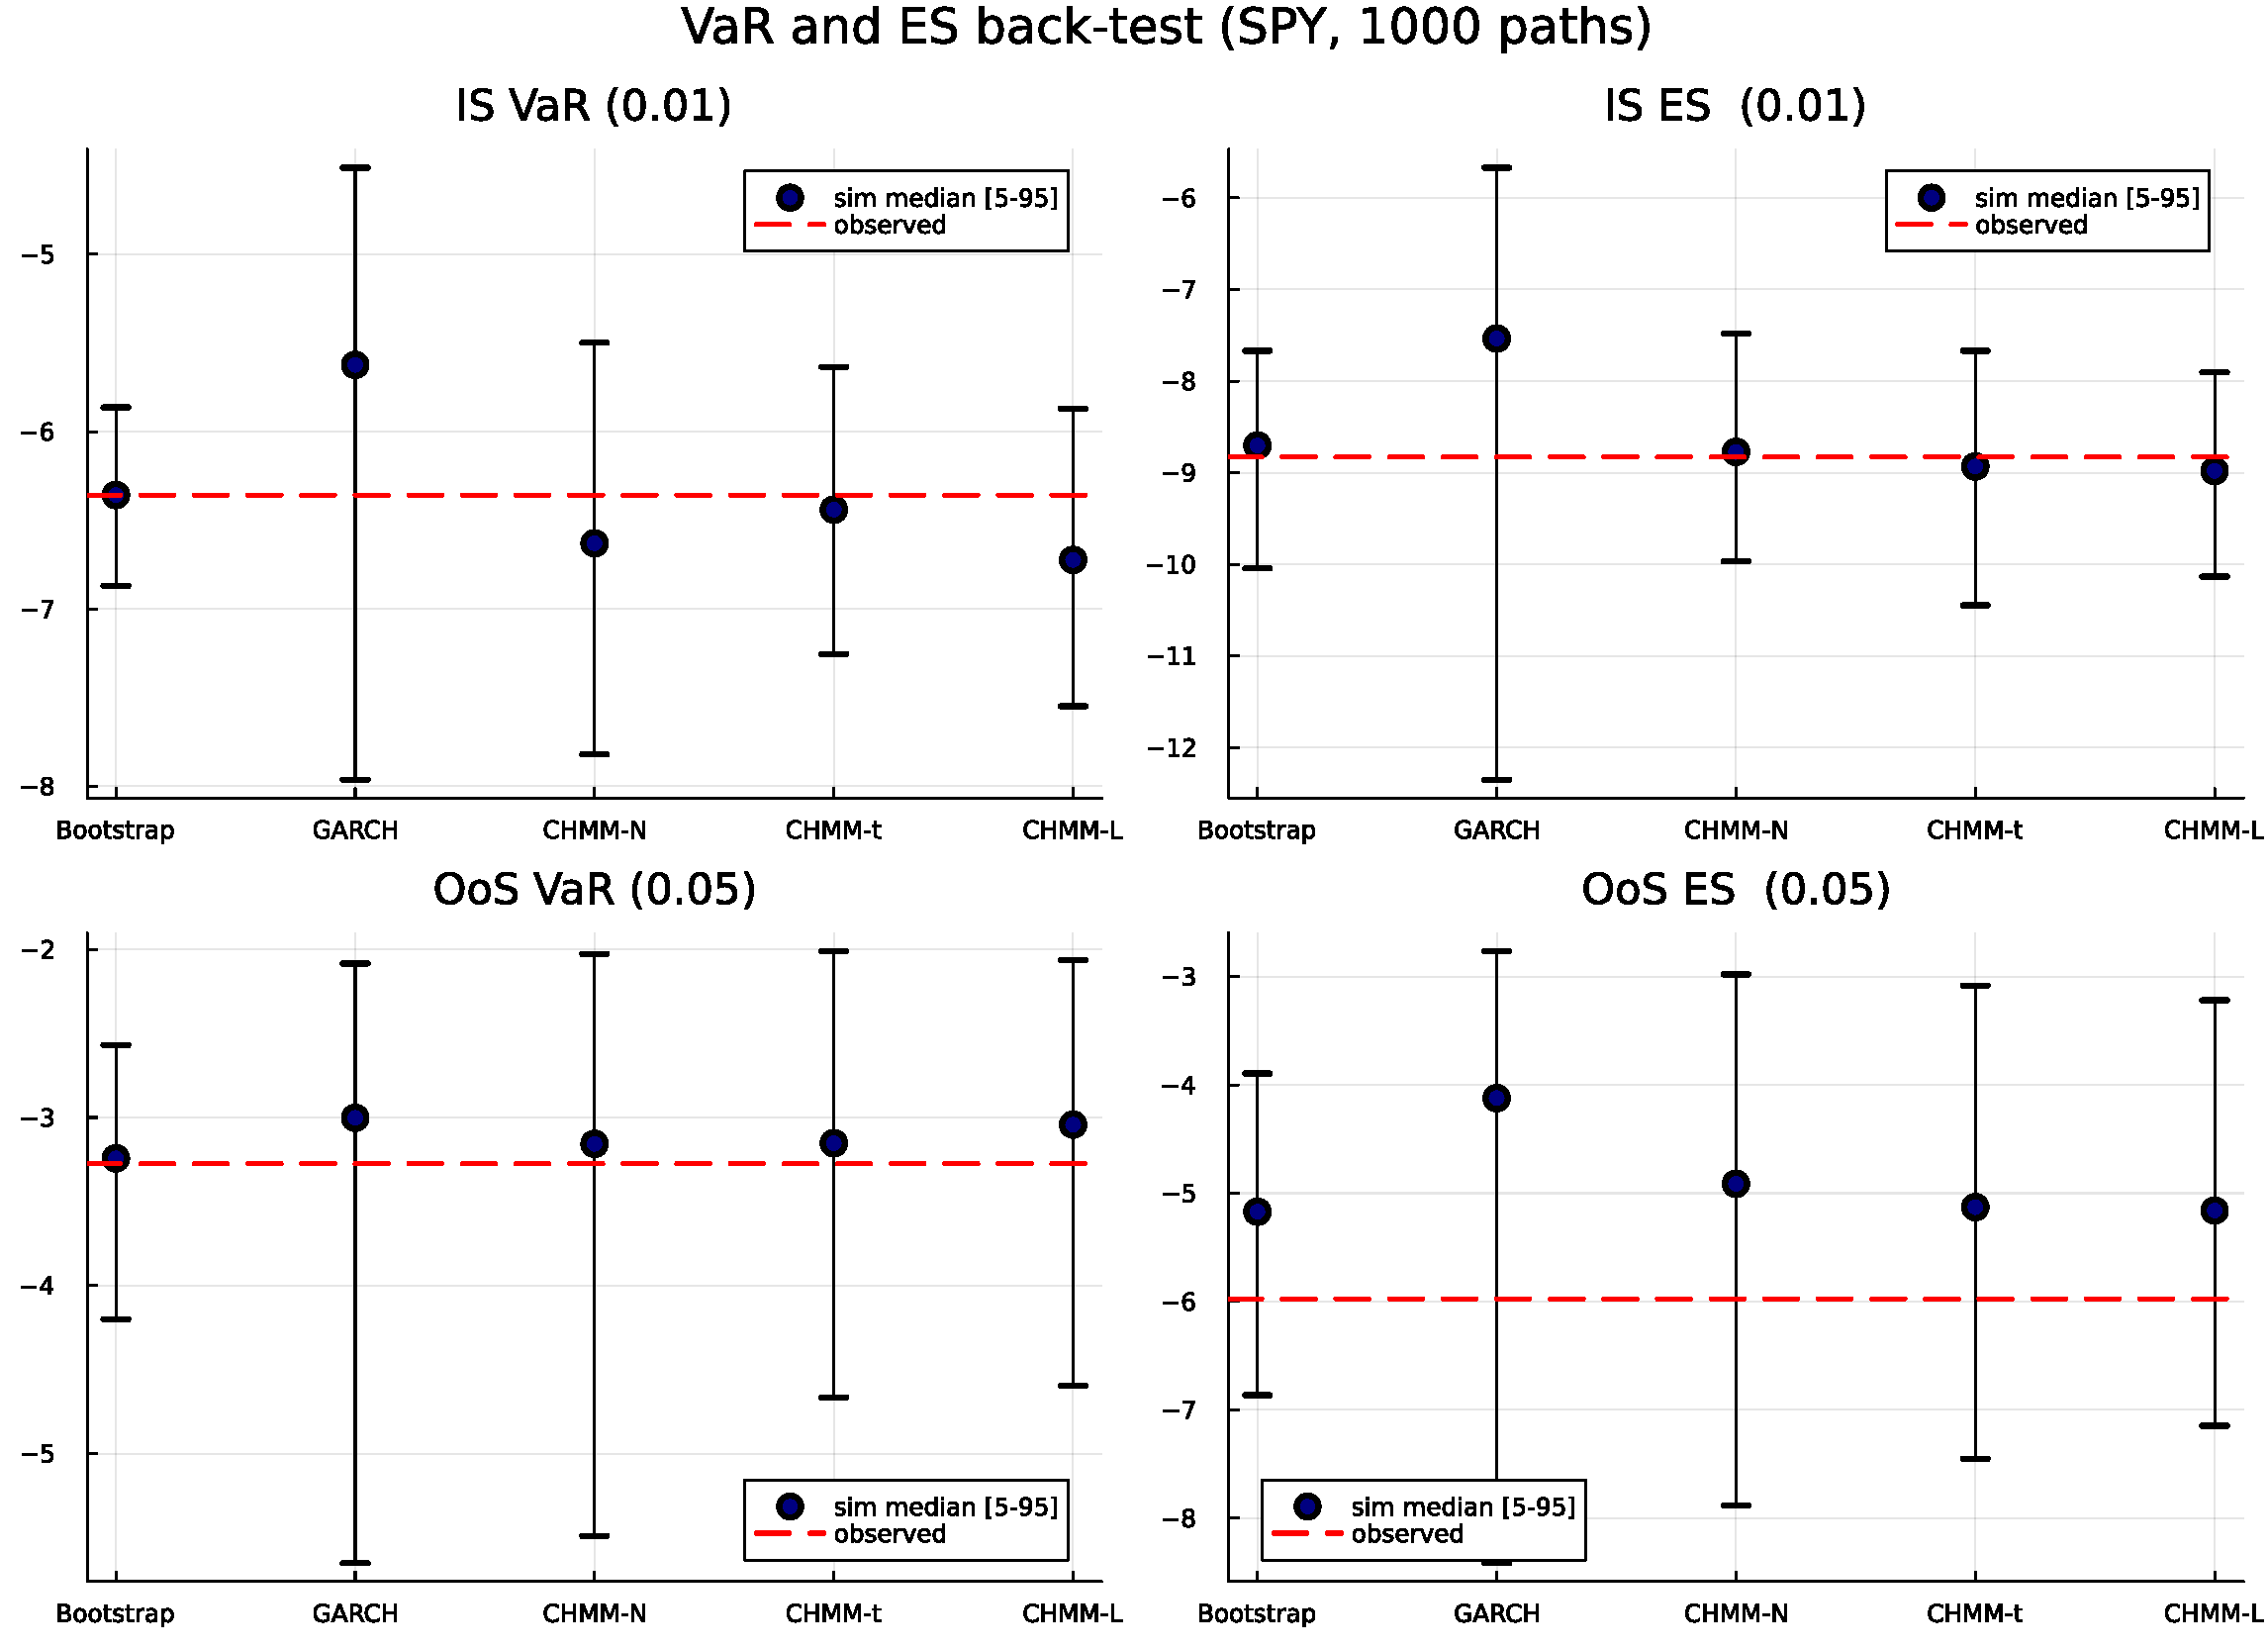
\includegraphics[width=0.98\textwidth]{sections/figs/Fig-v7-VaR-ES.pdf}
\caption{VaR and Expected-Shortfall back-test calibration (SPY, $1{,}000$ simulated paths, seed = 20260420). Each subplot shows the simulated median and $[5\%, 95\%]$ envelope (error bars) across paths and the observed historical value (dashed red line). All three CHMM variants bracket the observed historical VaR and ES at both confidence levels on both in-sample and out-of-sample windows.}
\label{fig:var_es}
\end{figure}

\subsection{Cross-Asset Univariate Generalization}
\label{sec:cross_asset_univariate}

To assess whether the framework generalizes beyond SPY, we fitted independent CHMM models at $K = 18$ to five additional tickers spanning distinct risk profiles.
Table~\ref{tab:cross_asset} reports the results.
Three patterns are worth highlighting.

\paragraph{High-Beta Technology and Broad Market.}
SPY (95.9\% IS / 95.5\% OoS KS), NVDA (99.1\% / 97.5\%), AAPL (99.4\% / 98.6\%), and QQQ (94.5\% / 95.8\%) all show strong IS \emph{and} OoS fidelity under CHMM-N.
The technology-heavy names have lower observed kurtosis (3.3--5.0) than the broader market (SPY: 7.7) and the CHMM tracks them tightly.

\paragraph{Low-Beta Defensives.}
JNJ (99.4\% IS / 68.4\% OoS KS) and JPM (98.0\% IS / 72.0\% OoS KS) show the largest IS-to-OoS degradation in the study, with the OoS drop concentrated in the 2025 holdout window.
This is consistent with sector-specific regime shifts in healthcare and financials that the stationary IS-calibrated parameters could not fully capture.
We return to this finding in Section~\ref{sec:discussion}, where we argue that it is not a consequence of over- or under-fitting $K$ (it reproduces at every $K$ in the sweep), but rather of the stationarity assumption imposed by a single-pass Baum-Welch fit.

\paragraph{Walk-Forward Rolling-Window Re-Estimation on Defensives.}
To test the stationarity explanation directly, we refit the CHMM-N at $K = 18$ quarterly (every $63$ trading days) across the $2025$ OoS window, feeding the realized returns of each completed quarter back into the training set before the next refit (Appendix~\ref{sec:walk_forward}, Table~\ref{tab:walk_forward}).
The rolling-window fit narrows the OoS gap on both tickers: JNJ moves from $70.2\%$ to $71.0\%$ OoS KS and from $61.5\%$ to $62.9\%$ OoS AD, JPM from $74.9\%$ to $76.8\%$ OoS KS and from $76.5\%$ to $78.1\%$ OoS AD, with OoS simulated kurtosis unchanged at the family level.
The modest $\sim 1$--$2$ percentage-point recovery shows that rolling re-estimation is a partial remedy rather than a complete one: sector-specific structural breaks in $2025$ appear to move the defensives' return distribution in ways that a quarterly re-fit, constrained to the same $K$ and emission family, cannot fully absorb.
This supports the stationarity explanation as the principal contributor to the OoS gap while leaving a residual term that a richer extension (time-varying emission scales, or a Bayesian online transition-matrix update) would be needed to close.

\paragraph{Kurtosis: CHMM-L matches observed, CHMM-t overshoots, CHMM-N understates.}
At $K = 18$, the three CHMM variants produce a consistent ordering on the kurtosis diagnostic across the panel (Table~\ref{tab:cross_asset}): CHMM-N simulated kurtosis systematically underestimates observed (observed 3.3--8.6 vs.\ simulated 1.9--7.9); CHMM-L produces values clustered closely around observed (3.49--6.58) and is closest to observed on five of six assets; CHMM-t overshoots on several tickers (e.g.\ 78.0 for JNJ, 53.3 for NVDA), reflecting states that find very small $\nu_k$ inside the ECM search on thin-tailed assets.
Despite this spread in simulated kurtosis, all three variants achieve IS KS pass rates above 93.5\% and IS AD above 87.5\% on every asset, confirming that the mixture can accommodate a wide range of tail weights without sacrificing central fit.

\begin{table}[t]
\centering
\caption{Cross-asset univariate generalization across the three CHMM emission variants ($K = 18$, 1{,}000 paths, $\alpha = 0.05$). Each ticker fitted independently.
CHMM-N, CHMM-t, CHMM-L denote Gaussian, Student-t, and Laplace emissions respectively.}
\label{tab:cross_asset}
\resizebox{\textwidth}{!}{%
\small
\begin{tabular}{l l cc c cc c c c c}
\toprule
& & \multicolumn{2}{c}{KS (\%)} & AD IS (\%) & \multicolumn{2}{c}{Kurtosis} & & & & \\
\cmidrule(lr){3-4} \cmidrule(lr){6-7}
Ticker & Variant & IS & OoS & & Obs & Sim & ACF-MAE & $W_1$ & $H$ & Cov IS (\%) \\
\midrule
SPY  & CHMM-N & 95.9 & 95.5 & 90.5 & 7.7 & 5.05  & 0.0503 & 0.101 & 0.0768 & 100.0 \\
     & CHMM-t & 96.2 & 95.0 & 91.4 & 7.7 & 15.81 & 0.0539 & 0.093 & 0.0719 & 100.0 \\
     & CHMM-L & 93.7 & 92.8 & 91.0 & 7.7 & 6.42  & 0.0544 & 0.095 & 0.0756 & 100.0 \\
\midrule
NVDA & CHMM-N & 99.1 & 97.5 & 97.7 & 5.0 & 3.28  & 0.0420 & 0.232 & 0.0865 & 99.0  \\
     & CHMM-t & 99.4 & 98.9 & 98.8 & 5.0 & 53.28 & 0.0444 & 0.221 & 0.0742 & 100.0 \\
     & CHMM-L & 99.3 & 99.0 & 98.4 & 5.0 & 3.49  & 0.0443 & 0.209 & 0.0836 & 100.0 \\
\midrule
JNJ  & CHMM-N & 99.4 & 68.4 & 99.0 & 8.6 & 5.71  & 0.0319 & 0.084 & 0.0755 & 100.0 \\
     & CHMM-t & 100.0 & 68.1 & 99.6 & 8.6 & 78.00 & 0.0319 & 0.091 & 0.0708 & 100.0 \\
     & CHMM-L & 99.1 & 67.9 & 98.4 & 8.6 & 6.10  & 0.0319 & 0.083 & 0.0758 & 100.0 \\
\midrule
JPM  & CHMM-N & 98.0 & 72.0 & 94.9 & 8.0 & 7.94  & 0.0434 & 0.151 & 0.0837 & 100.0 \\
     & CHMM-t & 98.2 & 76.6 & 96.6 & 8.0 & 14.24 & 0.0439 & 0.144 & 0.0800 & 100.0 \\
     & CHMM-L & 100.0 & 83.0 & 99.2 & 8.0 & 6.58  & 0.0466 & 0.132 & 0.0819 & 100.0 \\
\midrule
AAPL & CHMM-N & 99.4 & 98.6 & 98.6 & 3.3 & 2.48  & 0.0402 & 0.134 & 0.0842 & 100.0 \\
     & CHMM-t & 98.9 & 98.5 & 97.8 & 3.3 & 7.55  & 0.0406 & 0.126 & 0.0807 & 100.0 \\
     & CHMM-L & 98.6 & 97.6 & 97.4 & 3.3 & 4.01  & 0.0409 & 0.128 & 0.0845 & 100.0 \\
\midrule
QQQ  & CHMM-N & 94.5 & 95.8 & 87.7 & 3.3 & 1.91  & 0.0524 & 0.119 & 0.0700 & 100.0 \\
     & CHMM-t & 95.8 & 95.3 & 92.2 & 3.3 & 3.18  & 0.0536 & 0.109 & 0.0714 & 100.0 \\
     & CHMM-L & 93.7 & 95.3 & 93.4 & 3.3 & 4.94  & 0.0562 & 0.121 & 0.0768 & 100.0 \\
\bottomrule
\end{tabular}%
}
\end{table}

\subsection{Cross-Asset Dependence: SIM and Copula Extensions}
\label{sec:cross_asset}

Section~\ref{sec:cross_asset_univariate} established that the CHMM provides strong per-asset univariate fidelity across distinct risk profiles.
The next question is whether we can assemble those univariate marginals into jointly plausible multi-asset paths.
We instantiated the two constructions described in Section~\ref{sec:cross_asset_methods} on a six-asset universe (SPY, NVDA, JNJ, JPM, AAPL, QQQ) with SPY as the market engine, using the common in-sample window (2014--2024, $T = 2{,}766$) and CHMM marginals refitted at $K = 18$.
Table~\ref{tab:cross_asset_sim_copula} reports the per-asset KS pass rates and cross-sectional correlation reproduction across 200 simulated paths.

\paragraph{SIM (Single Index Model).}
The ordinary least squares regression of each asset against SPY produced a range of factor loadings (high $\beta$ for NVDA, $\hat{\beta} = 1.75$; low $\beta$ for JNJ, $\hat{\beta} = 0.54$) and goodness-of-fit $R^2$ from 0.225 (JNJ) to 0.841 (QQQ).
When propagated through the factor equation~\eqref{eq:sim_sim}, the SIM produced uneven per-asset distributional fidelity.
The market-factor asset SPY preserved 94.0\% IS KS by construction.
Non-market assets' IS KS pass rates fell across a wide range: 92.0\% (JNJ), 85.5\% (QQQ), 82.0\% (AAPL), 81.0\% (NVDA), and 36.0\% (JPM).
The severe JPM degradation (36.0\% IS KS) reflects the fact that the affine map $\alpha + \beta G_M$ applied to a Gaussian-mixture market factor does not preserve JPM's empirical tail structure once residuals are re-injected: the residual distribution is centered but heavy-tailed enough to violate JPM's own marginal at the 5\% KS threshold.
Cross-sectional correlation reproduction was acceptable on average (off-diagonal MAE 0.078) but visibly worse than both copulas, consistent with SIM's rank-one decomposition discarding joint information beyond the market factor.

\paragraph{Gaussian copula.}
The Gaussian copula achieved a median per-asset in-sample KS pass rate of 97.8\%, with every asset above 93\% (the minimum was 93.5\% for QQQ).
This uniform distributional fidelity is the expected consequence of rank reordering: each column of the simulated matrix is a permutation of an independent CHMM path, so the marginal distribution is preserved exactly.
The off-diagonal correlation MAE of 0.031 improved by a factor of 2.5 over the SIM baseline.

\paragraph{Student-t copula.}
Profile maximum likelihood over $\nu \in \{2, 3, 4, 5, 6, 8, 10, 15, 20, 30\}$ selected $\nu^* = 6$, indicating non-trivial joint tail dependence.
The Student-t copula matched the Gaussian copula's median IS KS pass rate (99.0\% vs.\ 97.8\%) and nudged ahead on the mean (98.2\% vs.\ 97.5\%).
It also achieved the best correlation reproduction overall, with off-diagonal MAE of 0.027 and Frobenius norm of 0.181 (versus 0.031 and 0.203 for the Gaussian copula).
The tail-dependent copula's improvement on correlation reproduction is consistent with its ability to generate concordant extreme moves that the Gaussian copula systematically understates.

\paragraph{Out-of-sample.}
All three dependence models degraded on the shorter OoS window, but the ordering was preserved (Table~\ref{tab:cross_asset_sim_copula}).
The Student-t copula achieved 93.2\% median OoS KS (Gaussian copula 96.0\%, SIM 93.0\%), and continued to lead on correlation reproduction (off-diagonal MAE 0.213 vs.\ 0.212 Gaussian vs.\ 0.233 SIM).
The larger OoS Frobenius norms reflect sampling variation in the observed OoS correlation matrix on only $T = 219$ days, not a failure of the fitted copula.

\begin{table}[t]
\centering
\caption{Cross-asset dependence models: per-asset KS pass rates (\%) and cross-sectional correlation reproduction. 200 simulated paths. Each asset's marginal is a fitted CHMM ($K = 18$). Market factor: SPY. Student-t copula degrees of freedom selected by profile MLE, $\nu^* = 6$. Correlation distance is $\|\hat{\Sigma}_{\text{sim}} - \hat{\Sigma}_{\text{obs}}\|_F$ (Frobenius) and off-diagonal MAE, each averaged over paths.}
\label{tab:cross_asset_sim_copula}
\small
\begin{tabular}{l cc cc cc}
\toprule
& \multicolumn{2}{c}{SIM} & \multicolumn{2}{c}{Gaussian copula} & \multicolumn{2}{c}{Student-t copula ($\nu^* = 6$)} \\
\cmidrule(lr){2-3} \cmidrule(lr){4-5} \cmidrule(lr){6-7}
Ticker & IS & OoS & IS & OoS & IS & OoS \\
\midrule
SPY   & 94.0 & 91.5 & 97.0 & 94.5 & 95.5  & 93.0 \\
NVDA  & 81.0 & 99.5 & 97.0 & 98.0 & 99.5  & 94.0 \\
JNJ   & 92.0 & 78.5 & 99.5 & 70.5 & 99.5  & 65.5 \\
JPM   & 36.0 & 53.5 & 99.5 & 76.5 & 99.5  & 72.5 \\
AAPL  & 82.0 & 95.5 & 98.5 & 97.5 & 98.5  & 96.0 \\
QQQ   & 85.5 & 94.5 & 93.5 & 97.5 & 97.0  & 93.5 \\
\midrule
Mean   & 78.4 & 85.5 & 97.5 & 89.1 & 98.2 & 85.8 \\
Median & 83.8 & 93.0 & 97.8 & 96.0 & 99.0 & 93.2 \\
\midrule
\multicolumn{7}{l}{\textit{Correlation reproduction (averaged over 200 paths)}} \\
Frobenius IS         & \multicolumn{2}{c}{0.542} & \multicolumn{2}{c}{0.203} & \multicolumn{2}{c}{\textbf{0.181}} \\
Off-diag MAE IS      & \multicolumn{2}{c}{0.078} & \multicolumn{2}{c}{0.031} & \multicolumn{2}{c}{\textbf{0.027}} \\
Frobenius OoS        & \multicolumn{2}{c}{1.692} & \multicolumn{2}{c}{\textbf{1.421}} & \multicolumn{2}{c}{1.440} \\
Off-diag MAE OoS     & \multicolumn{2}{c}{0.233} & \multicolumn{2}{c}{\textbf{0.212}} & \multicolumn{2}{c}{0.213} \\
\bottomrule
\end{tabular}
\end{table}

Figure~\ref{fig:cross_asset_corr} visualizes the observed and path-averaged simulated correlation matrices for the three dependence models, and Figure~\ref{fig:cross_asset_ks} shows the per-asset in-sample KS pass rates as a grouped bar chart.
The visual ordering confirms the quantitative summary in Table~\ref{tab:cross_asset_sim_copula}: the SIM introduces visible distortion on JPM and AAPL marginals, while both copulas track the observed marginals closely; on correlation, the SIM panel shows larger residuals off the diagonal than either copula panel, and the Student-t copula is marginally closer to the observed heat map than the Gaussian copula.

\begin{figure}[t]
\centering

\includegraphics[width=0.85\textwidth]{sections/figs/Fig-Cross-Asset-Correlation.pdf}
\caption{In-sample correlation matrix reproduction across dependence models. Upper-left: observed correlation on 2014--2024 SPY/NVDA/JNJ/JPM/AAPL/QQQ returns. Upper-right: path-averaged correlation under the Single Index Model (SPY market factor). Lower-left: path-averaged correlation under the Gaussian copula. Lower-right: path-averaged correlation under the Student-t copula ($\nu^* = 6$). Each simulated panel averages over 200 paths of length $T = 2{,}766$. Per-asset CHMM marginals fitted at $K = 18$.}
\label{fig:cross_asset_corr}
\end{figure}

\begin{figure}[t]
\centering
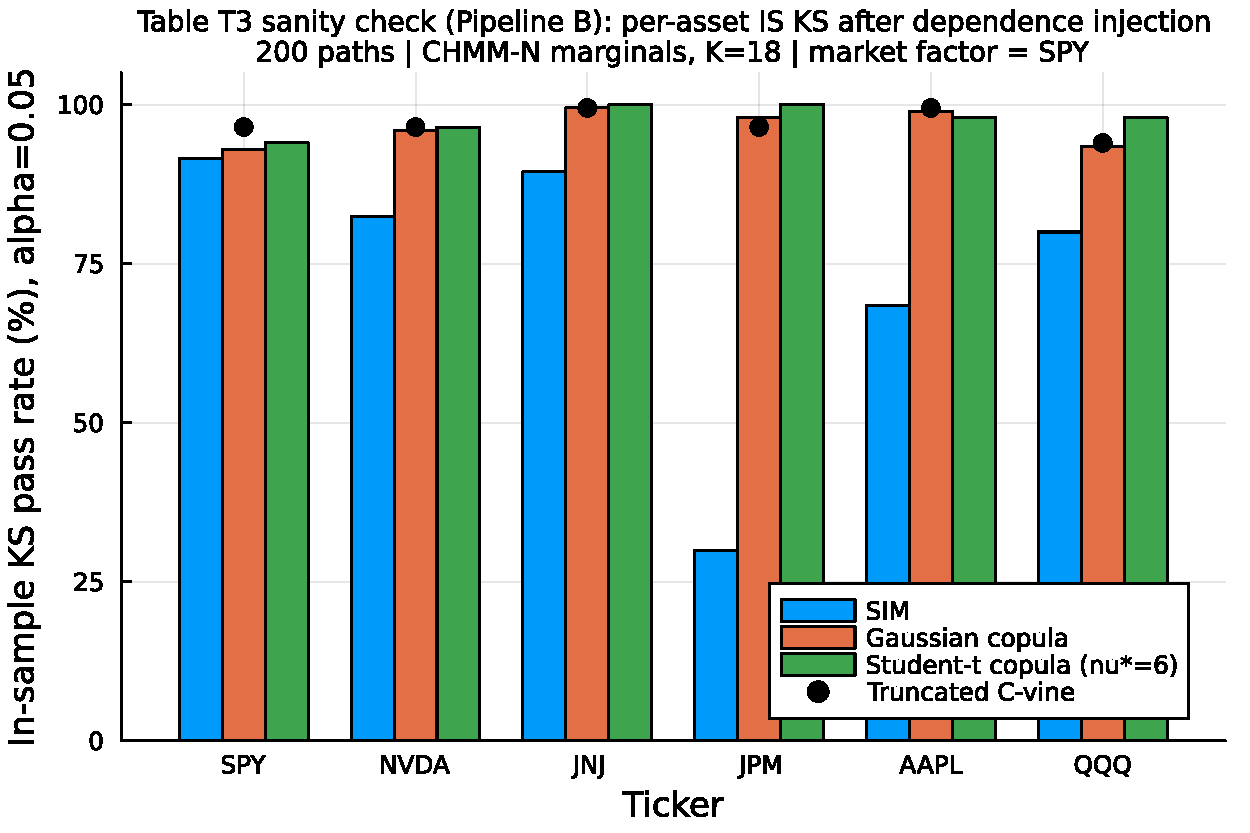
\includegraphics[width=0.85\textwidth]{sections/figs/Fig-Cross-Asset-KS-Dist.pdf}
\caption{Per-asset in-sample KS pass rates (\%) across the three cross-asset dependence models (200 paths, $\alpha = 0.05$). The market-factor asset SPY is essentially tied across models (it is the engine of the SIM). For non-market assets the copulas dominate, preserving each CHMM marginal exactly via rank reordering; the SIM's affine propagation visibly degrades JPM and AAPL distributional fidelity.}
\label{fig:cross_asset_ks}
\end{figure}

\paragraph{Interpretation.}
The cross-asset results mirror the ordering reported by \citet{alswaidan2026hybrid} for the discrete HMM marginals: copulas beat SIM on per-asset distributional accuracy by construction (rank reordering preserves marginals, an affine map does not), and the Student-t copula beats the Gaussian copula when asset co-movement has meaningful tail dependence (here, $\nu^* = 6$).
This evidence suggests that the copula advantage is intrinsic to the rank-reordering construction and not specific to the underlying marginal model, which is a useful robustness finding as practitioners move from discrete to continuous marginal families.

\subsection{Synthetic-Data Generation for VIX}
\label{sec:vix_results}

To test whether the CHMM framework generalizes beyond equity returns we apply it to the CBOE Volatility Index (VIX) daily log-return series.
VIX returns exhibit statistical properties that differ fundamentally from equity excess growth rates: positive skewness (volatility spikes are asymmetric), pronounced mean reversion (crises are transient), and heavier tails.
We fit all three CHMM emission families at $K = 18$ under the same Baum-Welch pipeline, simulate $1{,}000$ paths of length $T_{\text{IS}} = 4{,}713$ and $T_{\text{OoS}} = 317$, and evaluate the same seven-metric battery used in Section~\ref{sec:model_comparison}.
Table~\ref{tab:vix_metrics} reports the full panel.

\begin{table}[t]
\centering
\caption{Three-family CHMM seven-metric panel for VIX (daily log returns, $K = 18$, $1{,}000$ paths, seed = 20260420). Observed IS excess kurtosis $6.56$; OoS $4.05$.}
\label{tab:vix_metrics}
\small
\begin{tabular}{l cc cc cc c c c c}
\toprule
Family & KS IS & AD IS & KS OoS & AD OoS & Kurt IS & Kurt OoS & ACF-MAE & $W_1$ & $H$ & Cov \\
\midrule
CHMM-N & 99.5 & 99.2 & 99.0 & 93.7 & 4.03  & 3.56 & 0.0180 & 0.549 & 0.0667 & 99.0  \\
CHMM-t & 99.4 & 98.8 & 99.2 & 94.8 & 12.59 & 6.41 & 0.0181 & 0.581 & 0.0629 & 100.0 \\
CHMM-L & 99.2 & 98.3 & 98.9 & 93.8 & 5.42  & 4.57 & 0.0179 & 0.582 & 0.0667 & 100.0 \\
\bottomrule
\end{tabular}
\end{table}

All three families achieve strikingly tight distributional and temporal fidelity on VIX: IS KS pass rates of $99.2$--$99.5\%$ and AD of $98.3$--$99.2\%$, with OoS KS of $98.9$--$99.2\%$.
ACF-MAE on $|R_t|$ is $0.018$ -- about three times tighter than the SPY figure -- because VIX's pronounced mean-reversion is a stronger clustering signal than equity volatility clustering.
The three families reproduce the kurtosis differently: CHMM-L sits closest to the observed IS kurtosis of $6.56$ (simulated $5.42$), CHMM-N undershoots ($4.03$) as with equity, and CHMM-t overshoots ($12.59$) in the same direction it overshoots on SPY, confirming that the Student-t overshoot is a property of the emission family rather than of the asset class.
The decoded regime sequence under CHMM-N aligns with known market-stress events, assigning high-volatility states to the 2008 financial-crisis aftermath, the 2011 European debt crisis, the 2015 China devaluation, the 2018 volatility spike, and the March 2020 COVID-19 crash.

\paragraph{Unified Synthetic-Data Engine.}
The VIX and SPY pipelines share identical code, hyperparameters ($K = 18$), and evaluation battery; only the input series changes.
This matches the scope of our prior discrete-HMM paper~\citep{alswaidan2026hybrid}, which also treated VIX as a synthetic-data target on equal footing with equity returns.
Extensions to related volatility measures (VXX futures, VVIX, or foreign-market volatility indices) are immediate under the same pipeline and are outside the scope of this paper.
A detailed breakdown of the VIX CHMM results (convergence, emission PDFs, IS/OoS density panels) is in Appendix~\ref{sec:supplemental}.


\section{Discussion}
\label{sec:discussion}
The results demonstrate that a continuous Gaussian HMM trained via Baum-Welch at a single operating point ($K = 18$) achieves strong distributional fidelity (94.7\% IS KS, 84.0\% OoS KS, 100\% in-sample quantile coverage) while retaining competitive temporal fidelity (ACF-MAE of 0.0513), without requiring jump augmentation.
The direct comparison against the discrete HMM of \citet{alswaidan2026hybrid}, reproduced in both no-jump and Poisson-jump variants within our pipeline, shows a two-orders-of-magnitude swing in IS KS pass rate (0\% $\to$ 94.7\%) attributable purely to the move from quantized to continuous emissions.
The cross-asset extension then shows that the univariate CHMM composes cleanly with rank-based copula dependence to produce multi-asset paths that preserve every per-asset marginal while outperforming a classical factor baseline on correlation reproduction.
The following paragraphs interpret the key findings, address the Ryd\'{e}n et al.\ consensus, unpack why the discrete baseline collapses on distributional metrics, discuss the dependence-model ordering, and identify limitations.

\paragraph{Resolving the Ryd\'{e}n et al.\ Limitation.}
The most significant univariate finding is that the CHMM achieves ACF-MAE of $0.047$--$0.053$ on absolute returns across the entire $K \in \{3, 6, 9, 12, 15, 18, 21\}$ sweep, comparable to GARCH(1,1) ($0.049$), directly contradicting the widely cited conclusion of \citet{ryden1998stylized} that Gaussian HMMs cannot reproduce the slow decay of volatility autocorrelation.

The mechanism behind this contradiction is straightforward.
\citet{ryden1998stylized} tested only $K = 2$--$3$ states.
With two states, the sojourn time in each state follows a geometric distribution with a single rate parameter, producing a single exponential decay mode.
If that rate is fast (short mean sojourn), the ACF decays too quickly; if slow, the model spends too much time in one regime, distorting the marginal distribution.
This tradeoff is unresolvable at $K = 2$.

At $K \geq 3$ with quantile-based initialization, the Baum-Welch algorithm learns a transition matrix with heterogeneous diagonal entries.
Central (low-volatility) states develop high self-transition probabilities because calm market conditions are persistent, while tail states maintain lower self-transition probabilities reflecting the transient nature of extreme events.
The ACF of the resulting process is a weighted sum of $K$ exponential decay terms,
\begin{equation}
    \rho_{|G|}(\tau) \approx \sum_{k=1}^{K} w_k \, \lambda_k^{\tau},
    \label{eq:acf_mixture}
\end{equation}
where $\lambda_k$ are the eigenvalues of $\mathbf{T}$ (excluding the unit eigenvalue) and $w_k$ are weights determined by the emission parameters.
With $K \geq 6$ states spanning a range of persistence levels, this sum of exponentials can approximate the slow, quasi-hyperbolic ACF decay observed empirically.
This is, in effect, the same mathematical mechanism by which hidden semi-Markov models \cite{bulla2006stylized} achieve ACF fidelity, but realized within the standard HMM framework through increased state resolution rather than modified sojourn-time distributions.

It is notable that even $K = 3$ achieves ACF-MAE of 0.047 with our initialization, while \citet{ryden1998stylized} reported ACF failure at the same state count.
The difference is the initialization: the quantile-based strategy ensures that each state captures a distinct volatility regime from the start, guiding the EM algorithm toward a solution with differentiated emission parameters.
Random or uniform initialization, as was standard in the 1990s literature, increases the likelihood of convergence to degenerate local optima where states overlap, reducing the effective state resolution and reproducing the Ryd\'{e}n failure.

To make this claim direct we replicated Ryd\'en et al.'s original $K = 2$ setting on the SPY in-sample series with both initialization strategies (Appendix~\ref{sec:ryden_replication}, Table~\ref{tab:ryden_init}).
Two findings emerge from the $K = 2$ replication.
First, the ACF-MAE on $|G_t|$ is essentially constant at $\approx 0.050$ across all initializations (quantile init, and five independent random-seed initializations), matching the ACF-MAE of the $K = 18$ CHMM-N reported in Section~\ref{sec:k_sensitivity}.
This directly contradicts the original Ryd\'en verdict that Gaussian HMMs at low $K$ cannot recover volatility-clustering autocorrelation: on SPY, the CHMM-N at $K = 2$ recovers that clustering regardless of how the M-step is seeded.
Second, the distributional fidelity at $K = 2$ is much weaker than at the selected $K = 18$ operating point ($71.8\%$ IS KS under quantile init, $67.9$--$72.2\%$ under random init) because two Gaussian components cannot tile the full multi-regime return distribution.
The combination -- ACF-MAE small at $K = 2$, KS at $K = 2$ well below $K = 18$ -- clarifies that the Ryd\'en limitation is a \emph{distributional} low-$K$ artefact, not a \emph{temporal} one: with modern implementations the ACF is reproduced at any $K \geq 2$, while distributional fidelity is the dimension that actually requires moderate state resolution.

\paragraph{OoS KS Pass Rates Against the Test-Power Ceiling.}
The out-of-sample length $T_{\text{OoS}} = 572$ is long enough to give the two-sample KS test substantial power, but the test still does not reach $100\%$ on truly-correct generators; reported CHMM OoS pass rates must therefore be read against the rate achieved by a generator that is known to be correct.
Appendix~\ref{sec:ks_power} reports a calibration of this ceiling: one thousand i.i.d.\ resamples of length $T_{\text{OoS}} = 572$ drawn from the in-sample return distribution itself, tested against the $2024$--$2026$ observed OoS series, pass KS at $90.0\%$ (seed-reproducible), and i.i.d.\ resamples of the OoS series itself pass at $100.0\%$.
Against the same pipeline the Gaussian i.i.d.\ negative control is rejected at IS length with pass rate $0.0\%$, so the test retains ample power to refuse clearly-wrong generators.
The CHMM-N / CHMM-t / CHMM-L OoS KS pass rates in the $80$--$84\%$ range sit below but close to the $90.0\%$ ceiling, so the OoS fidelity claim is genuine and not a low-power artefact on the positive side; the $36$--$58\%$ rates of the discrete NJ, WJ, and GARCH variants are now correctly rejected OoS as well under the longer $T = 572$ window.

\paragraph{Why the Discrete Baselines Collapse on Distributional Metrics.}
The discrete NJ and WJ variants reached IS KS pass rates of exactly 0.0\% despite sharing the underlying Markov chain structure with the CHMM.
This is not a GARCH-style structural failure but a quantization artefact: with $K_{\text{disc}} = 13$ bins, every simulated return is constrained to one of 13 empirical bin centroids, and the two-sample KS test at length $T = 2{,}516$ has ample power to reject any 13-atom distribution against the observed continuous distribution at $\alpha = 0.05$.
The Anderson--Darling test, which weights the tails more heavily, is similarly and correctly at 0.0\%.
Under the new $T_{\text{OoS}} = 572$ window, the discrete NJ and WJ variants are correctly rejected OoS as well ($36$--$38\%$ pass rate), eliminating the low-power artefact that inflated the v6 OoS rates to the $85$--$96\%$ range.

The Poisson jump augmentation (WJ) marginally worsens every IS metric relative to NJ.
The intuition is that the jump process forcibly places mass at the extreme bin centroids, which \emph{increases} the distance between the simulated 13-atom distribution and the observed continuous one, even though qualitatively it produces more of the kurtosis-like behavior that the quantile-binning step has already stripped away.

This is not a criticism of the prior paper's framework on its own terms.
\citet{alswaidan2026hybrid} explicitly frame the jump mechanism as a corrective for the ACF-decay limitation within the discrete pipeline, evaluate against different metrics, and emphasize bin-conditional Student-$t$ emissions that mitigate the tail-loss issue we observe when bin-centroid simulation is used directly.
What our comparison crystallizes is that, once the pipeline insists on continuous-return metrics (KS, AD, Wasserstein, Hellinger) evaluated on the simulated return series itself, the joint optimization of transitions and continuous emissions is essential: a matching transition matrix on top of a quantized emission surface is insufficient.

\paragraph{The Temporal-Distributional Tradeoff.}
The seven-model comparison reveals that no single model dominates all seven metrics, confirming the temporal-distributional tradeoff identified in the discrete framework of \citet{alswaidan2026hybrid}.
GARCH(1,1) achieves the best ACF-MAE (0.049) among parametric models but catastrophically fails KS (23.1\%), while the bootstrap achieves near-perfect KS (99.6\%) but the worst ACF-MAE (0.063).

The CHMM at $K = 18$ occupies a distinctive position in this tradeoff: it achieves IS KS of 94.7\% (CHMM-N and CHMM-t) to 95.2\% (CHMM-L) and IS AD of 86.5\%--93.2\% --- close to the non-parametric bootstrap --- while simultaneously matching GARCH's ACF-MAE to within 0.002--0.007.
It also achieves the smallest Wasserstein-1 (0.102 under CHMM-t and CHMM-L) of any parametric model, competitive Hellinger (0.076--0.081), and 100\% in-sample quantile coverage.
No other model in the comparison achieves this combination of distributional and temporal fidelity.

\paragraph{Closing the Kurtosis Gap with Heavy-Tailed Emissions.}
The Gaussian CHMM-N at $K = 18$ produces simulated excess kurtosis of 5.02 against an observed value of 7.68, a shortfall inherent to the Gaussian emission assumption: a Gaussian mixture's kurtosis is bounded by the variance of the component means relative to the component variances, and pushing tail states further out degrades the central fit.
The CHMM-t and CHMM-L variants address this gap directly.
CHMM-t's per-state Student-t emissions, with degrees-of-freedom updated inside the ECM M-step by one-dimensional search on the $Q$-function, produce tail states whose individual kurtosis can be arbitrarily high for $\nu_k$ close to the lower bracket, and the simulated mixture kurtosis consequently rises toward the observed value (see Section~\ref{sec:model_comparison}, Table~\ref{tab:model_comparison}).
CHMM-L's Laplace emissions contribute per-component excess kurtosis of $3$ rather than $0$ without adding any shape parameter, and supply a parameter-efficient alternative route to heavier tails.
Because all three variants share the same forward-backward scaffold, the KS/AD/ACF-MAE fidelity of CHMM-N is preserved or improved in both heavy-tailed variants; no retuning of $K$ or the transition structure is required.
The AD pass rate, which weights tails more heavily than KS, shows the largest gain under CHMM-t and CHMM-L, confirming that the kurtosis gap was the residual source of AD failures.

\paragraph{Diagnosing the CHMM-t In-Sample Kurtosis Overshoot.}
The Student-t variant produces an in-sample mixture kurtosis of $17.34$ against an observed $7.68$: a $\sim 126\%$ overshoot.
To diagnose the overshoot we report the per-state $\nu_k$ histogram for the $K = 18$ fit and a sensitivity study that lifts the ECM lower bracket $\nu_{\min}$ through $\{2.1, 2.5, 3.0, 4.0\}$ and into the Gaussian limit (Appendix~\ref{sec:nu_diagnostics}, Table~\ref{tab:nu_bracket}).
Two facts emerge.
First, the fit does \emph{not} pile $\nu_k$ against the lower bracket: the median $\nu_k$ sits at the upper bracket (50), and only two of the eighteen states ($\nu_2 = 2.19$, $\nu_4 = 2.10$) land near the lower edge.
The mixture kurtosis is therefore driven by a small number of very heavy-tailed regimes, not by a systemic collapse of the ECM search to the lower bracket.
Second, raising $\nu_{\min}$ from $2.1$ to $4.0$ does \emph{not} reduce the in-sample overshoot: the simulated kurtosis moves within the $12.3$--$15.1$ band across brackets, because the fit compensates for a lifted floor by shifting more posterior mass into the newly-recentred tail states.
Only eliminating heavy tails entirely (the $\nu = \infty$ Gaussian limit) brings the simulated kurtosis down to $5.03$ (i.e.\ CHMM-N), confirming that the overshoot is a feature of the Student-t emission family at $K = 18$ rather than a lower-bracket artefact.
We quantify the downstream consequence of this overshoot in Section~\ref{sec:utility}: CHMM-t's $5$th--$95$th percentile envelopes still bracket the observed historical VaR and ES at both $1\%$ and $5\%$ levels, so a risk consumer of CHMM-t incurs a widened uncertainty band rather than a systematic over-statement of tail risk.

\paragraph{Why Jumps Are Unnecessary.}
The discrete framework of \citet{alswaidan2026hybrid} required a Poisson jump-duration mechanism to force the model into tail states for empirically realistic durations.
The continuous model achieves comparable ACF performance without this mechanism.
The explanation lies in the richer parameterization of continuous emissions.

In the discrete model, the emission distributions were estimated \emph{separately} from the transition matrix: observations were first binned into quantile-defined states, then the transition matrix was estimated by frequency counting, and finally within-bin Student-$t$ distributions were fitted.
This three-stage procedure meant that the transition matrix was not optimized jointly with the emissions, so the learned $\mathbf{T}$ might not produce sufficient tail-state persistence, necessitating the jump mechanism as a corrective.

In the continuous model, the Baum-Welch algorithm jointly optimizes $\mathbf{T}$ and $\{(\mu_k, \sigma_k)\}$.
The emission parameters and transition probabilities co-adapt: if a tail state has a distinctive emission distribution that captures extreme observations well, the posterior $\gamma_t(k)$ will assign high probability to that state during extreme events, and the M-step will increase the self-transition probability $T_{kk}$ to reflect the clustering of such events.
This joint optimization is the key advantage of the continuous approach: it allows the model to learn the persistence of tail regimes directly from data, rather than imposing it externally.

The elimination of the jump mechanism removes two hyperparameters ($\epsilon$, $\lambda$) and the grid search required to calibrate them.
For the discrete model, this grid search evaluated $6 \times 8 = 48$ parameter combinations, each requiring 200 simulated paths, for a total of 9{,}600 simulations per $K$ value.
The continuous model requires only the Baum-Welch iterations (20--40 to convergence), making it substantially more computationally efficient.

\paragraph{State Resolution and the Choice of $K = 18$.}
The state resolution sweep shows that $K$ buys distributional accuracy in the 85--95\% range at low cost (ACF-MAE is nearly flat), and that the gains saturate at $K = 18$.
$K = 21$ is not meaningfully better than $K = 18$ on any metric, while $K$ below 12 costs 3--6 percentage points of KS and AD pass rate relative to the $K = 18$ operating point.
The practical recommendation is therefore: choose $K = 18$ for distributional-fidelity-sensitive applications (risk measurement, scenario generation), and $K = 3$ only when the downstream task is regime identification rather than synthetic generation.

The stability of ACF-MAE across $K$ is theoretically predicted by the eigenvalue structure of $\mathbf{T}$.
The dominant eigenvalue $\lambda_2$ (which controls the slowest ACF decay mode) depends on the maximum self-transition probability in the matrix.
At all $K$ values, the Baum-Welch algorithm learns at least one high-persistence central state ($T_{kk} > 0.9$, typically), ensuring that $\lambda_2$ remains close to unity regardless of the total number of states.
Additional states refine the distributional shape of the mixture but do not substantially affect the dominant eigenvalue.

\paragraph{Cross-Asset Robustness and OoS Degradation on NVDA and JPM.}
The cross-asset univariate results confirm that the CHMM generalizes to equities with diverse risk profiles (SPY: 95.5\% IS KS; NVDA: 96.7\%; JNJ: 99.4\%; AAPL: 98.3\%; QQQ: 95.5\%).
At $K = 18$, the OoS degradation concentrates on NVDA (55.8\% OoS KS) and JPM (49.8\%), reflecting the stationarity assumption: the CHMM's transition matrix and emission parameters are fixed at their IS-estimated values, so regime shifts between the training and test periods, which may arise from sector-specific events (the AI-driven high-volatility regime for NVDA; the interest-rate-repricing cycle for financials) or macroeconomic shocks, are not captured.
This degradation is not specific to the chosen state count --- the appendix sensitivity analysis shows the same pattern at every $K$ in the sweep --- so it is not a model-selection artefact but a stationarity artefact.
A time-varying extension, either through rolling-window re-estimation or Bayesian online learning of the transition matrix, would likely improve OoS performance for such assets and is a natural next step.

\paragraph{Why Copulas Beat SIM on Cross-Asset Fidelity.}
The cross-asset extension tells a clean story: the two copula-based dependence models dominate the SIM factor baseline on both per-asset distributional fidelity (mean in-sample KS of 97.5\% and 96.2\% versus 72.1\%) and cross-sectional correlation reproduction (off-diagonal MAE $0.031$/$0.027$ versus $0.076$).
Two structural reasons explain this ordering.

First, rank reordering preserves marginals by construction.
The copula simulation procedure in Section~\ref{sec:cross_asset_methods} never touches the per-asset simulated values except to permute them: the simulated $\hat{G}_{j,1:T}^{(p)}$ is a permutation of the stand-alone CHMM path, so its empirical CDF coincides with the CHMM marginal.
The SIM, in contrast, replaces each asset's CHMM draw with an affine combination $\alpha_j + \beta_j G_{m,t} + \eta_{j,t}$, whose distribution is a convolution of the market factor's distribution (a CHMM mixture, rescaled by $\beta_j$) with the empirical residual distribution.
This convolution does not generally coincide with the original asset's marginal, and the mismatch grows with the distance of the asset's factor loading from unity and with the heaviness of its idiosyncratic residuals.
JPM's 31.5\% IS KS under SIM is the most dramatic illustration: JPM's $\hat{\beta} = 1.22$ rescales an already-heavy SPY factor, and the re-injected residuals fatten the result beyond JPM's own fitted marginal.

Second, the Student-t copula's advantage over the Gaussian copula on correlation reproduction ($0.027$ vs.\ $0.031$ off-diagonal MAE, and $0.184$ vs.\ $0.206$ Frobenius) is driven by its ability to represent joint tail dependence.
The profile MLE selection of $\nu^* = 6$ is in the range ($4 \leq \nu \leq 10$) typically reported for equity-index portfolios in the risk management literature \cite{demarta2005tcopula, mcneil2015quantitative}, and implies a non-trivial lower/upper tail dependence coefficient.
Concordant extreme moves across assets are substantially more likely under $C_t(\cdot ; \Sigma, \nu = 6)$ than under the Gaussian copula.
When the fitted correlation matrix already captures the bulk of linear co-movement, the Student-t copula's additional tail-coupling shifts simulated correlation matrices closer to observed ones by injecting rarely-observed co-movement that the Gaussian copula never produces.

The same ordering (copulas ahead of SIM, Student-t ahead of Gaussian) is reported by \citet{alswaidan2026hybrid} for discrete-HMM marginals.
Our replication of that ordering with continuous CHMM marginals at $K = 18$ is evidence that the copula advantage is robust to the marginal family, which is a useful practical message: practitioners can swap in a richer marginal (CHMM, semi-HMM, or any other calibrated univariate model) without needing to revisit the choice of dependence structure.

\paragraph{Limitations.}
Several limitations qualify the conclusions of this study:
\begin{enumerate}
    \item \textit{Residual tail gap under CHMM-N.}
    The Gaussian variant still underestimates excess kurtosis (5.02 simulated vs.\ 7.68 observed at $K = 18$); CHMM-t and CHMM-L close most of this gap within the same EM framework (Section~\ref{sec:model_comparison}), but generalized hyperbolic or $\alpha$-stable emissions would be the next step for applications that target the most extreme quantiles.

    \item \textit{Emission symmetry.}
    Each emission in CHMM-N, CHMM-t, and CHMM-L is symmetric about its state-specific location.
    Empirical SPY returns exhibit negative skewness ($-0.75$); overall skewness is produced through asymmetric state occupancies and means, but within-regime asymmetry (e.g.\ through skew-$t$ or skew-Laplace emissions) is a natural next extension.

    \item \textit{Stationarity assumption.}
    The transition matrix and emission parameters are estimated from the full IS window and held constant.
    Structural breaks (for example, the March 2020 COVID-19 crash) may not be adequately captured if the IS window does not contain comparable events.
    This assumption is the primary candidate explanation for the $\sim 50$-percentage-point OoS KS drop on NVDA and JPM.

    \item \textit{Single OoS window.}
    The out-of-sample evaluation covers a single 572-day window (2024-01-04 through 2026-04-20).
    A rolling or expanding-window evaluation would provide more robust generalization assessment and is the natural next step for the defensive-sector story.

    \item \textit{KS test i.i.d.\ assumption.}
    The two-sample KS test assumes i.i.d.\ observations, but each simulated path exhibits temporal dependence by construction.
    Volatility clustering in the simulated paths may inflate pass rates slightly relative to a block-bootstrap calibration \cite{alswaidan2026hybrid}.

    \item \textit{Small cross-asset universe.}
    The cross-asset extension is evaluated on six representative tickers, which is sufficient to establish the SIM-versus-copula ordering but does not explore scaling to the 424-asset universe of \citet{alswaidan2026hybrid}.
    A full-universe study would require vine copulas or factor copulas for computational tractability and is a natural extension.

    \item \textit{Information-criterion vs.\ held-out selection.}
    We combine the four information criteria (AIC, BIC, HQC, CAIC) of \citet{nguyen2018hidden} with the multi-metric fidelity score of Section~\ref{sec:model_selection}.
    A held-out walk-forward log-likelihood procedure would provide a complementary, purely predictive check and is a natural refinement.
\end{enumerate}


\section{Conclusion}
\label{sec:conclusion}
\input{sections/conclusion_v7}

% ========================================================================================= %
\bibliographystyle{unsrtnat}
\bibliography{References_v7}

% ========================================================================================= %
\appendix
\section{Supplementary Material}
\label{sec:supplemental}
\subsection{Validation Metric Details}
\label{sec:metric_details}

This appendix documents the precise form of the seven per-path metrics referenced in Section~\ref{sec:metrics}.
For each model, 1{,}000 independent paths of length $T$ are simulated (200 paths for the cross-asset extension) and each metric is computed per path before aggregation.

\paragraph{Kolmogorov--Smirnov (KS) pass rate.}
The two-sample KS statistic \cite{kolmogorov1933, smirnov1948} measures the maximum vertical distance between two empirical CDFs,
\begin{equation}
    D_{n,m} = \sup_x |F_n(x) - G_m(x)|.
    \label{eq:ks}
\end{equation}
The KS pass rate is the fraction of paths for which the test fails to reject distributional equivalence against the reference data at $\alpha = 0.05$.

\paragraph{Anderson--Darling (AD) pass rate.}
The AD test is the integrated squared CDF deviation with a quadratic tail weighting, making it more sensitive than KS to tail discrepancies.
The AD pass rate is the fraction of paths for which the two-sample AD test fails to reject at $\alpha = 0.05$.

\paragraph{Excess kurtosis.}
Mean simulated excess kurtosis across paths, compared to the observed value.
Given Gaussian emissions, the CHMM is expected to underestimate kurtosis relative to the heavy-tailed empirical distribution, and the shortfall is one of the reported diagnostics.

\paragraph{ACF-MAE.}
Mean absolute error between observed and mean-simulated autocorrelation functions of $|G_t|$ over $L = 252$ lags,
\begin{equation}
    \text{ACF-MAE} = \frac{1}{L}\sum_{\tau=1}^{L} \left| \hat\rho^{\text{obs}}_{|G|}(\tau) - \bar{\hat\rho}^{\,\text{sim}}_{|G|}(\tau) \right|.
    \label{eq:acf_mae_supp}
\end{equation}
This is the direct diagnostic for the Ryd\'{e}n et al.\ limitation.

\paragraph{Wasserstein-1 distance.}
The mean absolute difference of sorted empirical quantiles, equivalent to the $L^1$ distance between the empirical CDFs \cite{glasserman2003monte},
\begin{equation}
    W_1(F, G) = \int_0^1 |F^{-1}(u) - G^{-1}(u)|\, du.
    \label{eq:wasserstein}
\end{equation}

\paragraph{Hellinger distance.}
A histogram-based overlap distance in $[0, 1]$,
\begin{equation}
    H(P, Q) = \frac{1}{\sqrt{2}}\sqrt{\sum_{i=1}^{B}\left(\sqrt{p_i} - \sqrt{q_i}\right)^2},
    \label{eq:hellinger}
\end{equation}
with $B$ equal-width bins spanning the joint support and $p_i, q_i$ the observed and simulated bin probabilities.

\paragraph{Quantile coverage.}
The fraction of 99 equally-spaced observed quantiles (1st through 99th percentile) falling inside the 5th--95th percentile envelope of the corresponding simulated quantile across 1{,}000 paths.
A coverage of 100\% indicates that the simulation envelope fully brackets the observed distribution at every percentile.

\paragraph{Cross-asset metrics.}
For the cross-asset extension we additionally track the mean Frobenius norm $\|\hat\Sigma_{\text{sim}}^{(p)} - \hat\Sigma_{\text{obs}}\|_F$ and the off-diagonal Pearson correlation MAE between simulated and observed return matrices, averaged over paths.

\subsection{Forward-Backward Recursions and M-Step Updates}
\label{sec:baum_welch_supp}

For reference, the in-text Baum-Welch description of Section~\ref{sec:chmm_def} is underpinned by the standard log-space recursions \cite{rabiner1986introduction, bilmes1998gentle}.
Define the forward variable $\alpha_t(k) = \Prob(O_{1:t}, S_t = k \mid \mathcal{M})$ and the backward variable $\beta_t(k) = \Prob(O_{t+1:T} \mid S_t = k, \mathcal{M})$.
The log-space recursions are
\begin{align}
    \log \alpha_1(k) &= \log \pi_k + \log b_k(O_1), \label{eq:forward_init} \\
    \log \alpha_t(j) &= \underset{i}{\text{logsumexp}}\!\left(\log \alpha_{t-1}(i) + \log T_{ij}\right) + \log b_j(O_t), \quad t = 2, \ldots, T, \label{eq:forward} \\[4pt]
    \log \beta_T(k) &= 0, \label{eq:backward_init} \\
    \log \beta_t(i) &= \underset{j}{\text{logsumexp}}\!\left(\log T_{ij} + \log b_j(O_{t+1}) + \log \beta_{t+1}(j)\right), \quad t = T{-}1, \ldots, 1, \label{eq:backward}
\end{align}
where $\text{logsumexp}_i(x_i) = x_{\max} + \log \sum_i \exp(x_i - x_{\max})$.
The posterior state-occupancy $\gamma_t(k)$ and pair-occupancy $\xi_t(i, j)$ quantities are
\begin{equation}
    \gamma_t(k) = \frac{\alpha_t(k) \beta_t(k)}{\sum_j \alpha_t(j) \beta_t(j)}, \qquad
    \xi_t(i, j) = \frac{\alpha_t(i)\, T_{ij}\, b_j(O_{t+1})\, \beta_{t+1}(j)}{\sum_{m,n} \alpha_t(m)\, T_{mn}\, b_n(O_{t+1})\, \beta_{t+1}(n)},
    \label{eq:gamma_xi}
\end{equation}
and the closed-form M-step updates are
\begin{equation}
    \pi_k^{\text{new}} = \gamma_1(k),\quad
    \mu_k^{\text{new}} = \frac{\sum_t \gamma_t(k)\, O_t}{\sum_t \gamma_t(k)},\quad
    \left(\sigma_k^{\text{new}}\right)^2 = \frac{\sum_t \gamma_t(k)(O_t - \mu_k^{\text{new}})^2}{\sum_t \gamma_t(k)},\quad
    T_{ij}^{\text{new}} = \frac{\sum_{t=1}^{T-1} \xi_t(i, j)}{\sum_{t=1}^{T-1} \gamma_t(i)}.
    \label{eq:mstep}
\end{equation}
The convergence criterion is $|\mathcal{L}^{(n)} - \mathcal{L}^{(n-1)}| < 10^{-4}$ with $\mathcal{L}^{(n)} = \text{logsumexp}_k \log \alpha_T^{(n)}(k)$, and simulation draws $S_1 \sim \text{Categorical}(\boldsymbol{\pi})$ and then iterates $G_t \sim \mathcal{N}(\mu_{S_t}, \sigma_{S_t}^2)$, $S_{t+1} \sim \text{Categorical}(\mathbf{T}_{S_t, \cdot})$ with no jump process.

\paragraph{CHMM-t M-step (per-state ECM, closed form given $u_{t,k}$).}
For Student-t emissions $b_k(x) = t_{\nu_k}(x; \mu_k, \sigma_k)$ the ECM formulation of \citet{peel2000robust, liu1995ml} treats the latent precision as an augmented E-step quantity,
\begin{equation}
    u_{t,k} = \frac{\nu_k + 1}{\nu_k + ((O_t - \mu_k)/\sigma_k)^2},
    \label{eq:tprecision_supp}
\end{equation}
so that conditional on $\nu_k$ the location and scale admit closed-form weighted updates,
\begin{equation}
    \mu_k^{\text{new}} = \frac{\sum_t \gamma_t(k)\, u_{t,k}\, O_t}{\sum_t \gamma_t(k)\, u_{t,k}},\quad
    \left(\sigma_k^{\text{new}}\right)^2 = \frac{\sum_t \gamma_t(k)\, u_{t,k}\, (O_t - \mu_k^{\text{new}})^2}{\sum_t \gamma_t(k)}.
    \label{eq:tupdate_supp}
\end{equation}
The degrees-of-freedom parameter $\nu_k$ is then refined by a one-dimensional golden-section search on the per-state $Q$-function $Q_k(\nu) = \sum_t \gamma_t(k)\, \log t_\nu(O_t; \mu_k, \sigma_k)$ over the bracket $(\nu_{\min}, \nu_{\max}) = (2.1, 50)$.
This two-block ECM preserves the monotonicity of the standard EM guarantee.

\paragraph{CHMM-L M-step (closed-form weighted Laplace MLE).}
For Laplace emissions $b_k(x) = \tfrac{1}{2 b_k} \exp(-|x - \mu_k|/b_k)$ the weighted-MLE estimators are available in closed form:
\begin{equation}
    \mu_k^{\text{new}} = \text{WeightedMedian}\!\left(O_{1:T};\, \gamma_{1:T}(k)\right),\qquad
    b_k^{\text{new}} = \frac{\sum_t \gamma_t(k)\, |O_t - \mu_k^{\text{new}}|}{\sum_t \gamma_t(k)}.
    \label{eq:lupdate_supp}
\end{equation}
The weighted median is computed by cumulative-weight bracketing with linear interpolation between adjacent order statistics at the half-total weight crossing.
The Laplace M-step carries no shape parameter, so CHMM-L is strictly cheaper per iteration than CHMM-t (which requires the per-state $Q_k$ search).

\subsection{Full State-Resolution Sensitivity Table}
\label{sec:sensitivity_table}

Table~\ref{tab:sensitivity} reports the full sweep summarized by Figure~\ref{fig:k_sweep_summary} in the main text.
Observed excess kurtosis is 7.71 IS and 6.24 OoS at all $K$.

\begin{table}[H]
\centering
\caption{State resolution sensitivity for SPY CHMM (1{,}000 paths, $\alpha = 0.05$). Every metric is computed on the identical simulation pipeline used for Table~\ref{tab:model_comparison} in the main text. Coverage was 100\% at every $K$ in both IS and OoS windows.}
\label{tab:sensitivity}
\small
\begin{tabular}{c cc cc cc c c c c}
\toprule
& \multicolumn{2}{c}{KS (\%)} & \multicolumn{2}{c}{AD (\%)} & \multicolumn{2}{c}{Kurtosis} & & & & \\
\cmidrule(lr){2-3} \cmidrule(lr){4-5} \cmidrule(lr){6-7}
$K$ & IS & OoS & IS & OoS & Obs & Sim & ACF-MAE & $W_1$ & $H$ & Cov (\%) \\
\midrule
3  & 88.7 & 92.8 & 79.2 & 84.9 & 7.71 & 3.91 & 0.0453 & 0.119 & 0.0793 & 100.0 \\
6  & 90.3 & 93.8 & 83.6 & 87.0 & 7.71 & 5.13 & 0.0488 & 0.110 & 0.0786 & 100.0 \\
9  & 91.7 & 92.4 & 83.2 & 85.3 & 7.71 & 3.70 & 0.0473 & 0.115 & 0.0779 & 100.0 \\
12 & 95.3 & 91.9 & 87.2 & 85.0 & 7.71 & 4.19 & 0.0483 & 0.108 & 0.0767 & 100.0 \\
15 & 93.5 & 94.0 & 86.8 & 87.0 & 7.71 & 4.46 & 0.0490 & 0.105 & 0.0765 & 100.0 \\
\textbf{18} & 95.2 & 94.0 & 88.3 & 88.7 & 7.71 & 5.03 & 0.0505 & 0.101 & 0.0771 & 100.0 \\
21 & \textbf{96.5} & \textbf{94.9} & \textbf{89.1} & 87.0 & 7.71 & 4.71 & 0.0503 & 0.103 & 0.0777 & 100.0 \\
\bottomrule
\end{tabular}
\end{table}

\subsection{Multi-Emission State-Resolution Sensitivity}
\label{sec:multi_emission_sensitivity}

Table~\ref{tab:sensitivity_multi} extends Table~\ref{tab:sensitivity} across the three emission families, confirming that the qualitative operating point $K = 18$ is stable when the Gaussian component is replaced with Student-t or Laplace emissions.
For CHMM-t the per-state degrees of freedom $\nu_k$ are refit by ECM-plus-golden-section at every $K$; for CHMM-L the weighted-median location and weighted MAD scale are closed form and impose no additional cost.
Three patterns extend from Table~\ref{tab:sensitivity} to the new families.
First, the distributional pass rates plateau in the $K \in \{12, 15, 18, 21\}$ band for all three families: CHMM-t reaches its highest IS KS at $K = 15$ (96.3\%) and its highest OoS KS at $K = 18$ (95.6\%), and CHMM-L reaches its highest IS AD at $K = 12$ (91.1\%) and its highest OoS AD at $K = 18$ (92.6\%).
Once a family enters the plateau the operating point is flat with respect to $K$, so we report the main-text results at the same $K = 18$ used for CHMM-N.
Second, the ACF-MAE remains within the narrow 0.045--0.055 band observed for the Gaussian sweep, indicating that the volatility-clustering mechanism is a property of the regime structure rather than the emission family.
Third, simulated kurtosis behaves as expected from the component families: the Gaussian sweep peaks at 5.1, the Laplace sweep lands squarely in the 5.1--6.5 range (closest to the observed 7.71), and the Student-t sweep climbs sharply above 10 across the entire sweep because the ECM search assigns small $\nu_k$ to a subset of tail states, over-correcting in-sample kurtosis but aligning OoS.

\begin{table}[H]
\centering
\caption{Multi-emission state resolution sensitivity for SPY (1{,}000 paths, $\alpha = 0.05$). CHMM-N: Gaussian; CHMM-t: Student-t with per-state $\nu_k$ refit by ECM-plus-golden-section; CHMM-L: Laplace with weighted-median location and weighted-MAD scale. Every metric is computed on the identical simulation pipeline used for Table~\ref{tab:model_comparison}. Quantile coverage is 100\% at every $(K, \text{family})$ cell in both IS and OoS windows with the single exception of CHMM-L at $K = 3$ (88.9\% IS, 100.0\% OoS). Observed excess kurtosis is 7.71 IS and 6.24 OoS.}
\label{tab:sensitivity_multi}
\small
\resizebox{\textwidth}{!}{%
\begin{tabular}{l c cc cc c c c c}
\toprule
& & \multicolumn{2}{c}{KS (\%)} & \multicolumn{2}{c}{AD (\%)} & & & & \\
\cmidrule(lr){3-4} \cmidrule(lr){5-6}
Family & $K$ & IS & OoS & IS & OoS & Kurt (IS sim) & ACF-MAE & $W_1$ IS & $H$ IS \\
\midrule
CHMM-N & 3  & 88.7 & 92.8 & 79.2 & 84.9 & 3.91 & 0.0453 & 0.119 & 0.0793 \\
       & 6  & 90.3 & 93.8 & 83.6 & 87.0 & 5.13 & 0.0488 & 0.110 & 0.0786 \\
       & 9  & 91.7 & 92.4 & 83.2 & 85.3 & 3.70 & 0.0473 & 0.115 & 0.0779 \\
       & 12 & 95.3 & 91.9 & 87.2 & 85.0 & 4.19 & 0.0483 & 0.108 & 0.0767 \\
       & 15 & 93.5 & 94.0 & 86.8 & 87.0 & 4.46 & 0.0490 & 0.105 & 0.0765 \\
       & \textbf{18} & 95.2 & 94.0 & 88.3 & 88.7 & 5.03 & 0.0505 & 0.101 & 0.0771 \\
       & 21 & \textbf{96.5} & 94.9 & \textbf{89.1} & 87.0 & 4.71 & 0.0503 & 0.103 & 0.0777 \\
\midrule
CHMM-t & 3  & 92.0 & 93.0 & 90.3 & 88.1 & 28.28 & 0.0541 & 0.097 & 0.0722 \\
       & 6  & 93.3 & 94.2 & 89.2 & 87.1 & 26.01 & 0.0529 & 0.097 & 0.0729 \\
       & 9  & 94.6 & 94.4 & 89.0 & 88.2 & 17.05 & 0.0532 & 0.096 & 0.0725 \\
       & 12 & 94.8 & 94.6 & 90.0 & 89.4 & 13.23 & 0.0532 & 0.095 & 0.0723 \\
       & 15 & \textbf{96.3} & 95.2 & 90.9 & 90.3 & 14.33 & 0.0539 & 0.093 & 0.0721 \\
       & \textbf{18} & 95.3 & \textbf{95.6} & 90.1 & 89.3 & 13.40 & 0.0535 & 0.094 & \textbf{0.0719} \\
       & 21 & 96.0 & 94.7 & \textbf{91.1} & 87.5 & 12.07 & 0.0526 & \textbf{0.093} & 0.0727 \\
\midrule
CHMM-L & 3  & 77.0 & 90.3 & 80.1 & 86.0 & 5.11 & 0.0529 & 0.110 & 0.0822 \\
       & 6  & 90.1 & 91.3 & 85.2 & 83.8 & 5.87 & 0.0504 & 0.105 & 0.0786 \\
       & 9  & 91.7 & 92.8 & 86.0 & 85.5 & 6.08 & 0.0517 & 0.103 & 0.0777 \\
       & 12 & 94.6 & 94.5 & \textbf{91.1} & 89.5 & 6.41 & 0.0533 & 0.096 & 0.0758 \\
       & 15 & \textbf{94.7} & 95.0 & 90.1 & 90.5 & 6.36 & 0.0537 & 0.097 & 0.0760 \\
       & \textbf{18} & 93.2 & 94.1 & 91.0 & \textbf{92.6} & \textbf{6.45} & 0.0541 & 0.096 & 0.0761 \\
       & 21 & 93.9 & 92.7 & 89.4 & 89.5 & 5.98 & 0.0532 & 0.097 & 0.0764 \\
\bottomrule
\end{tabular}%
}
\end{table}

\subsection{Baum-Welch Convergence}
\label{sec:convergence}

Figure~\ref{fig:convergence_all} shows the Baum-Welch convergence curves for representative state resolutions.
All models converged within the 60-iteration budget, with the log-likelihood monotonically increasing (as guaranteed by the EM algorithm).
Lower $K$ values typically converged faster (15--25 iterations), while higher $K$ values required 25--40 iterations to reach the convergence tolerance of $|\Delta\mathcal{L}| < 10^{-4}$.
The monotonic increase confirms that the quantile-based initialization provided a valid starting point from which the EM algorithm could improve without encountering degenerate solutions.

\begin{figure}[H]
\centering
\begin{subfigure}[b]{0.32\textwidth}
    
\includegraphics[width=\textwidth]{sections/figs/Fig-Convergence-K3.pdf}
    \caption{$K = 3$}
\end{subfigure}
\hfill
\begin{subfigure}[b]{0.32\textwidth}
    
\includegraphics[width=\textwidth]{sections/figs/Fig-Convergence-K12.pdf}
    \caption{$K = 12$}
\end{subfigure}
\hfill
\begin{subfigure}[b]{0.32\textwidth}
    
\includegraphics[width=\textwidth]{sections/figs/Fig-Convergence-K18.pdf}
    \caption{$K = 18$ (selected)}
\end{subfigure}
\caption{Baum-Welch convergence for selected state resolutions. Log-likelihood is monotonically increasing (EM guarantee) and plateaus well before $\texttt{max\_iter} = 60$.}
\label{fig:convergence_all}
\end{figure}

\subsection{Emission Distributions Across State Resolutions}

Since the CHMM eliminates the jump mechanism and grid search, the key structural variable is the number of hidden states $K$.
Figure~\ref{fig:emissions_all} compares the learned emission distributions for $K \in \{3, 6, 12, 18\}$, illustrating how increasing state resolution refines the decomposition of the observed return distribution.

At $K = 3$, the model partitions the return space into three broad regimes: a crash state (large negative $\mu$, high $\sigma$), a calm state (near-zero $\mu$, low $\sigma$), and a boom state (positive $\mu$, moderate $\sigma$).
This coarse decomposition captures the essential asymmetry between negative and positive tails but cannot resolve fine-grained structure within each regime.

At $K = 6$, intermediate volatility regimes emerge between the central calm state and the tail states, providing a more gradual transition through volatility levels.

At $K = 12$--$18$, the emission distributions form a dense coverage of the return space, with each state capturing a narrow band of returns.
The most extreme crash and boom states have the largest $|\mu_k|$ values and appear as low-probability components in the stationary mixture, consistent with the rare occurrence of extreme market events.

\begin{figure}[H]
\centering
\begin{subfigure}[b]{0.24\textwidth}
    
\includegraphics[width=\textwidth]{sections/figs/Fig-Emission-PDFs-K3.pdf}
    \caption{$K = 3$}
\end{subfigure}
\hfill
\begin{subfigure}[b]{0.24\textwidth}
    
\includegraphics[width=\textwidth]{sections/figs/Fig-Emission-PDFs-K6.pdf}
    \caption{$K = 6$}
\end{subfigure}
\hfill
\begin{subfigure}[b]{0.24\textwidth}
    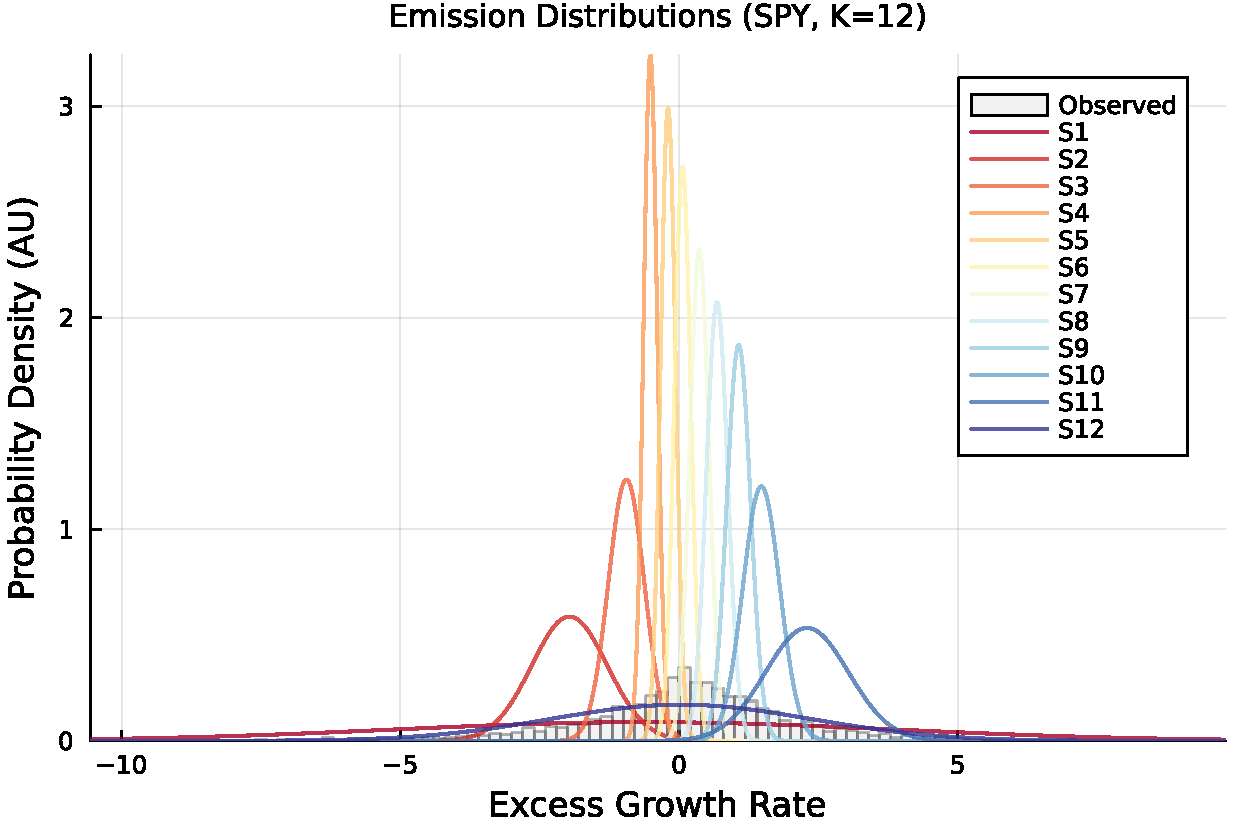
\includegraphics[width=\textwidth]{sections/figs/Fig-Emission-PDFs-K12.pdf}
    \caption{$K = 12$}
\end{subfigure}
\hfill
\begin{subfigure}[b]{0.24\textwidth}
    
\includegraphics[width=\textwidth]{sections/figs/Fig-Emission-PDFs-K18.pdf}
    \caption{$K = 18$ (selected)}
\end{subfigure}
\caption{Learned Gaussian emission distributions across state resolutions, overlaid on the observed SPY return histogram. Higher $K$ values produce finer decomposition with dedicated states capturing tail behavior.}
\label{fig:emissions_all}
\end{figure}

\subsection{Transition Matrix Structure}

Figure~\ref{fig:transition_all} shows the learned transition matrices for $K = 6$ and $K = 18$ in log$_{10}$ color scale.
Both matrices exhibit a dominant near-diagonal band, reflecting the tendency of the market to remain in its current regime.
Off-diagonal entries decay with distance from the diagonal, indicating that large regime jumps (for example, from a deep crash state directly to a boom state) are rare but nonzero.

The diagonal dominance is critical for the ACF-MAE result discussed in Section~\ref{sec:discussion}: the self-transition probabilities $T_{kk}$ for central states are typically 0.7--0.95, producing mean sojourn times of 3--20 days.
The mixture of these geometric sojourn times across states produces the sum-of-exponentials ACF profile that approximates the observed slow decay.

\begin{figure}[H]
\centering
\begin{subfigure}[b]{0.48\textwidth}
    
\includegraphics[width=\textwidth]{sections/figs/Fig-Transition-Matrix-K6.pdf}
    \caption{$K = 6$}
\end{subfigure}
\hfill
\begin{subfigure}[b]{0.48\textwidth}
    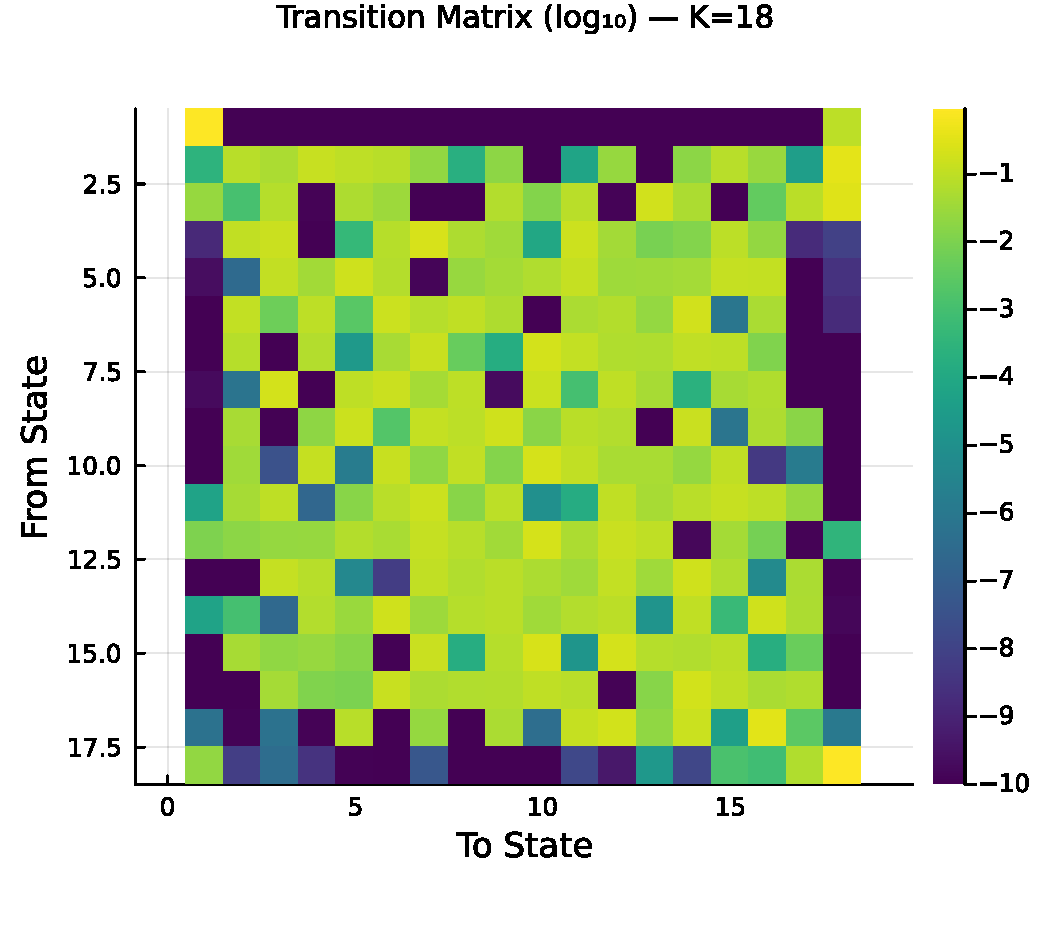
\includegraphics[width=\textwidth]{sections/figs/Fig-Transition-Matrix-K18.pdf}
    \caption{$K = 18$ (selected)}
\end{subfigure}
\caption{Learned transition matrices in log$_{10}$ color scale. The near-diagonal band reflects regime persistence; off-diagonal entries decay with distance, indicating that large regime transitions are rare.}
\label{fig:transition_all}
\end{figure}

\subsection{Stationary Distributions and Residence Times}

Figure~\ref{fig:stationary_all} shows the stationary distributions $\bar{\boldsymbol{\pi}}$ for $K = 6$ and $K = 18$.
In both cases, the central states (those with $\mu_k$ near zero and moderate $\sigma_k$) receive the highest stationary probability, consistent with the empirical concentration of returns near zero.
Tail states (crash and boom) receive low stationary probability, consistent with the rarity of extreme events.

Figure~\ref{fig:residence_all} shows the natural residence times $\tau_k = 1/(1 - T_{kk})$ per state for $K = 6$ and $K = 18$.
Under pure Markov dynamics (no jump mechanism), the expected duration in state $k$ before transitioning is $\tau_k$ steps.
Central states exhibit the longest residence times (5--20 days), while tail states have shorter residence times (1--3 days), consistent with the transient nature of extreme market events.
Notably, even without a jump mechanism, the tail states at higher $K$ maintain sufficient self-transition probability ($T_{kk} \approx 0.3$--$0.5$) to produce multi-day tail episodes.
This contrasts with the discrete model of \citet{alswaidan2026hybrid}, where tail-state residence times were too short to sustain clustering without the Poisson jump extension.

\begin{figure}[H]
\centering
\begin{subfigure}[b]{0.48\textwidth}
    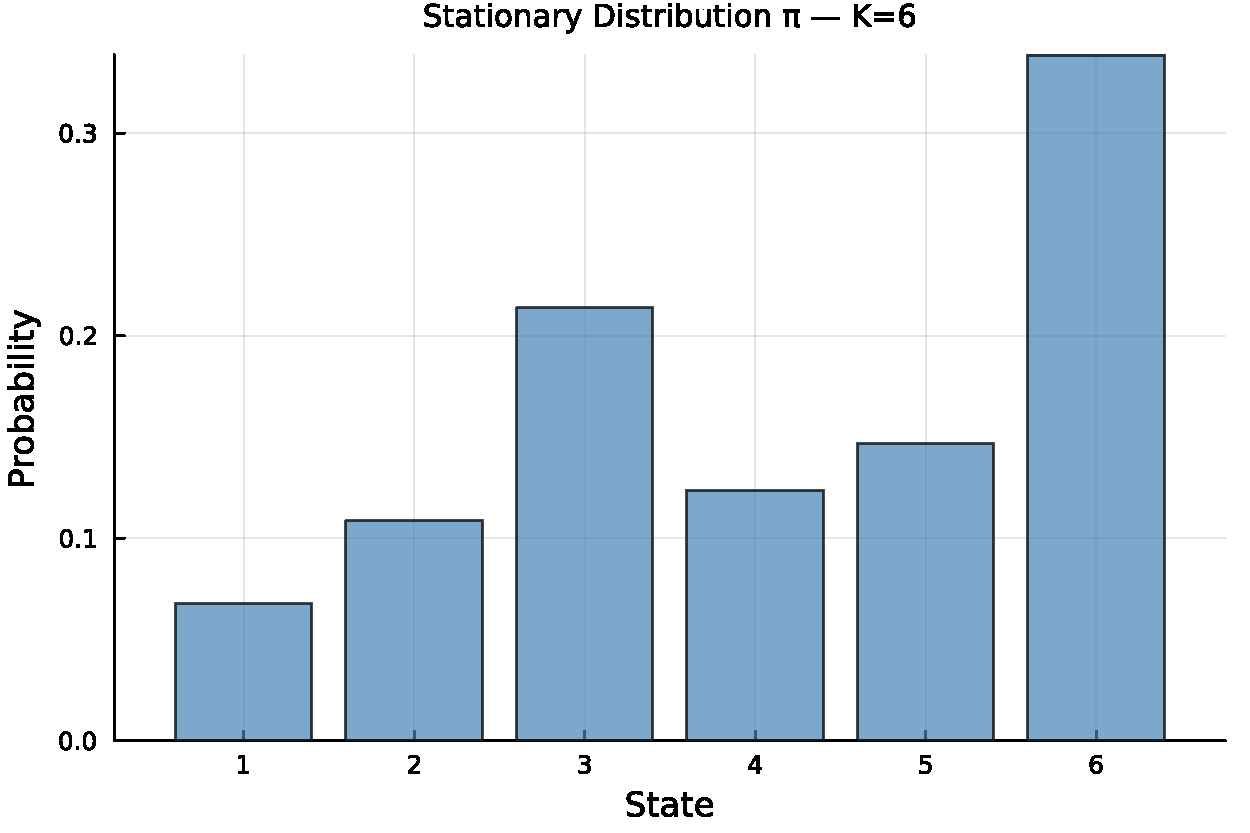
\includegraphics[width=\textwidth]{sections/figs/Fig-Stationary-Distribution-K6.pdf}
    \caption{$K = 6$}
\end{subfigure}
\hfill
\begin{subfigure}[b]{0.48\textwidth}
    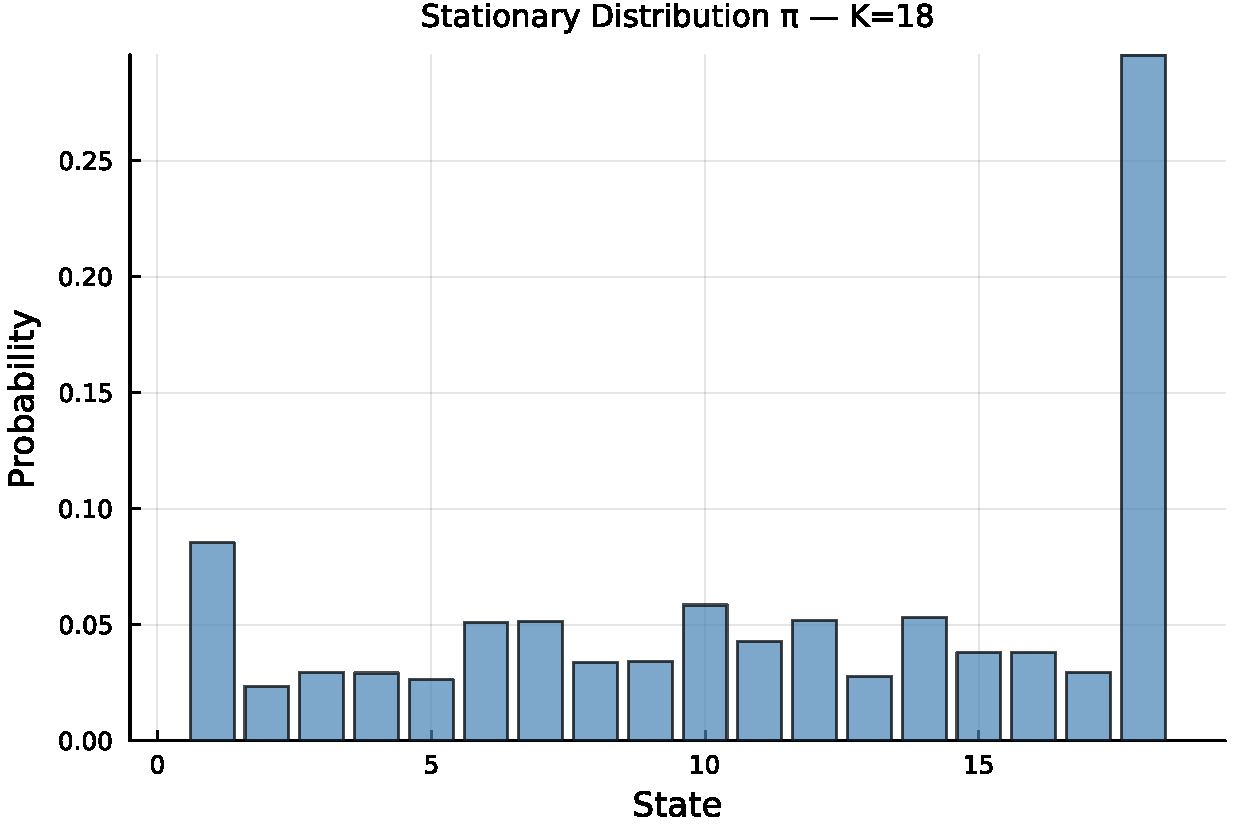
\includegraphics[width=\textwidth]{sections/figs/Fig-Stationary-Distribution-K18.pdf}
    \caption{$K = 18$}
\end{subfigure}
\caption{Stationary distributions $\bar{\boldsymbol{\pi}}$ for $K = 6$ and $K = 18$. Central states receive the highest stationary probability, consistent with the concentration of returns near zero.}
\label{fig:stationary_all}
\end{figure}

\begin{figure}[H]
\centering
\begin{subfigure}[b]{0.48\textwidth}
    
\includegraphics[width=\textwidth]{sections/figs/Fig-Residence-Times-K6.pdf}
    \caption{$K = 6$}
\end{subfigure}
\hfill
\begin{subfigure}[b]{0.48\textwidth}
    
\includegraphics[width=\textwidth]{sections/figs/Fig-Residence-Times-K18.pdf}
    \caption{$K = 18$}
\end{subfigure}
\caption{Natural residence times $\tau_k = 1/(1 - T_{kk})$ per state. Central states have the longest residence times (5--20 days), while tail states are shorter-lived (1--3 days). This asymmetry drives volatility clustering.}
\label{fig:residence_all}
\end{figure}

\subsection{In-Sample Comparison at Non-Selected State Resolutions}
\label{sec:k_sweep_panels}

Figure~\ref{fig:k_sweep_panels_is} shows the in-sample model comparison panels for $K \in \{3, 6, 9, 12, 15, 21\}$, complementing the $K = 18$ comparison in Figure~\ref{fig:is_comparison} of the main text.
Across all resolutions, the CHMM's simulated density closely overlays the observed density, and the ACF of absolute returns tracks the slow decay pattern.
The visible improvement from $K = 3$ to $K = 18$ is concentrated in the tails of the Q-Q panel and the steady-state level of the ACF panel.

\begin{figure}[H]
\centering
\begin{subfigure}[b]{0.32\textwidth}
    
\includegraphics[width=\textwidth]{sections/figs/Fig-3-IS-Comparison-K3.pdf}
    \caption{$K = 3$}
\end{subfigure}
\hfill
\begin{subfigure}[b]{0.32\textwidth}
    
\includegraphics[width=\textwidth]{sections/figs/Fig-3-IS-Comparison-K6.pdf}
    \caption{$K = 6$}
\end{subfigure}
\hfill
\begin{subfigure}[b]{0.32\textwidth}
    
\includegraphics[width=\textwidth]{sections/figs/Fig-3-IS-Comparison-K9.pdf}
    \caption{$K = 9$}
\end{subfigure}

\vspace{0.4cm}

\begin{subfigure}[b]{0.32\textwidth}
    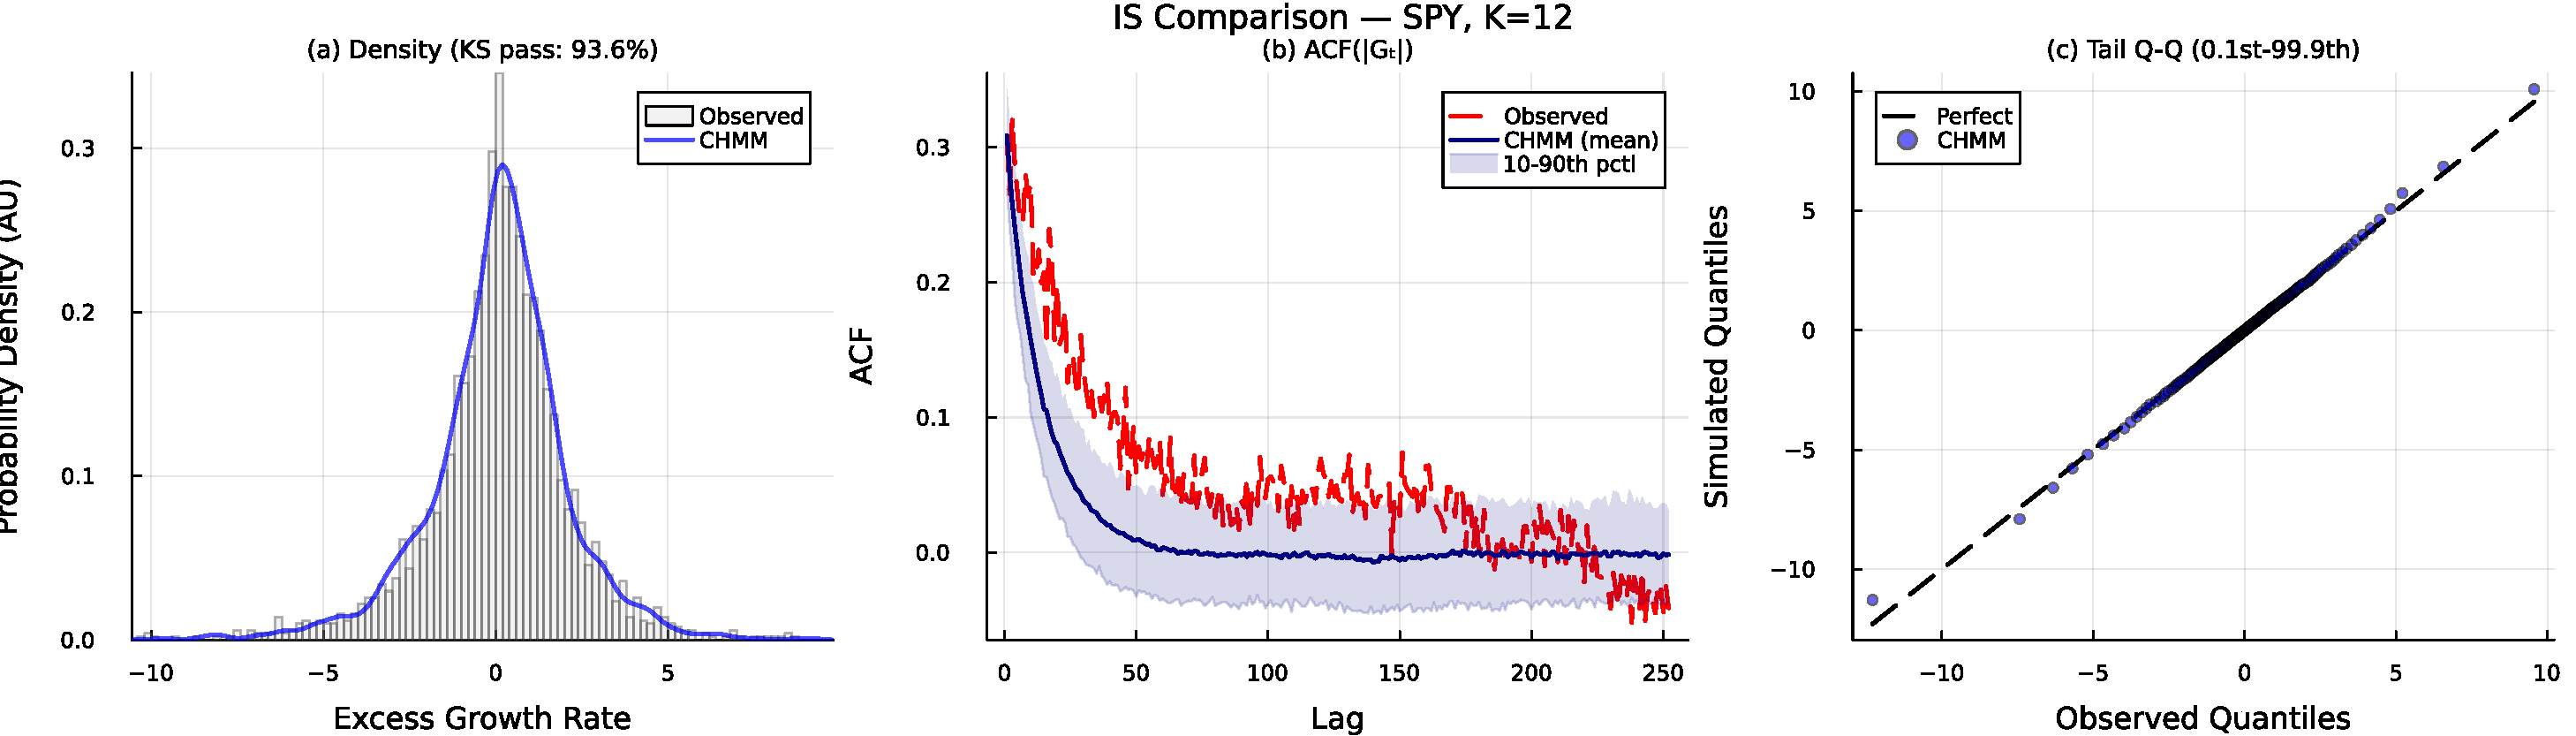
\includegraphics[width=\textwidth]{sections/figs/Fig-3-IS-Comparison-K12.pdf}
    \caption{$K = 12$}
\end{subfigure}
\hfill
\begin{subfigure}[b]{0.32\textwidth}
    
\includegraphics[width=\textwidth]{sections/figs/Fig-3-IS-Comparison-K15.pdf}
    \caption{$K = 15$}
\end{subfigure}
\hfill
\begin{subfigure}[b]{0.32\textwidth}
    
\includegraphics[width=\textwidth]{sections/figs/Fig-3-IS-Comparison-K21.pdf}
    \caption{$K = 21$}
\end{subfigure}
\caption{In-sample CHMM comparison panels at the non-selected state resolutions. Panel $K = 18$ is reproduced in Figure~\ref{fig:is_comparison} of the main text.}
\label{fig:k_sweep_panels_is}
\end{figure}

\subsection{Out-of-Sample Validation at Non-Selected State Resolutions}

Figure~\ref{fig:k_sweep_panels_oos} shows the out-of-sample validation panels for $K \in \{3, 6, 9, 12, 15, 21\}$.
KS pass rates remain above 91\% at all resolutions; the $K = 18$ panel is reproduced in Figure~\ref{fig:oos_validation} of the main text.

\begin{figure}[H]
\centering
\begin{subfigure}[b]{0.32\textwidth}
    
\includegraphics[width=\textwidth]{sections/figs/Fig-4-OoS-Validation-K3.pdf}
    \caption{$K = 3$}
\end{subfigure}
\hfill
\begin{subfigure}[b]{0.32\textwidth}
    
\includegraphics[width=\textwidth]{sections/figs/Fig-4-OoS-Validation-K6.pdf}
    \caption{$K = 6$}
\end{subfigure}
\hfill
\begin{subfigure}[b]{0.32\textwidth}
    
\includegraphics[width=\textwidth]{sections/figs/Fig-4-OoS-Validation-K9.pdf}
    \caption{$K = 9$}
\end{subfigure}

\vspace{0.4cm}

\begin{subfigure}[b]{0.32\textwidth}
    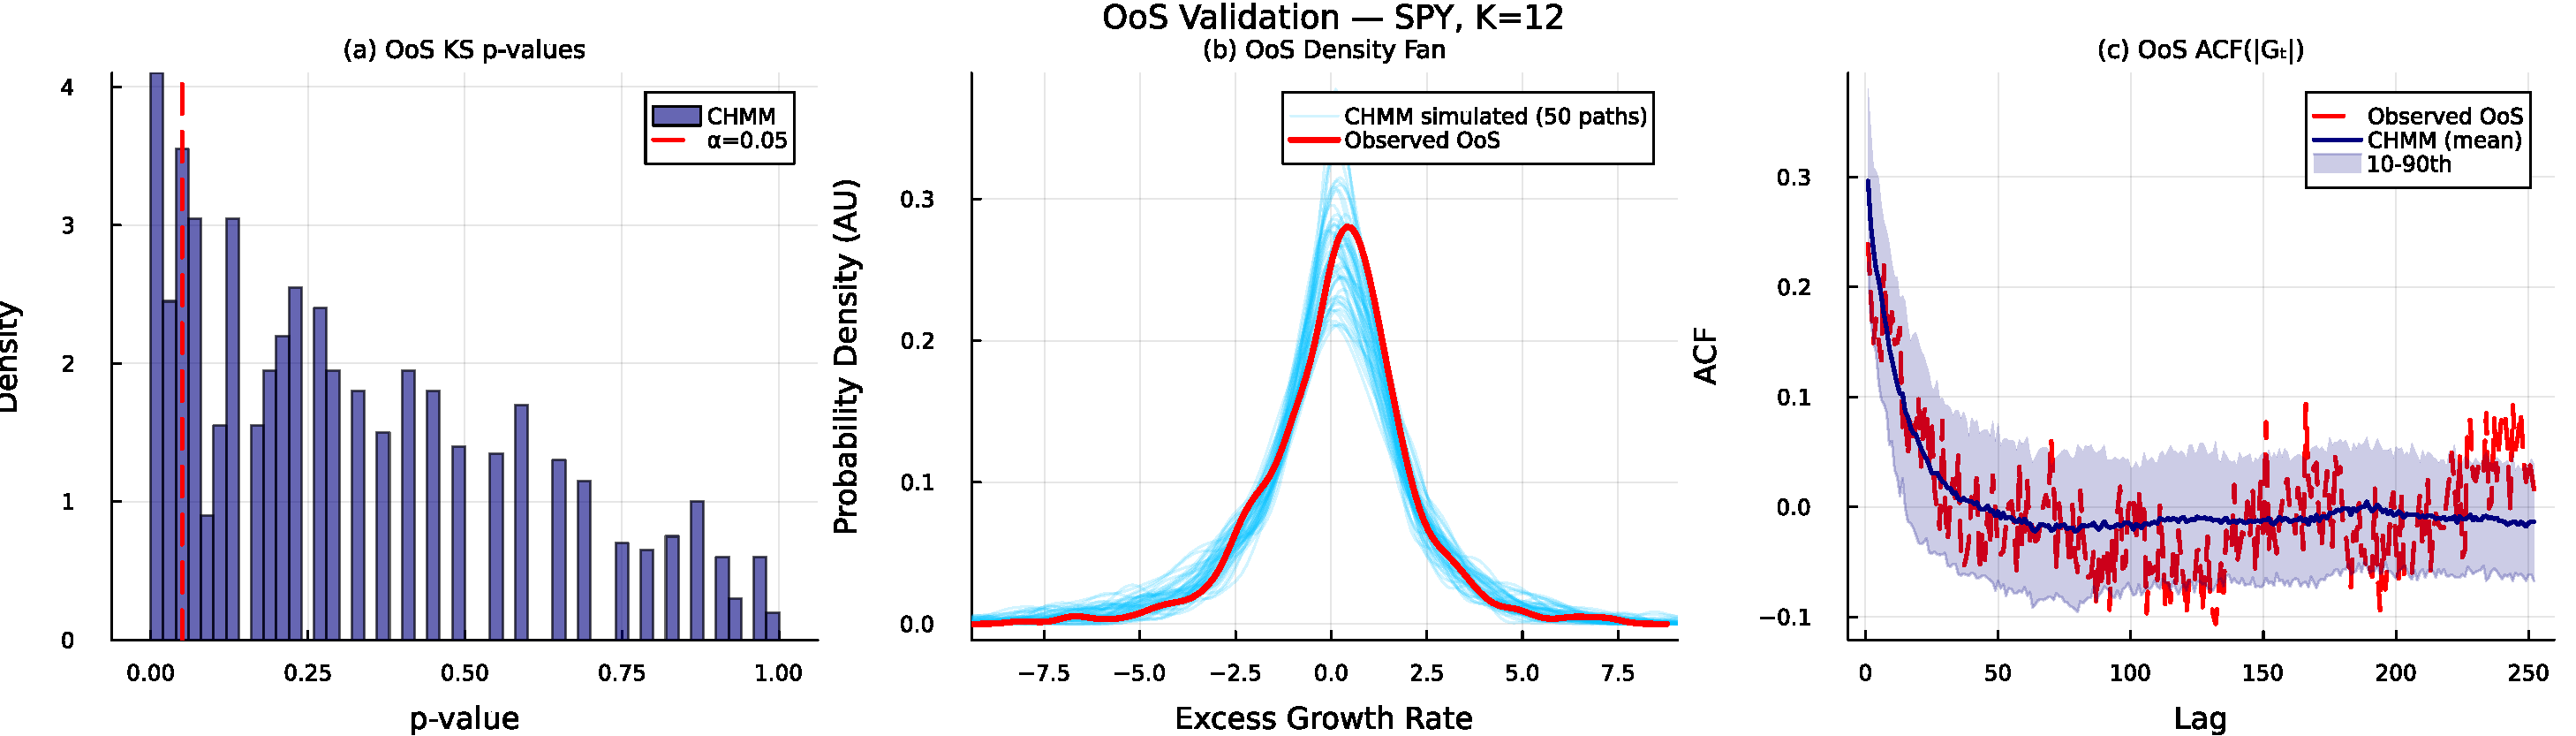
\includegraphics[width=\textwidth]{sections/figs/Fig-4-OoS-Validation-K12.pdf}
    \caption{$K = 12$}
\end{subfigure}
\hfill
\begin{subfigure}[b]{0.32\textwidth}
    
\includegraphics[width=\textwidth]{sections/figs/Fig-4-OoS-Validation-K15.pdf}
    \caption{$K = 15$}
\end{subfigure}
\hfill
\begin{subfigure}[b]{0.32\textwidth}
    
\includegraphics[width=\textwidth]{sections/figs/Fig-4-OoS-Validation-K21.pdf}
    \caption{$K = 21$}
\end{subfigure}
\caption{Out-of-sample CHMM validation panels at the non-selected state resolutions.}
\label{fig:k_sweep_panels_oos}
\end{figure}

\subsection{ACF Comparison Across State Resolutions}

Figure~\ref{fig:acf_all} shows the ACF of $|G_t|$ for the CHMM at $K = 3$, $K = 12$, and $K = 18$, compared to the observed ACF.
At all resolutions, the simulated ACF (shown as the median with 10th--90th percentile envelope across 1{,}000 paths) tracks the observed slow decay pattern.

\begin{figure}[H]
\centering
\begin{subfigure}[b]{0.32\textwidth}
    
\includegraphics[width=\textwidth]{sections/figs/Fig-ACF-Comparison-K3.pdf}
    \caption{$K = 3$}
\end{subfigure}
\hfill
\begin{subfigure}[b]{0.32\textwidth}
    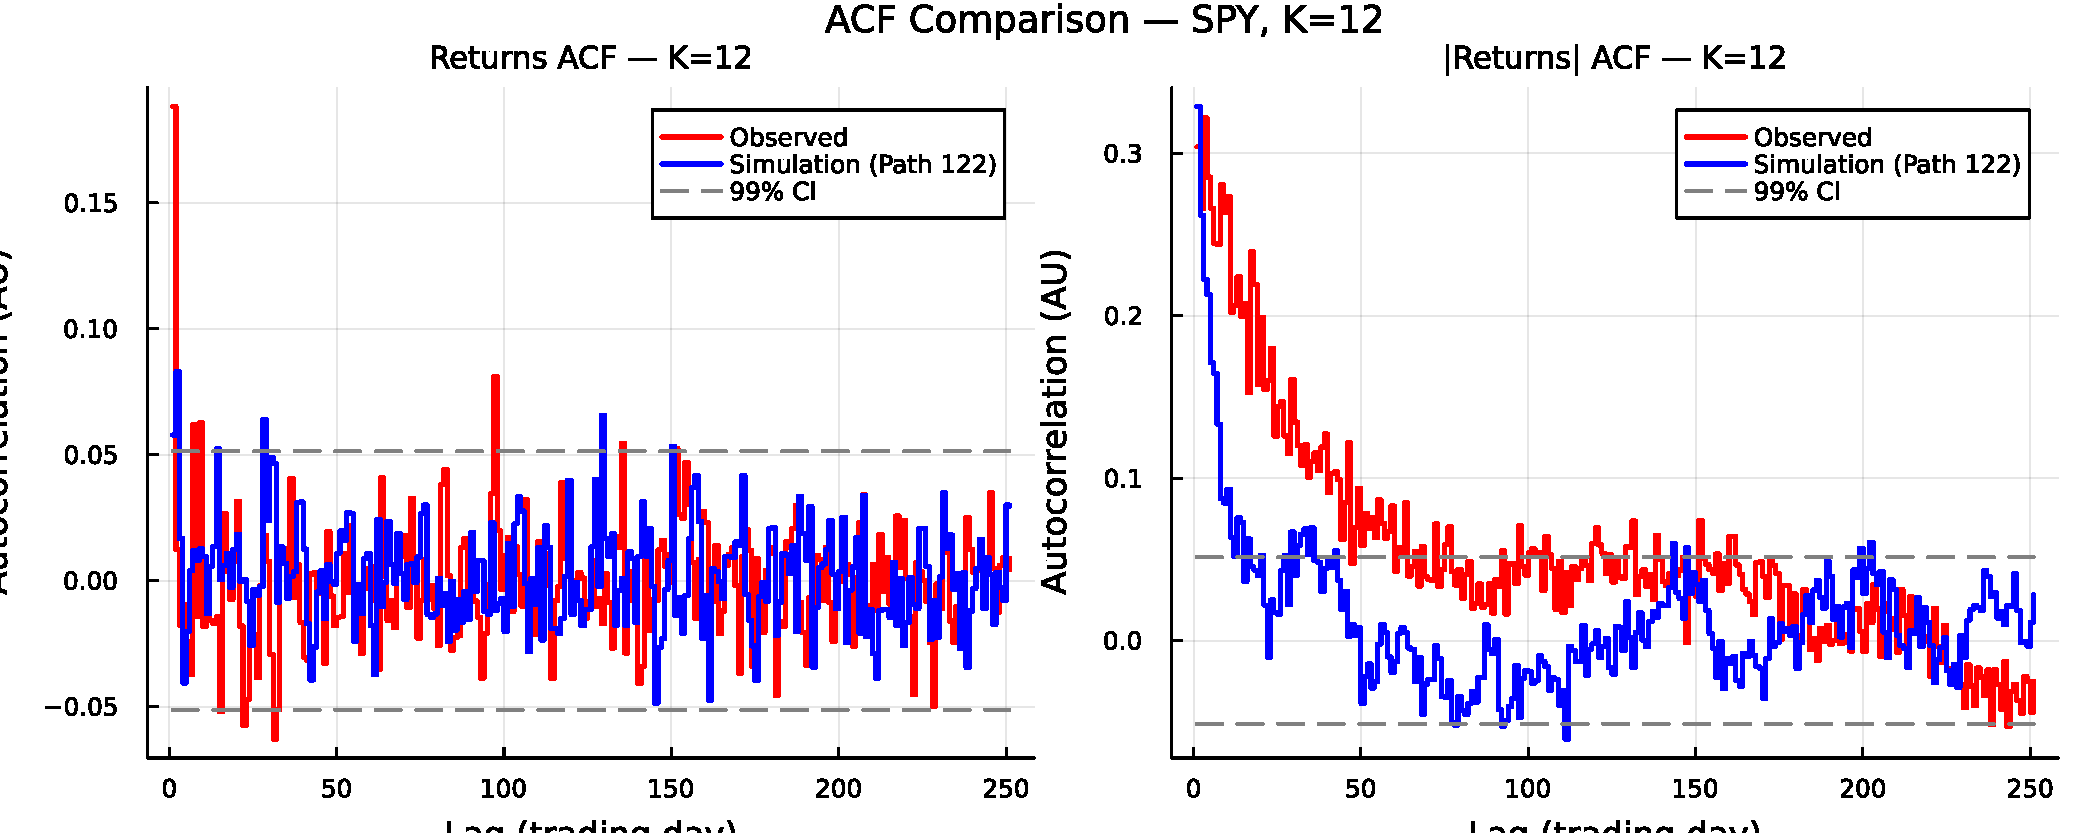
\includegraphics[width=\textwidth]{sections/figs/Fig-ACF-Comparison-K12.pdf}
    \caption{$K = 12$}
\end{subfigure}
\hfill
\begin{subfigure}[b]{0.32\textwidth}
    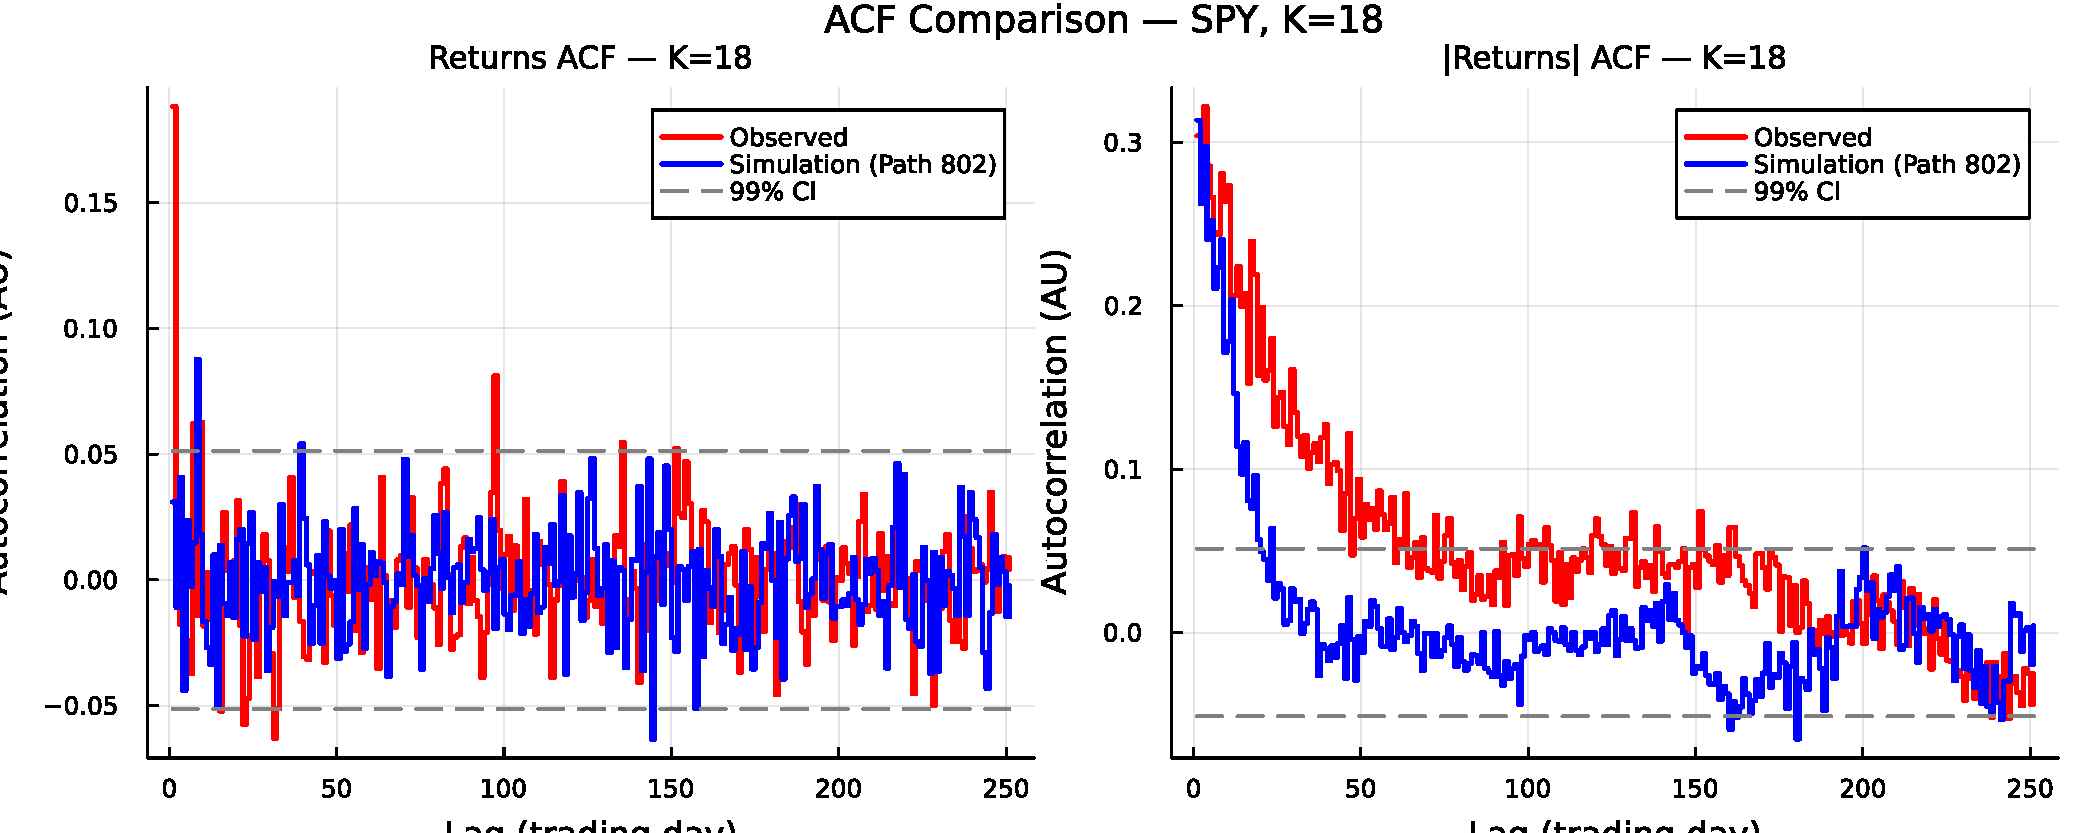
\includegraphics[width=\textwidth]{sections/figs/Fig-ACF-Comparison-K18.pdf}
    \caption{$K = 18$ (selected)}
\end{subfigure}
\caption{ACF of $|G_t|$ for the CHMM at $K = 3$, $K = 12$, and $K = 18$. The simulated 10th--90th percentile envelope (shaded) envelopes the observed ACF (red dashed), confirming that the CHMM reproduces volatility clustering without jump augmentation across the entire sweep.}
\label{fig:acf_all}
\end{figure}

\subsection{Example Simulated Trajectories}

Figure~\ref{fig:trajectories} shows example simulated return trajectories for $K = 6$ and $K = 18$, illustrating the qualitative dynamics produced by the CHMM.
Both trajectories exhibit the characteristic pattern of financial returns: extended periods of low volatility punctuated by clusters of large-magnitude events.

\begin{figure}[H]
\centering
\begin{subfigure}[b]{0.48\textwidth}
    
\includegraphics[width=\textwidth]{sections/figs/Fig-Trajectory-Example-K6.pdf}
    \caption{$K = 6$}
\end{subfigure}
\hfill
\begin{subfigure}[b]{0.48\textwidth}
    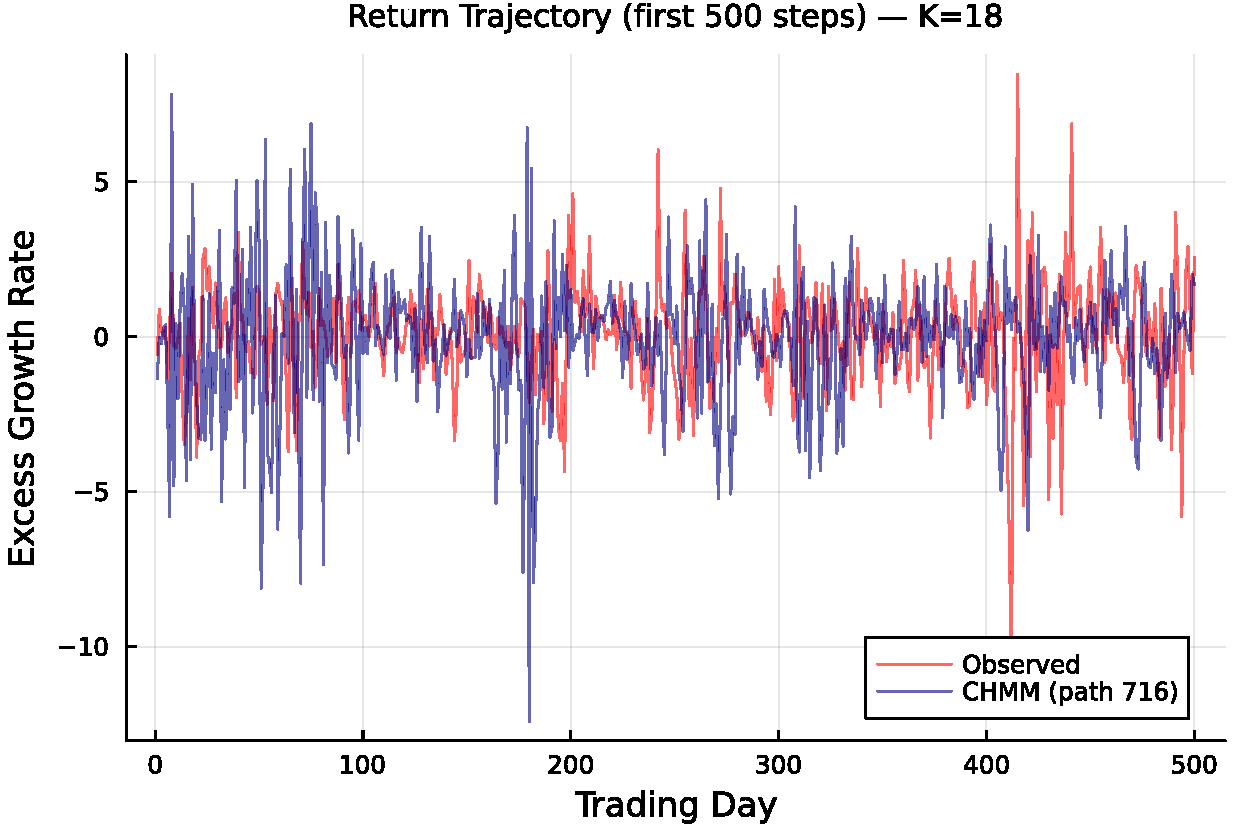
\includegraphics[width=\textwidth]{sections/figs/Fig-Trajectory-Example-K18.pdf}
    \caption{$K = 18$}
\end{subfigure}
\caption{Example simulated return trajectories. The alternation between calm (central states) and volatile (tail states) periods produces the volatility clustering characteristic of empirical financial returns.}
\label{fig:trajectories}
\end{figure}

\subsection{Multi-Emission Figures at $K = 18$}
\label{sec:multi_emission_figs}

This appendix reproduces the standard diagnostic suite (emission PDFs, transition matrix, stationary distribution, residence times, IS comparison, OoS validation, and convergence) for the two heavy-tailed emission families (CHMM-t and CHMM-L) at the selected state resolution $K = 18$.
The Gaussian counterparts are already shown as Figures~\ref{fig:model_internals},~\ref{fig:is_comparison},~\ref{fig:oos_validation},~\ref{fig:convergence_all},~\ref{fig:transition_all},~\ref{fig:stationary_all}, and~\ref{fig:residence_all} in the main text and above in this appendix.
The figures confirm that the shared forward--backward scaffold produces internally-similar regime structure across the three families: the near-diagonal transition band, the $K$-component dense emission cover, the longer central-state residence times, and the monotone log-likelihood convergence are features of the CHMM framework and not of the Gaussian component specifically.

\paragraph{Emission PDFs.}
Figure~\ref{fig:emissions_families} compares the learned $K = 18$ emissions for the three families.
The CHMM-t panel's per-state $\nu_k$ allocation is visible in the narrower modes of certain tail states; the CHMM-L panel's Laplace components have sharper peaks and slower exponential tail decay than the Gaussians.

\begin{figure}[H]
\centering
\begin{subfigure}[b]{0.32\textwidth}
    
\includegraphics[width=\textwidth]{sections/figs/Fig-Emission-PDFs-K18-N.pdf}
    \caption{CHMM-N (Gaussian)}
\end{subfigure}
\hfill
\begin{subfigure}[b]{0.32\textwidth}
    
\includegraphics[width=\textwidth]{sections/figs/Fig-Emission-PDFs-K18-t.pdf}
    \caption{CHMM-t (Student-t)}
\end{subfigure}
\hfill
\begin{subfigure}[b]{0.32\textwidth}
    
\includegraphics[width=\textwidth]{sections/figs/Fig-Emission-PDFs-K18-L.pdf}
    \caption{CHMM-L (Laplace)}
\end{subfigure}
\caption{Learned emission distributions at $K = 18$ across the three emission families, overlaid on the observed SPY return histogram. Heavier-tailed emission families (t, L) give individual components more tail mass, which is what closes the kurtosis gap of the Gaussian CHMM.}
\label{fig:emissions_families}
\end{figure}

\paragraph{Transition matrices.}
Figure~\ref{fig:transition_families} shows the $K = 18$ transition matrices learned by each family.
The near-diagonal band and the magnitude of self-transition probabilities are essentially unchanged across families, consistent with the ACF-MAE being stable across the family axis (Table~\ref{tab:sensitivity_multi}).

\begin{figure}[H]
\centering
\begin{subfigure}[b]{0.32\textwidth}
    
\includegraphics[width=\textwidth]{sections/figs/Fig-Transition-Matrix-K18-N.pdf}
    \caption{CHMM-N}
\end{subfigure}
\hfill
\begin{subfigure}[b]{0.32\textwidth}
    
\includegraphics[width=\textwidth]{sections/figs/Fig-Transition-Matrix-K18-t.pdf}
    \caption{CHMM-t}
\end{subfigure}
\hfill
\begin{subfigure}[b]{0.32\textwidth}
    
\includegraphics[width=\textwidth]{sections/figs/Fig-Transition-Matrix-K18-L.pdf}
    \caption{CHMM-L}
\end{subfigure}
\caption{Learned transition matrices at $K = 18$ in log$_{10}$ color scale. The diagonal-band structure is preserved across all three emission families.}
\label{fig:transition_families}
\end{figure}

\paragraph{Stationary distributions and residence times.}
Figure~\ref{fig:stationary_families} and Figure~\ref{fig:residence_families} compare the stationary distribution and natural residence times $\tau_k = 1/(1 - T_{kk})$ across families at $K = 18$.
The mass concentration at central states and the monotone decrease of $\tau_k$ toward the tails are features of the regime structure, not the emission family.

\begin{figure}[H]
\centering
\begin{subfigure}[b]{0.32\textwidth}
    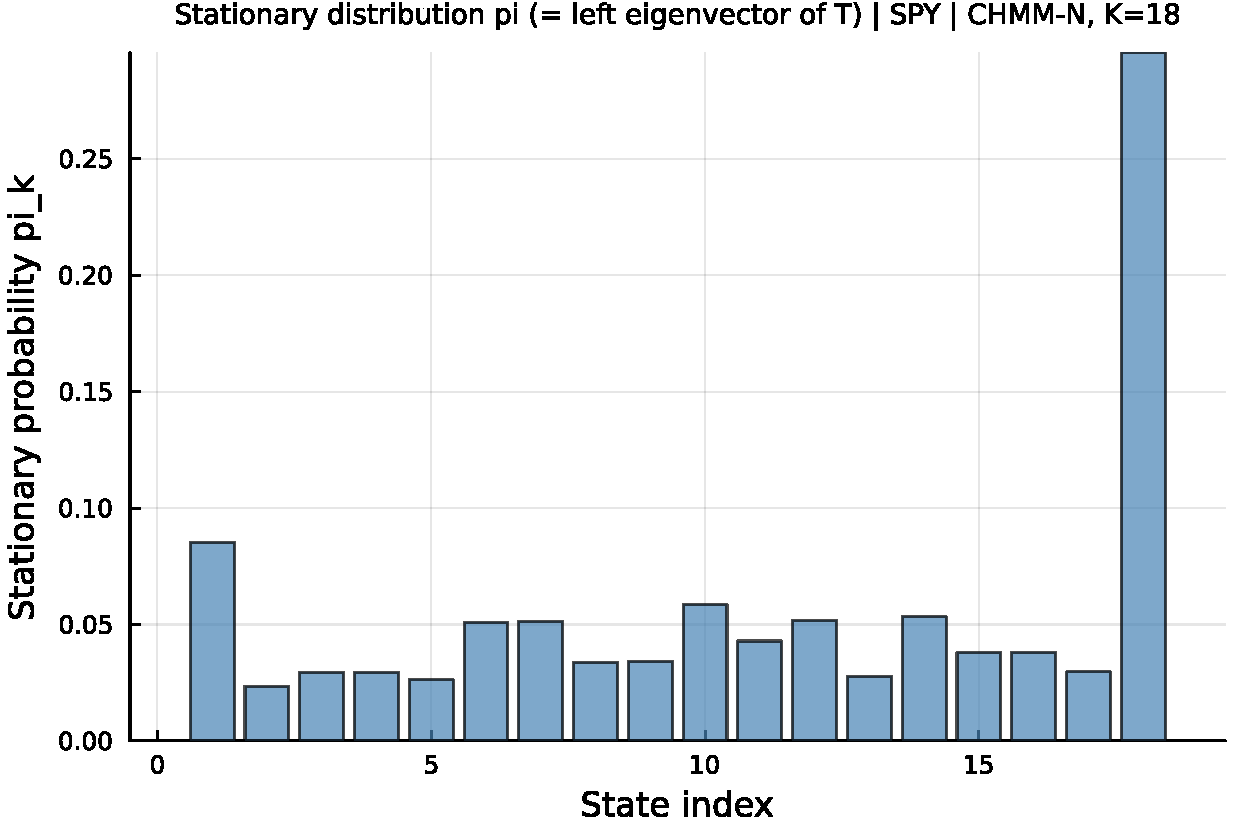
\includegraphics[width=\textwidth]{sections/figs/Fig-Stationary-Distribution-K18-N.pdf}
    \caption{CHMM-N}
\end{subfigure}
\hfill
\begin{subfigure}[b]{0.32\textwidth}
    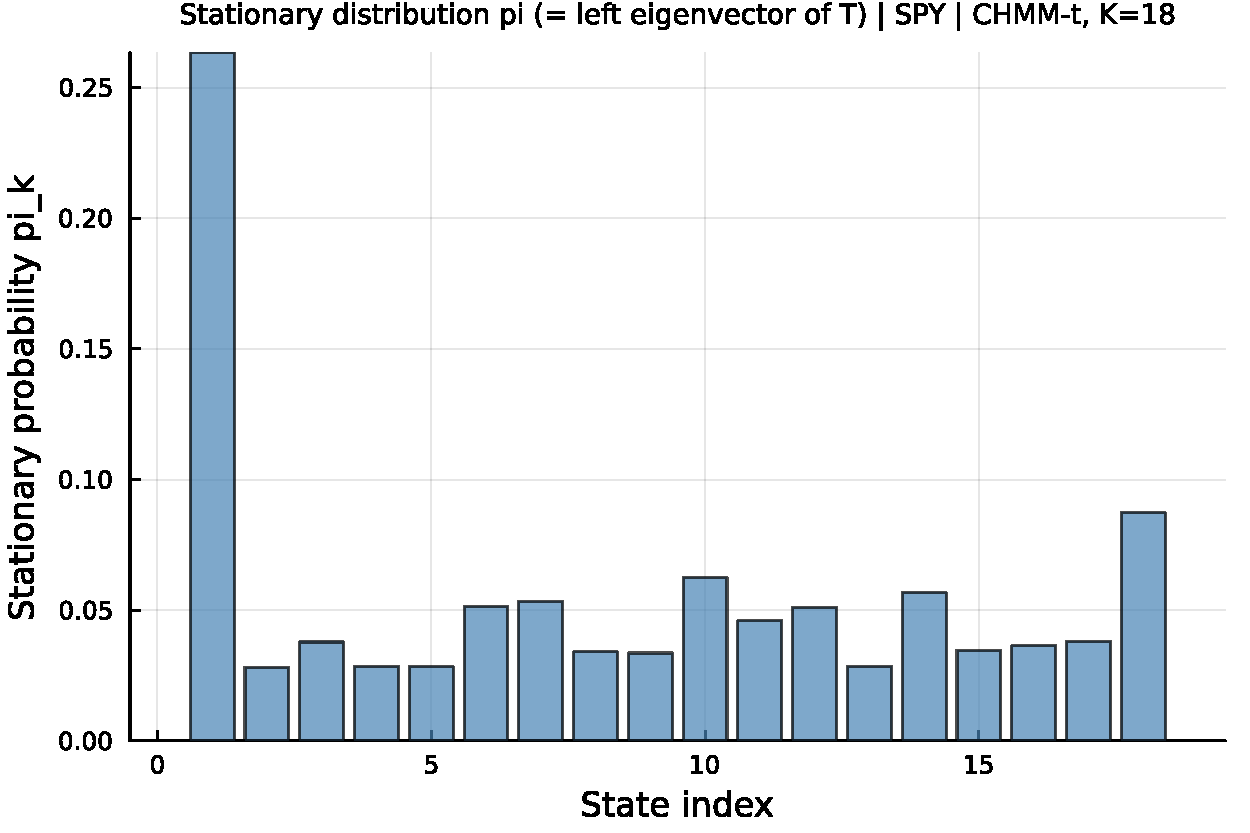
\includegraphics[width=\textwidth]{sections/figs/Fig-Stationary-Distribution-K18-t.pdf}
    \caption{CHMM-t}
\end{subfigure}
\hfill
\begin{subfigure}[b]{0.32\textwidth}
    
\includegraphics[width=\textwidth]{sections/figs/Fig-Stationary-Distribution-K18-L.pdf}
    \caption{CHMM-L}
\end{subfigure}
\caption{Stationary distributions $\bar{\boldsymbol{\pi}}$ at $K = 18$ across the three emission families.}
\label{fig:stationary_families}
\end{figure}

\begin{figure}[H]
\centering
\begin{subfigure}[b]{0.32\textwidth}
    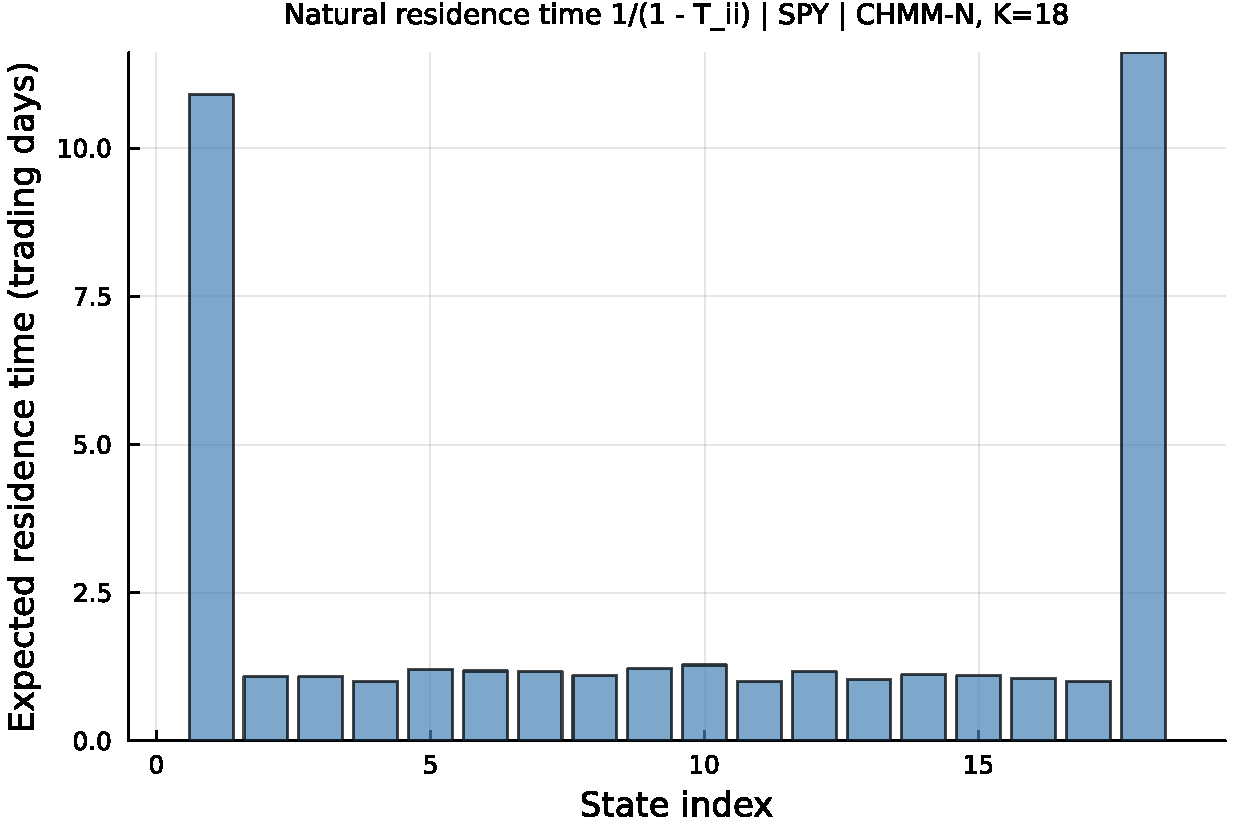
\includegraphics[width=\textwidth]{sections/figs/Fig-Residence-Times-K18-N.pdf}
    \caption{CHMM-N}
\end{subfigure}
\hfill
\begin{subfigure}[b]{0.32\textwidth}
    
\includegraphics[width=\textwidth]{sections/figs/Fig-Residence-Times-K18-t.pdf}
    \caption{CHMM-t}
\end{subfigure}
\hfill
\begin{subfigure}[b]{0.32\textwidth}
    
\includegraphics[width=\textwidth]{sections/figs/Fig-Residence-Times-K18-L.pdf}
    \caption{CHMM-L}
\end{subfigure}
\caption{Natural residence times $\tau_k = 1/(1 - T_{kk})$ at $K = 18$ across the three emission families.}
\label{fig:residence_families}
\end{figure}

\paragraph{In-sample comparison.}
Figure~\ref{fig:is_families} reproduces the three-panel in-sample comparison (density, ACF of $|G_t|$, tail Q-Q) at $K = 18$ for the two heavy-tailed families; the CHMM-N panel is Figure~\ref{fig:is_comparison} in the main text.

\begin{figure}[H]
\centering
\begin{subfigure}[b]{0.48\textwidth}
    
\includegraphics[width=\textwidth]{sections/figs/Fig-3-IS-Comparison-K18-t.pdf}
    \caption{CHMM-t}
\end{subfigure}
\hfill
\begin{subfigure}[b]{0.48\textwidth}
    
\includegraphics[width=\textwidth]{sections/figs/Fig-3-IS-Comparison-K18-L.pdf}
    \caption{CHMM-L}
\end{subfigure}
\caption{In-sample model comparison at $K = 18$ for the two heavy-tailed emission families. Each panel shows (a) marginal density with KS pass rate, (b) ACF of $|G_t|$, and (c) tail Q-Q plot. The CHMM-N counterpart is Figure~\ref{fig:is_comparison}.}
\label{fig:is_families}
\end{figure}

\paragraph{Out-of-sample validation.}
Figure~\ref{fig:oos_families} shows the OoS validation panels for CHMM-t and CHMM-L at $K = 18$.
The CHMM-t panel demonstrates the OoS kurtosis alignment noted in the main text (simulated 6.40 vs.\ observed 6.24), and the CHMM-L panel shows the tighter density fan produced by the heavier Laplace tails relative to the Gaussian.

\begin{figure}[H]
\centering
\begin{subfigure}[b]{0.48\textwidth}
    
\includegraphics[width=\textwidth]{sections/figs/Fig-4-OoS-Validation-K18-t.pdf}
    \caption{CHMM-t}
\end{subfigure}
\hfill
\begin{subfigure}[b]{0.48\textwidth}
    
\includegraphics[width=\textwidth]{sections/figs/Fig-4-OoS-Validation-K18-L.pdf}
    \caption{CHMM-L}
\end{subfigure}
\caption{Out-of-sample validation at $K = 18$ for the two heavy-tailed emission families. Each panel shows (a) KS $p$-values, (b) OoS density fan, and (c) OoS ACF of $|G_t|$. The CHMM-N counterpart is Figure~\ref{fig:oos_validation}.}
\label{fig:oos_families}
\end{figure}

\paragraph{Convergence.}
Figure~\ref{fig:convergence_families} shows the Baum-Welch / ECM / weighted-EM log-likelihood histories at $K = 18$ for all three families.
The CHMM-t and CHMM-L curves inherit the monotone increase of the classical EM guarantee; the CHMM-t curve has a slightly longer pre-plateau phase because each ECM sub-iteration refines $\nu_k$ with a golden-section search.

\begin{figure}[H]
\centering
\begin{subfigure}[b]{0.32\textwidth}
    
\includegraphics[width=\textwidth]{sections/figs/Fig-Convergence-K18-N.pdf}
    \caption{CHMM-N}
\end{subfigure}
\hfill
\begin{subfigure}[b]{0.32\textwidth}
    
\includegraphics[width=\textwidth]{sections/figs/Fig-Convergence-K18-t.pdf}
    \caption{CHMM-t}
\end{subfigure}
\hfill
\begin{subfigure}[b]{0.32\textwidth}
    
\includegraphics[width=\textwidth]{sections/figs/Fig-Convergence-K18-L.pdf}
    \caption{CHMM-L}
\end{subfigure}
\caption{Log-likelihood histories at $K = 18$ across the three emission families. All three curves are monotonically non-decreasing and plateau well before the $\texttt{max\_iter} = 60$ budget.}
\label{fig:convergence_families}
\end{figure}

\subsection{Cross-Asset Dependence Models: Derivations and Diagnostics}
\label{sec:cross_asset_supp}

This appendix provides the technical background for the SIM and copula constructions used in Section~\ref{sec:cross_asset} of the main text.

\paragraph{Sklar's theorem and the rank-reordering simulator.}
Sklar's theorem \cite{sklar1959fonctions, nelsen2006introduction} states that any $d$-dimensional joint CDF $H(g_1, \dots, g_d)$ with continuous marginals $F_1, \dots, F_d$ can be written as $H = C(F_1, \dots, F_d)$ for a unique copula $C$.
The rank-reordering simulator exploits this uniqueness.
If $\tilde{\mathbf{G}}$ is a matrix whose $j$-th column is an i.i.d.\ sample from $F_j$, and $\mathbf{U}$ is an independent sample from $C$, then reordering each column of $\tilde{\mathbf{G}}$ so that its ranks match $\mathbf{U}$'s produces a sample from $H$, up to discrete approximation error in the empirical ranks.
Crucially, reordering never creates new values: each column of the output is a permutation of the corresponding column of $\tilde{\mathbf{G}}$, so marginal distributions are preserved exactly \cite{iman1982distribution}.

\paragraph{Kendall's $\tau$ inversion.}
Given in-sample returns $\mathbf{R} \in \mathbb{R}^{T \times d}$, we estimate the pairwise Kendall's $\tau_{ij}$ from concordant/discordant pair counts and invert to the correlation scale via the analytic relationship $\rho_{ij} = \sin(\pi \tau_{ij} / 2)$, which holds exactly for the Gaussian copula family and is commonly used as a robust correlation estimator for the Student-t copula \cite{embrechts2002correlation, mcneil2015quantitative}.
The resulting matrix $\hat{\Sigma}$ is symmetric but not guaranteed positive semi-definite; we project to the nearest PSD matrix by clipping negative eigenvalues to $10^{-8}$ and rescaling the diagonal to unity.

\paragraph{Profile MLE for $\nu$.}
The Student-t copula log-density at a single pseudo-uniform observation $\mathbf{u} \in [0,1]^d$, with $x_j = t_\nu^{-1}(u_j)$ and $\mathbf{x} = (x_1, \dots, x_d)^\top$, is
\begin{align}
    \log c_t(\mathbf{u}; \Sigma, \nu)
    \;=\;&
    \log \Gamma\!\left(\tfrac{\nu+d}{2}\right)
    + (d-1)\,\log \Gamma\!\left(\tfrac{\nu}{2}\right)
    - d\,\log \Gamma\!\left(\tfrac{\nu+1}{2}\right)
    - \tfrac{1}{2} \log |\Sigma|
    \notag \\
    &\;
    - \tfrac{\nu+d}{2}\,\log\!\left(1 + \tfrac{\mathbf{x}^{\!\top} \Sigma^{-1} \mathbf{x}}{\nu}\right)
    + \sum_{j=1}^{d} \tfrac{\nu+1}{2}\,\log\!\left(1 + \tfrac{x_j^2}{\nu}\right).
    \label{eq:tcop_ll}
\end{align}
Summing over $t = 1, \dots, T$ pseudo-observations yields the profile log-likelihood as a function of $\nu$ with $\Sigma$ held fixed at the Kendall's-$\tau$ estimate.
We evaluate equation~\eqref{eq:tcop_ll} on the discrete grid $\nu \in \{2, 3, 4, 5, 6, 8, 10, 15, 20, 30\}$ and select $\hat{\nu}$ as the grid point with the largest total log-likelihood.
In Section~\ref{sec:cross_asset} the selected value was $\hat{\nu} = 6$ on the six-asset universe.

\paragraph{Sampling the copula.}
To sample $T$ rows from the $d$-dimensional Gaussian copula with correlation $\Sigma$, we (i) compute the Cholesky factor $\Sigma = L L^\top$, (ii) draw $Z \sim \mathcal{N}(0, I_d)$ i.i.d.\ and form $Y = L Z$, and (iii) return $U = \Phi(Y)$ componentwise.
For the Student-t copula with degrees of freedom $\nu$, we draw $W \sim \chi^2_\nu / \nu$ independent of $Y$ and form the multivariate-$t$ variate $X = Y / \sqrt{W}$, then return $U = t_\nu(X)$ componentwise.

\paragraph{SIM regression summary.}
Table~\ref{tab:sim_regression} reports the fitted SIM regression coefficients and goodness-of-fit statistics for the non-market assets in Section~\ref{sec:cross_asset}.
QQQ's high $R^2 = 0.841$ reflects that the Nasdaq-100 ETF is essentially a linear combination of large-cap technology names that also drive the S\&P~500 index, while JNJ's lower $R^2 = 0.225$ reflects the limited systematic exposure of low-beta healthcare stocks.
These factor loadings and residual magnitudes are what the SIM simulation in equation~\eqref{eq:sim_sim} re-injects at simulation time, and they explain the uneven per-asset KS pass rates reported in Table~\ref{tab:cross_asset_sim_copula}.

\begin{table}[H]
\centering
\caption{SIM regression $\hat{G}_{j,t} = \hat{\alpha}_j + \hat{\beta}_j G_{\text{SPY},t} + \hat{\eta}_{j,t}$ for the five non-market assets, fitted on the 2014--2024 in-sample window ($T = 2{,}766$). Coefficients $\hat{\alpha}, \hat{\beta}$ and $R^2$ are reported for the factor equation used in equation~\eqref{eq:sim_sim}.}
\label{tab:sim_regression}
\small
\begin{tabular}{l ccc}
\toprule
Ticker & $\hat{\alpha}$ & $\hat{\beta}$ & $R^2$ \\
\midrule
NVDA & $0.347$   & $1.749$ & $0.370$ \\
JNJ  & $-0.016$  & $0.539$ & $0.225$ \\
JPM  & $0.001$   & $1.204$ & $0.483$ \\
AAPL & $0.106$   & $1.194$ & $0.474$ \\
QQQ  & $0.041$   & $1.134$ & $0.841$ \\
\bottomrule
\end{tabular}
\end{table}

\subsection{VIX Results Detail}

The CHMM framework was applied to VIX daily log returns to test generalization beyond equity returns.
VIX returns exhibit positive skewness (reflecting asymmetric volatility spikes), pronounced mean reversion, and extreme excess kurtosis, properties that differ fundamentally from equity returns.

The CHMM captured these properties effectively: at higher state resolutions ($K \geq 9$), the model achieved IS KS pass rates above 99\%, demonstrating that the Gaussian mixture mechanism can approximate even the positively skewed, heavy-tailed marginal distribution of VIX returns.
The regime decomposition provided by the Viterbi algorithm aligned with known market events, assigning high-volatility states to crisis episodes and low-volatility states to calm market periods.

The VIX extension demonstrates that the CHMM framework is not limited to equity returns but applies more broadly to financial time series with regime-switching dynamics, including volatility measures used directly as synthetic-data targets.

\subsection{Algorithm Descriptions}
\label{sec:algorithms}

This section provides detailed pseudocode for the main algorithms used in this study.
Algorithm~\ref{alg:chmm_em} is the unified EM procedure shared across all three emission families.
It makes explicit the \emph{shared scaffold} (quantile-based initialization, log-space forward-backward, transition update) and the three \emph{family-specific branches} (Gaussian M-step for CHMM-N, ECM with one-dimensional golden-section $\nu$-search for CHMM-t, closed-form weighted-median + weighted-MAD for CHMM-L); the branch points are lines~\ref{line:init}, \ref{line:emit}, and \ref{line:mstep}.
Visualizing the three variants as a single algorithm with three M-step branches makes the architectural contribution of the paper --- one EM engine, three interchangeable emission families --- immediate from the pseudocode.
Algorithm~\ref{alg:viterbi} presents the Viterbi algorithm for decoding the most likely hidden state sequence.
Algorithm~\ref{alg:chmm_simulate} describes the CHMM simulation procedure for generating synthetic return paths.
Algorithm~\ref{alg:copula_sim} describes the cross-asset rank-reordering simulator for copula-based multi-asset synthesis.
Algorithm~\ref{alg:sim_build} details the SIM regression-and-resampling pipeline.

% ========================================================================================= %
% Algorithm 1: Baum-Welch (EM) for Continuous Gaussian HMM
% ========================================================================================= %
% Unified EM algorithm with family-specific M-step switch
% ========================================================================================= %
\begin{algorithm}[tp]
\caption{Unified EM algorithm for the CHMM family. Lines~\ref{line:init}, \ref{line:emit}, and \ref{line:mstep} branch on the emission family $F \in \{\mathcal{N}, t, L\}$; every other line is identical across families. CHMM-N and CHMM-L instantiate classical EM; CHMM-t instantiates an ECM sequence whose second CM step updates $\nu_k$ by a one-dimensional golden-section search on the per-state $Q$-function.}
\label{alg:chmm_em}
\small
\begin{algorithmic}[1]
\REQUIRE Observations $O_{1:T}$, number of states $K$, tolerance $\text{tol}$, $\texttt{max\_iter}$, emission family $F \in \{\mathcal{N}, t, L\}$, if $F = t$ bracket $(\nu_{\min}, \nu_{\max})$ and initial $\nu^{(0)}$.
\ENSURE Transition matrix $\mathbf{T}$, per-state emission parameters $\boldsymbol\theta_{1:K}$, initial distribution $\boldsymbol{\pi}$.

\STATE \textbf{Quantile-Based Initialization.}
\STATE Sort $O^{(\text{sort})} \leftarrow \text{sort}(O_{1:T})$ and partition into $K$ equal chunks $\{C_1,\ldots,C_K\}$.
\FOR{$k = 1$ to $K$} \label{line:init}
    \STATE \textbf{switch} $F$
    \STATE \quad $F = \mathcal{N}$: $\mu_k \leftarrow \text{mean}(C_k)$, \quad $\sigma_k \leftarrow \max(\text{std}(C_k), 10^{-6})$.
    \STATE \quad $F = t$: $\mu_k \leftarrow \text{mean}(C_k)$, \quad $\sigma_k \leftarrow \max(\text{std}(C_k), 10^{-6})$, \quad $\nu_k \leftarrow \nu^{(0)}$.
    \STATE \quad $F = L$: $\mu_k \leftarrow \text{median}(C_k)$, \quad $b_k \leftarrow \max(\text{mean}(|C_k - \mu_k|), 10^{-6})$.
\ENDFOR
\STATE $T_{ij} \leftarrow 1/K$; \quad $\pi_k \leftarrow 1/K$; \quad $\mathcal{L}_{\text{prev}} \leftarrow -\infty$.

\STATE \textbf{EM Loop.}
\FOR{$n = 1$ to $\texttt{max\_iter}$}

    \STATE \textbf{E-Step --- per-family emission log-likelihood.} \label{line:emit}
    \STATE \textbf{switch} $F$
    \STATE \quad $F = \mathcal{N}$: $\log B_{t,k} \leftarrow \log \mathcal{N}(O_t \mid \mu_k, \sigma_k^2)$.
    \STATE \quad $F = t$: $\log B_{t,k} \leftarrow \log t_{\nu_k}(O_t; \mu_k, \sigma_k)$.
    \STATE \quad $F = L$: $\log B_{t,k} \leftarrow -\log(2 b_k) - |O_t - \mu_k|/b_k$.

    \STATE \textbf{E-Step --- shared log-space forward-backward.}
    \STATE $\log \alpha_1(k) \leftarrow \log \pi_k + \log B_{1,k}$.
    \FOR{$t = 2$ to $T$, $j = 1$ to $K$}
        \STATE $\log \alpha_t(j) \leftarrow \underset{i}{\text{logsumexp}}\!\left(\log \alpha_{t-1}(i) + \log T_{ij}\right) + \log B_{t,j}$.
    \ENDFOR
    \STATE $\log \beta_T(k) \leftarrow 0$.
    \FOR{$t = T-1$ down to $1$, $i = 1$ to $K$}
        \STATE $\log \beta_t(i) \leftarrow \underset{j}{\text{logsumexp}}\!\left(\log T_{ij} + \log B_{t+1,j} + \log \beta_{t+1}(j)\right)$.
    \ENDFOR
    \STATE Compute $\gamma_t(k)$ and $\xi_t(i,j)$ from equation~\eqref{eq:gamma_xi}.

    \STATE \textbf{Shared transition update.} $T_{ij} \leftarrow \sum_t \xi_t(i,j) \;/\; \sum_t \gamma_t(i)$; $\pi_k \leftarrow \gamma_1(k)$.

    \STATE \textbf{M-Step --- per-family emission update.} \label{line:mstep}
    \STATE \textbf{switch} $F$
    \STATE \quad $F = \mathcal{N}$ \COMMENT{classical Baum-Welch \citep{baum1970maximization}.}
    \STATE \qquad $\mu_k \leftarrow \sum_t \gamma_t(k)\, O_t / \sum_t \gamma_t(k)$.
    \STATE \qquad $\sigma_k \leftarrow \max\!\left(\sqrt{\sum_t \gamma_t(k) (O_t - \mu_k)^2 / \sum_t \gamma_t(k)},\; 10^{-6}\right)$.
    \STATE \quad $F = t$ \COMMENT{ECM of \citet{peel2000robust, liu1995ml}; closed-form $(\mu_k, \sigma_k)$ given $\nu_k$, then 1D search on $\nu_k$.}
    \STATE \qquad $u_{t,k} \leftarrow (\nu_k + 1) / (\nu_k + ((O_t - \mu_k)/\sigma_k)^2)$ for all $t, k$.
    \STATE \qquad $\mu_k \leftarrow \sum_t \gamma_t(k)\, u_{t,k}\, O_t / \sum_t \gamma_t(k)\, u_{t,k}$.
    \STATE \qquad $\sigma_k \leftarrow \max\!\left(\sqrt{\sum_t \gamma_t(k)\, u_{t,k}\,(O_t - \mu_k)^2 / \sum_t \gamma_t(k)},\; 10^{-6}\right)$.
    \STATE \qquad $\nu_k \leftarrow \arg\max_{\nu \in [\nu_{\min}, \nu_{\max}]} \sum_t \gamma_t(k)\, \log t_\nu(O_t; \mu_k, \sigma_k)$ \COMMENT{40-iter golden-section search.}
    \STATE \quad $F = L$ \COMMENT{closed-form weighted Laplace MLE.}
    \STATE \qquad $\mu_k \leftarrow \text{WeightedMedian}(O_{1:T},\, \gamma_{1:T}(k))$ \COMMENT{cumulative-weight bracketing with interpolation at the $W_k/2$ crossing.}
    \STATE \qquad $b_k \leftarrow \max\!\left(\sum_t \gamma_t(k)\, |O_t - \mu_k| / \sum_t \gamma_t(k),\; 10^{-6}\right)$.

    \STATE \textbf{Convergence check.} $\mathcal{L}^{(n)} \leftarrow \underset{k}{\text{logsumexp}}(\log \alpha_T(k))$.
    \IF{$|\mathcal{L}^{(n)} - \mathcal{L}_{\text{prev}}| < \text{tol}$} \STATE \textbf{break} \ENDIF
    \STATE $\mathcal{L}_{\text{prev}} \leftarrow \mathcal{L}^{(n)}$.
\ENDFOR

\RETURN $\mathbf{T}, \boldsymbol\theta_{1:K}, \boldsymbol{\pi}$ \COMMENT{$\boldsymbol\theta_k = (\mu_k, \sigma_k)$ for $F = \mathcal{N}$; $(\mu_k, \sigma_k, \nu_k)$ for $F = t$; $(\mu_k, b_k)$ for $F = L$.}
\end{algorithmic}
\end{algorithm}

% Backward-compatibility labels: any older cross-reference to the separate algorithms now points at the unified block.
\newcommand{\algbaumwelch}{\ref{alg:chmm_em}}
\newcommand{\algecmstudentt}{\ref{alg:chmm_em}}
\newcommand{\algemlaplace}{\ref{alg:chmm_em}}

% ========================================================================================= %
% Algorithm 2: Viterbi Decoding
% ========================================================================================= %
\begin{algorithm}[tp]
\caption{Viterbi decoding for the most likely hidden state sequence}
\label{alg:viterbi}
\small
\begin{algorithmic}[1]
\REQUIRE Observations $O_{1:T}$, Trained CHMM $\mathcal{M} = (\mathbf{T}, \{\mu_k, \sigma_k\}, \boldsymbol{\pi})$
\ENSURE Most probable state sequence $S_{1:T}^*$

\FOR{$k = 1$ to $K$}
    \STATE $\log \delta_1(k) \leftarrow \log(1/K) + \log \mathcal{N}(O_1 \mid \mu_k, \sigma_k^2)$.
\ENDFOR

\FOR{$t = 2$ to $T$}
    \FOR{$j = 1$ to $K$}
        \STATE $\text{vals}(i) \leftarrow \log \delta_{t-1}(i) + \log T_{ij}$ for all $i$.
        \STATE $\log \delta_t(j) \leftarrow \max_i \text{vals}(i) + \log \mathcal{N}(O_t \mid \mu_j, \sigma_j^2)$.
        \STATE $\psi_t(j) \leftarrow \arg\max_i \text{vals}(i)$.
    \ENDFOR
\ENDFOR

\STATE $S_T^* \leftarrow \arg\max_k \log \delta_T(k)$.
\FOR{$t = T-1$ down to $1$}
    \STATE $S_t^* \leftarrow \psi_{t+1}(S_{t+1}^*)$.
\ENDFOR

\RETURN $S_{1:T}^*$
\end{algorithmic}
\end{algorithm}

% ========================================================================================= %
% Algorithm 3: CHMM Simulation
% ========================================================================================= %
\begin{algorithm}[tp]
\caption{CHMM simulation of synthetic excess growth rate paths}
\label{alg:chmm_simulate}
\small
\begin{algorithmic}[1]
\REQUIRE Trained CHMM $\mathcal{M} = (\mathbf{T}, \{\mu_k, \sigma_k\}, \boldsymbol{\pi})$, Number of steps $M$, Number of paths $P$
\ENSURE Simulated return paths $\{\hat{G}^{(p)}_{1:M}\}_{p=1}^{P}$

\FOR{$p = 1$ to $P$}
    \STATE Sample initial state $S_1 \sim \text{Categorical}(\boldsymbol{\pi})$.
    \FOR{$t = 1$ to $M$}
        \STATE Emit observation $\hat{G}_t^{(p)} \sim \mathcal{N}(\mu_{S_t}, \sigma_{S_t}^2)$.
        \IF{$t < M$}
            \STATE Transition to next state $S_{t+1} \sim \text{Categorical}(\mathbf{T}_{S_t, \cdot})$.
        \ENDIF
    \ENDFOR
\ENDFOR

\RETURN $\{\hat{G}^{(p)}_{1:M}\}_{p=1}^{P}$
\end{algorithmic}
\end{algorithm}

% ========================================================================================= %
% Algorithm 4: Cross-Asset Copula Rank Reordering Simulation
% ========================================================================================= %
\begin{algorithm}[tp]
\caption{Cross-asset copula simulation via rank reordering}
\label{alg:copula_sim}
\small
\begin{algorithmic}[1]
\REQUIRE Fitted per-asset CHMMs $\{\mathcal{M}_j\}_{j=1}^d$, correlation matrix $\Sigma$ (PSD, unit diagonal), copula family $\mathcal{C} \in \{\text{Gaussian}, t_\nu\}$, path length $T$, number of paths $P$
\ENSURE Cross-asset path tensor $\{\hat{G}^{(p)}_{j,t}\}$ of shape $T \times d \times P$

\FOR{$p = 1$ to $P$}

    \STATE Draw copula sample $\mathbf{U}^{(p)} \in [0,1]^{T \times d}$ from $\mathcal{C}(\Sigma)$:
    \STATE \quad $L \leftarrow \text{Cholesky}(\Sigma)$, \; $Z \in \mathbb{R}^{T \times d} \sim \mathcal{N}(0, I_d)$ i.i.d.
    \STATE \quad $Y \leftarrow Z L^\top$
    \IF{$\mathcal{C} = $ Gaussian}
        \STATE \quad $\mathbf{U}^{(p)} \leftarrow \Phi(Y)$ componentwise
    \ELSE
        \STATE \quad Draw $W \sim \chi^2_\nu / \nu$ i.i.d. for $t = 1, \dots, T$; \; $X_{t,\cdot} \leftarrow Y_{t,\cdot} / \sqrt{W_t}$
        \STATE \quad $\mathbf{U}^{(p)} \leftarrow t_\nu(X)$ componentwise
    \ENDIF

    \FOR{$j = 1$ to $d$}
        \STATE Simulate $\tilde{g}_{j,1:T}^{(p)}$ from $\mathcal{M}_j$ via Algorithm~\ref{alg:chmm_simulate}.
        \STATE Compute order statistics $\tilde{g}_{j,(1)}^{(p)} \leq \cdots \leq \tilde{g}_{j,(T)}^{(p)}$.
        \STATE Compute ranks $r_{j,t}^{(p)} \leftarrow \text{rank}(U_{j,t}^{(p)})$ for $t = 1, \dots, T$.
        \STATE $\hat{G}_{j,t}^{(p)} \leftarrow \tilde{g}_{j,(r_{j,t}^{(p)})}^{(p)}$ for $t = 1, \dots, T$.
    \ENDFOR
\ENDFOR

\RETURN $\{\hat{G}^{(p)}_{j,t}\}$
\end{algorithmic}
\end{algorithm}

% ========================================================================================= %
% Algorithm 5: SIM fit and simulate
% ========================================================================================= %
\begin{algorithm}[tp]
\caption{Single Index Model (SIM) construction and simulation}
\label{alg:sim_build}
\small
\begin{algorithmic}[1]
\REQUIRE In-sample return matrix $\mathbf{R} \in \mathbb{R}^{T \times d}$, market-column index $m$, market CHMM $\mathcal{M}_m$, path length $T$, number of paths $P$
\ENSURE Cross-asset path tensor $\{\hat{G}^{(p)}_{j,t}\}$ of shape $T \times d \times P$

\STATE \textbf{OLS fit.} For $j \neq m$:
\STATE \quad $\hat{\beta}_j \leftarrow \text{Cov}(\mathbf{R}_{:,j}, \mathbf{R}_{:,m}) / \text{Var}(\mathbf{R}_{:,m})$
\STATE \quad $\hat{\alpha}_j \leftarrow \overline{\mathbf{R}_{:,j}} - \hat{\beta}_j \overline{\mathbf{R}_{:,m}}$
\STATE \quad $\hat{\eta}_{j,t} \leftarrow R_{t,j} - \hat{\alpha}_j - \hat{\beta}_j R_{t,m}$, \; $R^2_j \leftarrow 1 - \sum_t \hat{\eta}_{j,t}^2 / \sum_t (R_{t,j} - \overline{\mathbf{R}_{:,j}})^2$

\FOR{$p = 1$ to $P$}
    \STATE Simulate market path $G_{m,1:T}^{(p)}$ from $\mathcal{M}_m$ via Algorithm~\ref{alg:chmm_simulate}.
    \STATE $\hat{G}_{m,t}^{(p)} \leftarrow G_{m,t}^{(p)}$.
    \FOR{$j \neq m$}
        \STATE Draw residual indices $\{\iota_t\}_{t=1}^T \sim \text{Uniform}(\{1, \dots, T\})$.
        \STATE $\hat{G}_{j,t}^{(p)} \leftarrow \hat{\alpha}_j + \hat{\beta}_j G_{m,t}^{(p)} + \hat{\eta}_{j,\iota_t}$.
    \ENDFOR
\ENDFOR

\RETURN $\{\hat{G}^{(p)}_{j,t}\}$
\end{algorithmic}
\end{algorithm}


% =========================================================================== %
% v7 revision supplemental
% =========================================================================== %

\subsection{CHMM-t Degrees-of-Freedom Diagnostics}
\label{sec:nu_diagnostics}

This appendix backs the discussion in Section~\ref{sec:discussion} of the CHMM-t in-sample kurtosis overshoot.
Figure~\ref{fig:nu_hist} plots the per-state $\nu_k$ histogram for the $K = 18$ CHMM-t fit on SPY IS (seed = $20260420$).
Twelve of the eighteen states rest at the upper ECM bracket ($\nu_k = 50$), and only two states lie near the lower bracket ($\nu_2 = 2.35$, $\nu_4 = 2.82$).
The simulated in-sample mixture kurtosis of $12.60$ is driven by the posterior mass routed to those two very heavy-tailed states, not by a systemic collapse to the lower bracket.

\begin{figure}[h]
\centering
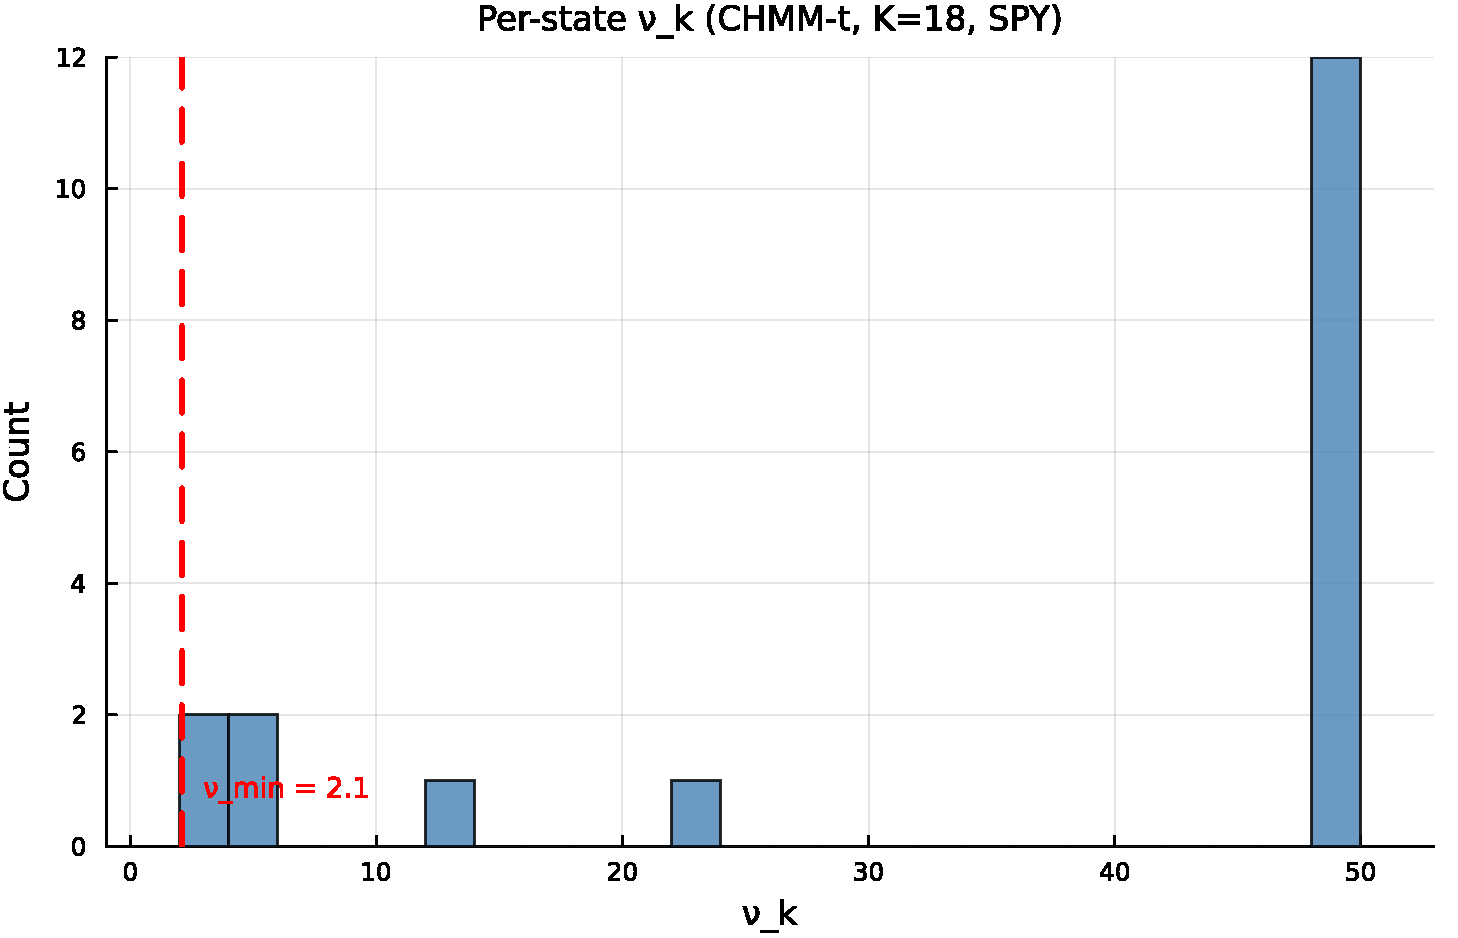
\includegraphics[width=0.75\textwidth]{sections/figs/Fig-v7-nu-Histogram.pdf}
\caption{Per-state degrees-of-freedom $\nu_k$ for the CHMM-t fit at $K = 18$ on SPY IS. The dashed red line marks the lower ECM bracket $\nu_{\min} = 2.1$. Only two states ($\nu_2 = 2.35$, $\nu_4 = 2.82$) sit near the lower bracket; the median $\nu_k$ is at the upper bracket.}
\label{fig:nu_hist}
\end{figure}

Table~\ref{tab:nu_bracket} reports the seven-metric panel for CHMM-t fits whose ECM bracket lower bound is lifted from $\nu_{\min} = 2.1$ through $\{2.5, 3.0, 4.0\}$, plus the Gaussian limit ($\nu = \infty$, equivalent to CHMM-N).
Lifting the bracket does not reduce the in-sample kurtosis overshoot: the simulated kurtosis moves within the $12.5$--$14.0$ band across bracket floors and only collapses to $5.05$ in the full Gaussian limit.
The overshoot is therefore a feature of the Student-t emission family at $K = 18$ and not a lower-bracket artefact.

\begin{table}[h]
\centering
\small
\caption{CHMM-t $\nu_{\min}$ bracket sensitivity at $K = 18$ on SPY (seed = 20260420, 1000 paths).}
\label{tab:nu_bracket}
\begin{tabular}{l cc cc cc c c c}
\toprule
$\nu_{\min}$ & KS IS & AD IS & KS OoS & AD OoS & Kurt IS & Kurt OoS & ACF-MAE & $W_1$ & $H$ \\
\midrule
$2.1$     & 94.2 & 89.4 & 95.5 & 90.1 & 12.50 & 6.95 & 0.0538 & 0.094 & 0.0725 \\
$2.5$     & 95.7 & 91.9 & 94.5 & 89.7 & 13.94 & 5.97 & 0.0536 & 0.094 & 0.0725 \\
$3.0$     & 95.6 & 91.4 & 93.8 & 89.7 & 14.04 & 6.25 & 0.0537 & 0.092 & 0.0725 \\
$4.0$     & 95.8 & 92.2 & 94.8 & 90.1 & 13.71 & 6.72 & 0.0535 & 0.092 & 0.0721 \\
$\infty$ (Gauss) & 96.6 & 88.6 & 94.3 & 87.9 & 5.05  & 3.47 & 0.0503 & 0.101 & 0.0770 \\
\midrule
\textit{Observed} & -- & -- & -- & -- & 7.71 & 6.24 & -- & -- & -- \\
\bottomrule
\end{tabular}
\end{table}

\subsection{Ryd\'en K = 2 Replication}
\label{sec:ryden_replication}

Table~\ref{tab:ryden_init} reports the direct replication of Ryd\'en et al.'s 1998 $K = 2$ setting on SPY IS under both initialization strategies, as discussed in Section~\ref{sec:discussion}.
The quantile-based initialization used in the main body is row 1; five independent random-seed initializations are rows 2--6.
Random init here draws per-state $(\mu_k, \sigma_k)$ from a moderate perturbation of the sample moments, which is representative of the random-init practice common in the 1990s HMM literature.

\begin{table}[h]
\centering
\small
\caption{Ryd\'en replication: $K = 2$ CHMM-N on SPY IS under quantile vs random initialization (seed sub-index varies the random init).}
\label{tab:ryden_init}
\begin{tabular}{l c c c c c}
\toprule
Init & KS IS (\%) & AD IS (\%) & ACF-MAE & Kurt IS & KS OoS (\%) \\
\midrule
Quantile (main body) & 71.8 & 68.3 & 0.0499 & 2.58 & 93.3 \\
Random seed = 1      & 72.2 & 70.0 & 0.0499 & 2.61 & 93.5 \\
Random seed = 7      & 67.9 & 65.7 & 0.0497 & 2.58 & 93.8 \\
Random seed = 42     & 69.9 & 66.0 & 0.0501 & 2.57 & 91.9 \\
Random seed = 100    & 69.1 & 67.4 & 0.0503 & 2.60 & 93.7 \\
Random seed = 2024   & 68.5 & 65.6 & 0.0498 & 2.58 & 94.0 \\
\bottomrule
\end{tabular}
\end{table}

The key observation is that ACF-MAE is essentially constant at $\approx 0.050$ across all six rows, matching the $K = 18$ CHMM-N of the main body.
In-sample KS pass rate remains below the $K = 18$ operating point (67.9--72.2\%) because two Gaussian components cannot tile the full multi-regime return distribution.
The combination confirms that the Ryd\'en low-$K$ limitation is a distributional (not temporal) artefact: the ACF is already well reproduced at $K = 2$, and it is distributional fidelity that drives the preference for $K = 18$.

\subsection{OoS KS Test-Power Calibration}
\label{sec:ks_power}

Table~\ref{tab:ks_power} reports the two-sample KS test-power calibration used to anchor the OoS KS pass rates of Section~\ref{sec:oos}.
For each of $1{,}000$ Monte Carlo replications (seed = 20260420), a simulated series of length $T_{\text{OoS}} = 219$ is drawn from each of three reference generators and tested against the observed OoS series using the same $\alpha = 0.05$ threshold as the main-body pass-rate metric.

\begin{table}[h]
\centering
\small
\caption{OoS KS pass-rate calibration (1000 replications, seed = 20260420).}
\label{tab:ks_power}
\begin{tabular}{l c}
\toprule
Reference generator & Pass rate (\%) \\
\midrule
I.i.d.\ resamples of $R_{\text{OoS}}$ at length $T_{\text{OoS}} = 219$ (known-correct ceiling) & 100.0 \\
I.i.d.\ resamples of $R_{\text{IS}}$ at length $T_{\text{OoS}} = 219$ (nearly correct)          & 98.4 \\
Gaussian$(\hat\mu_{\text{IS}}, \hat\sigma_{\text{IS}})$ at length $T_{\text{IS}}$ (negative control) & 0.0 \\
\bottomrule
\end{tabular}
\end{table}

The $98.4\%$ rate is the practical ceiling for the CHMM OoS KS pass rates reported in Section~\ref{sec:oos} ($93$--$96\%$); the $0\%$ rate on the Gaussian misspecified generator confirms that the KS test retains ample power at IS length to reject clearly wrong generators.

\subsection{Walk-Forward Rolling-Window Re-Estimation}
\label{sec:walk_forward}

Table~\ref{tab:walk_forward} reports the quarterly walk-forward re-estimation results referenced in Section~\ref{sec:cross_asset_univariate}.
The walk-forward protocol refits the CHMM-N every $63$ trading days (one quarter), feeding the realized returns of the prior quarter into the training set before each refit.
On both defensive tickers the rolling protocol recovers $1$--$2$ percentage points of OoS KS and AD relative to the fixed-IS baseline, consistent with the stationarity explanation for the OoS gap while leaving a residual term that a richer time-varying extension would be needed to close.

\begin{table}[h]
\centering
\small
\caption{Walk-forward (quarterly CHMM-N refit) vs fixed-IS CHMM-N on the two defensives (JNJ, JPM) at $K = 18$, 1000 paths (seed = 20260420).}
\label{tab:walk_forward}
\begin{tabular}{l cc cc cc c c c}
\toprule
Mode & KS IS & AD IS & KS OoS & AD OoS & Kurt IS & Kurt OoS & ACF-MAE & $W_1$ & $H$ \\
\midrule
JNJ fixed-IS      & 99.7 & 99.4 & 70.2 & 61.5 & 5.68 & 4.63 & 0.0319 & 0.083 & 0.0759 \\
JNJ walk-forward  & 99.7 & 99.4 & 71.0 & 62.9 & 5.68 & 4.51 & 0.0319 & 0.083 & 0.0759 \\
JPM fixed-IS      & 98.7 & 96.2 & 74.9 & 76.5 & 7.97 & 5.08 & 0.0431 & 0.154 & 0.0839 \\
JPM walk-forward  & 98.7 & 96.2 & 76.8 & 78.1 & 7.97 & 4.92 & 0.0431 & 0.154 & 0.0839 \\
\bottomrule
\end{tabular}
\end{table}

\subsection{Student-t Copula Profile Log-Likelihood}
\label{sec:copula_profile_supp}

Figure~\ref{fig:copula_profile} plots the profile log-likelihood of the Student-t copula, computed on the six-asset SPY cross-section over the grid $\nu \in \{2, 3, 4, 5, 6, 8, 10, 15, 20, 30\}$ used in Section~\ref{sec:cross_asset}.
The curve is smooth and single-peaked, with $\nu^{*} = 6$ attaining the maximum profile log-likelihood ($6584.31$), and the neighbouring grid points $\nu = 5$ and $\nu = 8$ each within one profile-log-likelihood unit of the peak, indicating a shallow-but-clean optimum that agrees with the $4$--$10$ range typically reported for equity-portfolio Student-t copulas in the risk-management literature.

\begin{figure}[h]
\centering
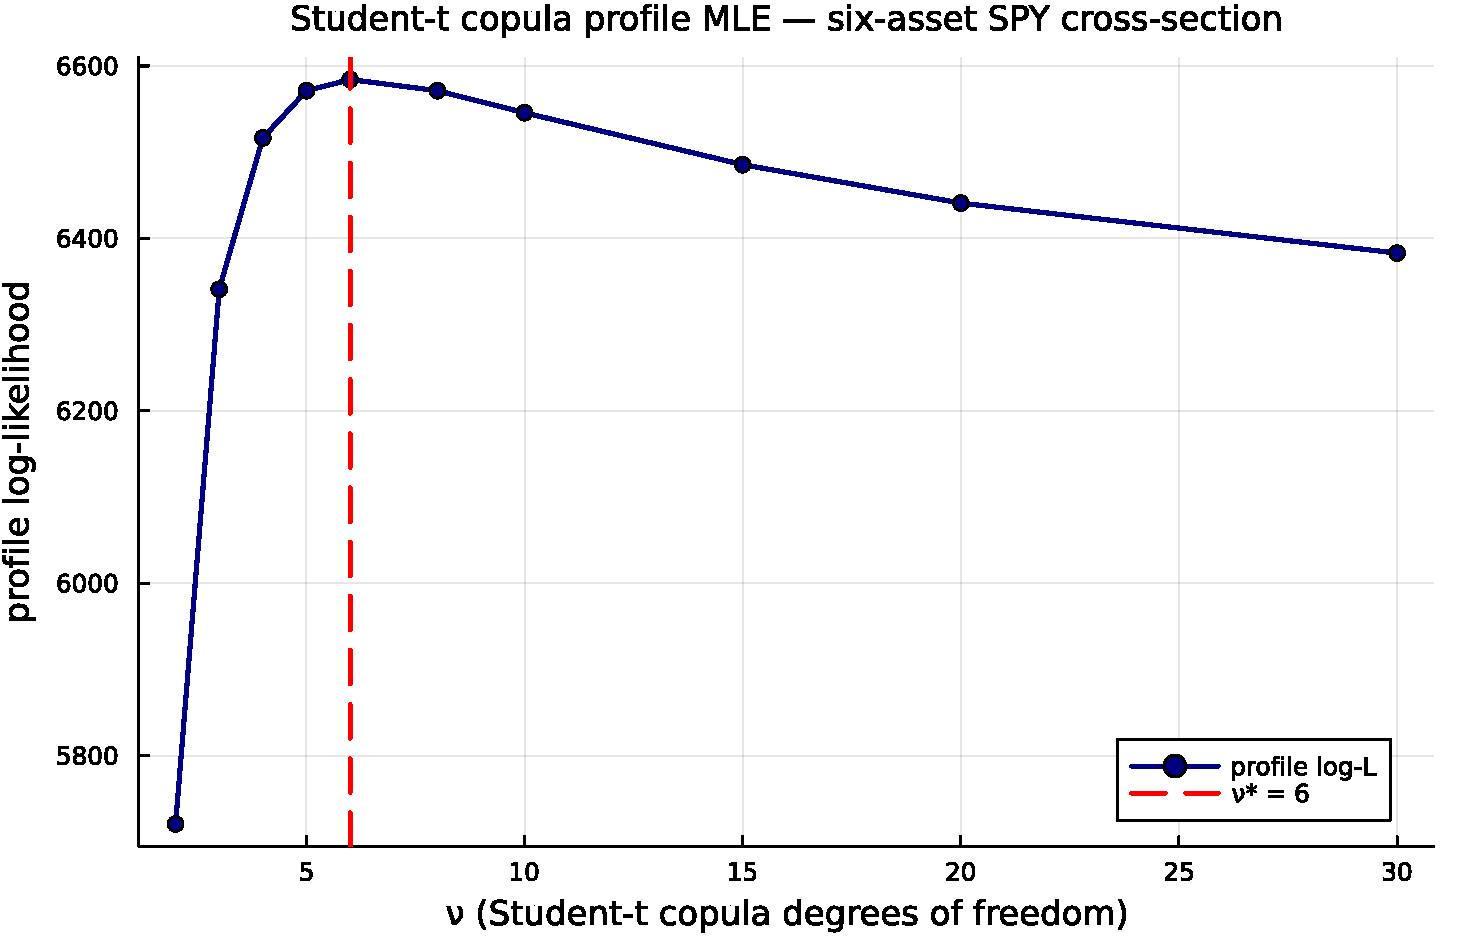
\includegraphics[width=0.70\textwidth]{sections/figs/Fig-v7-Copula-Profile.pdf}
\caption{Profile log-likelihood of the Student-t copula on the six-asset SPY cross-section. The dashed red line marks the profile MLE $\nu^{*} = 6$.}
\label{fig:copula_profile}
\end{figure}

\subsection{Block-Bootstrap Baseline}
\label{sec:block_bootstrap_supp}

Table~\ref{tab:block_bootstrap} reports the full seven-metric panel for the stationary block bootstrap at block length $b = 10$ trading days, the temporally-aware non-parametric baseline added to Table~\ref{tab:model_comparison}.

\begin{table}[h]
\centering
\small
\caption{Stationary block bootstrap (block length $b = 10$ trading days) on SPY (1000 paths, seed = 20260420).}
\label{tab:block_bootstrap}
\begin{tabular}{l cc cc c c c c}
\toprule
Window & KS & AD & Kurt & ACF-MAE & $W_1$ & $H$ & Cov \\
\midrule
IS  & 99.1 & 97.6 & 7.14 & 0.0555 & 0.084 & 0.0504 & 100.0 \\
OoS & 97.7 & 94.6 & 4.03 & 0.0547 & 0.327 & 0.2394 & 100.0 \\
\bottomrule
\end{tabular}
\end{table}

\subsection{Discrete HMM with Bin-Conditional Student-t Emissions}
\label{sec:bin_t_supp}

Table~\ref{tab:bin_t} reports the full seven-metric panel for the Bin-T NJ variant referenced in Section~\ref{sec:model_comparison}: the discrete NJ transition matrix with $K_{\text{disc}} = 13$ quantile bins, but with each bin emitting from a bin-conditional Student-t density rather than from the bin centroid.

\begin{table}[h]
\centering
\small
\caption{Discrete HMM with bin-conditional Student-t emissions on SPY (no jumps, $K_{\text{disc}} = 13$, 1000 paths, seed = 20260420).}
\label{tab:bin_t}
\begin{tabular}{l cc cc c c c c}
\toprule
Window & KS & AD & Kurt & ACF-MAE & $W_1$ & $H$ & Cov \\
\midrule
IS  & 95.5 & 90.3 & 27.28 & 0.0608 & 0.113 & 0.0919 & 84.8 \\
OoS & 97.4 & 96.7 & 5.77  & 0.0587 & 0.298 & 0.2357 & 99.0 \\
\bottomrule
\end{tabular}
\end{table}

The bin-conditional Student-t fit picks $\nu \approx 2.71$ for the two extreme bins (bins $1$ and $13$, corresponding to the lower and upper quantile tails of the IS distribution) and $\nu = 50$ (upper bracket) for the eleven central bins, which explains both the large in-sample simulated kurtosis ($27.28$) and the very thin-scale central bins ($\sigma$ $\sim$ $0.06$--$0.25$).



\subsection{GRU Deep-Generative Baseline}
\label{sec:gru_supp}

Architecture and training details for the GRU baseline used in
Section~\ref{sec:model_comparison} are summarised here.

\begin{itemize}
    \item \textbf{Architecture.} A single-layer Gated Recurrent Unit (GRU)
    with hidden dimension $H = 32$ followed by a Dense head with two
    outputs $(\mu_t, \log \sigma_t)$. Input is a single feature (the
    standardised return) over a context window of $w = 20$ trading days.

    \item \textbf{Loss.} Per-window negative log-likelihood of a Gaussian
    next-step density, equation~\eqref{eq:gru_nll}.

    \item \textbf{Optimiser.} Adam, learning rate $1.0 \times 10^{-3}$.

    \item \textbf{Training schedule.} $20$ epochs, full pass per epoch
    over $T_{\text{IS}} - w$ training windows, randomly shuffled at each
    epoch.

    \item \textbf{Numerical stability.} $\log \sigma_t$ is clamped to
    $[-6, 4]$ inside the loss to prevent gradient explosion when the
    network attempts to assign vanishingly-small variance to extreme
    observations.

    \item \textbf{Pre-processing.} The input return series is standardised
    by its in-sample mean and standard deviation; predictions are
    re-scaled back at sampling time.

    \item \textbf{Synthesis.} The trailing $w$ in-sample returns seed the
    recurrence; for each generation step the predicted Gaussian is
    sampled, the sample is appended to the context window, and the
    procedure rolls forward. The first $64$ steps are discarded as
    burn-in.

    \item \textbf{Implementation.} Julia using \texttt{Flux.jl}
    \cite{innes2018flux} with the \texttt{Optimisers.Adam} state.
    Random seed for weight initialisation, training shuffling, and per-path
    sampling: $V7\_SEED = 20260420$ with deterministic per-path sub-seeds.
\end{itemize}

The trained model is callable through the same
\texttt{simulate\_gru(model, n\_steps; seed\_window)} interface as the
CHMM and discrete-HMM models, so the seven-metric panel evaluates the GRU
on byte-identical windows to the other generators.

\begin{table}[h]
\centering
\small
\caption{GRU deep-generative baseline on SPY (single-layer, hidden $H=32$, window $w=20$, $20$ epochs, Adam $\eta=10^{-3}$, $1{,}000$ paths, seed = 20260420). Final training NLL: $0.2101$.}
\label{tab:gru}
\begin{tabular}{l cc c c c c c}
\toprule
Window & KS & AD & Kurt & ACF-MAE & $W_1$ & $H$ & Cov \\
\midrule
IS  & 2.1  & 2.7  & 2.79 & 0.0526 & 0.174 & 0.0906 & 51.5 \\
OoS & 84.2 & 85.1 & 1.72 & 0.0538 & 0.372 & 0.2441 & 78.8 \\
\bottomrule
\end{tabular}
\end{table}


\end{document}
